\usepackage{natbib}
\usepackage{graphicx,color}
\usepackage{amsmath, amssymb}
\usepackage{listings}
\usepackage{algorithm2e}
%\usepackage{paralist}
\usepackage{hyperref}
\usepackage{tcolorbox}
\usepackage{diagbox}
\usepackage{algorithm2e}
\usepackage{tikz}
\usepackage{listings}

\renewcommand{\lstlistingname}{Algorithm}
\newcommand{\bdw}{\mathbf{\Delta w}}
\newcommand{\bSig}{\pmb{\Sigma}}
\newcommand{\bmu}{\pmb{\mu}}
\newcommand{\rT}{\mathrm{T}}
\newcommand{\bb}{\mathbf{b}}
\renewcommand{\bf}{\mathbf{f}}
\newcommand{\bm}{\mathbf{m}}
\newcommand{\bp}{\mathbf{p}}
\newcommand{\br}{\mathbf{r}}
\newcommand{\bs}{\mathbf{s}}
\newcommand{\bt}{\mathbf{t}}
\newcommand{\bx}{\mathbf{x}}
\newcommand{\by}{\mathbf{y}}
\newcommand{\bw}{\mathbf{w}}

\newcommand{\bbR}{\mathbb{R}}
\newcommand{\bbE}{\mathbb{E}}
\newcommand{\cL}{\mathcal{L}}
\newcommand{\cN}{\mathcal{N}}
\newcommand{\cD}{\mathcal{D}}
\newcommand{\cT}{\mathcal{T}}
\newcommand{\cE}{\mathcal{E}}
\newcommand{\cM}{\mathcal{M}}
\newcommand{\cV}{\mathcal{V}}
\newcommand{\cC}{\mathcal{C}}
\newcommand{\bA}{\mathbf{A}}
\newcommand{\bF}{\mathbf{F}}
\newcommand{\bI}{\mathbf{I}}
\newcommand{\bJ}{\mathbf{J}}
\newcommand{\bR}{\mathbf{R}}
\newcommand{\bS}{\mathbf{S}}
\newcommand{\bT}{\mathbf{T}}
\newcommand{\bX}{\mathbf{X}}
\newcommand{\lse}{\cL_\mathrm{LSE}}
\newcommand{\bPhi}{\mathbf{\Phi}}
\newcommand{\rd}{\mathrm{d}}
\newcommand{\inv}[1]{#1^{-1}}
\newcommand{\abs}[1]{\left\lvert #1\right\rvert}
\newcommand{\norm}[1]{\left\lvert\left\lvert #1\right\rvert\right\rvert}
\newcommand{\qmark}[1]{\mbox{}\hfill\textbf{[#1]}}
\newcommand{\argmin}{\operatorname*{arg\,min}}
\newcommand{\argmax}{\operatorname*{arg\,max}}
\newcommand{\var}{\operatorname*{var}}
\newcommand{\diag}{\operatorname*{diag}}
\newcommand{\tr}{\operatorname*{Tr}}
\newcommand{\dcos}{d_\mathrm{cos}}
\newcommand{\deuc}{d_\mathrm{euc}}
\newcommand{\figref}[1]{Figure~\ref{#1}}

%\newcommand{\figref}[1]{Figure \ref{#1}}
%\renewcommand{\eqref}[1]{Equation \eqref{#1}}
\tikzset{
  treenode/.style = {shape=rectangle, rounded corners,
                     draw, align=center,
                     top color=white, bottom color=blue!20},
  root/.style     = {treenode, font=\Large, bottom color=red!30},
  env/.style      = {treenode, font=\ttfamily\normalsize},
  dummy/.style    = {circle,draw}
}

\usepackage{graphicx,color}
\usepackage{amsmath, amssymb}
\usepackage{url}
\usepackage{enumitem}
\usepackage{algorithmic}
\usepackage{algorithm}
\usepackage{listings}
\usepackage{color} 

\definecolor{mygreen}{rgb}{0,0.6,0}
\definecolor{mygray}{rgb}{0.5,0.5,0.5}
\definecolor{mymauve}{rgb}{0.58,0,0.82}
\definecolor{back}{rgb}{0.95,0.95,0.95}
\lstset{ %
  language=python, 
  backgroundcolor=\color{back},   % choose the background color
  basicstyle=\footnotesize,        % size of fonts used for the code
  breaklines=true,                 % automatic line breaking only at whitespace
  captionpos=b,                    % sets the caption-position to bottom
  numbers=left,
  numberstyle=\tiny,
  showstringspaces=false,
  xleftmargin=17pt,
  commentstyle=\color{mygreen},    % comment style
  escapeinside={\%*}{*)},          % if you want to add LaTeX within your code
  keywordstyle=\color{blue},       % keyword style
  stringstyle=\color{mymauve},     % string literal style
}
\renewcommand{\lstlistingname}{Algorithm}
\setcounter{secnumdepth}{3}

\title{Deep Learning  in Computer Vision}
\author{Amanda Cristina Fraga De Albuquerque\\
        Brendon Erick Euzebio Rus Peres\\
        Erikson Freitas de Morais\\
        Gilson Junior Soares\\
        Jose Lohame Capinga\\
        Marcella Scoczynski Ribeiro Martins}
\authorrunning{Deep Learning  in Computer Vision}

\begin{document}
\maketitle

%%Removed by Marcella since we already hava a chapter involving MLP
\section{Artificial Neural Networks} \label{neuralnetsection}

Part of the theoretical basis underlying Deep Learning  initially emerged as models for understanding learning, that is, how the brain works. Thus, these theories became known as Neural Networks, one of the areas of Deep Learning  that has grown the most in recent years \cite{goodfellow2016}. Currently, the concepts of Neural Networks address more generic principles, not restricted to the perspective of neuroscience. Even though Neural Networks cannot explain much about the brain and cannot be suggested as realistic models of biological function, many aspects of learning still remain inspirational.

Networks were designed to acquire knowledge through a learning process. Similar to what happens in the brain, interactions between neurons, or synaptic weights, are responsible for storing knowledge. In practical terms, knowledge of a network would be the ability of a machine to autonomously perform complex functions, such as classifications and pattern recognition. Networks are also able to generalize learned information, extracting essential features from examples and guaranteeing coherent responses to new cases \cite{haykin1999}.

Even though the term Neural Network has only started to gain prominence in recent years, the first theoretical studies began around 1940 \cite{goodfellow2016}. One of the first published works was ``A Logical Calculus of the Ideas Immanent in Nervous Activity'' of 1943 \cite{mcculloch1943}, in which the authors, Warren McCulloch and Walter Pitts, presented an artificial model of a neuron from the theory of logical networks of nodes \cite{goodfellow2016}.

Figure \ref{fig:figure103} presents a simplification of a biological neuron, divided into three main parts: the cell body, dendrites, and axon. A neuron receives information, or nerve impulses, from the dendrites. This information is processed in the cell body and new impulses are transmitted through the axon to other neurons. The communication between neurons, the synapse, controls the transmission of impulses, determining the flow of information based on the strength of the received signal \cite{haykin1999}.

\begin{figure}
    \centering
    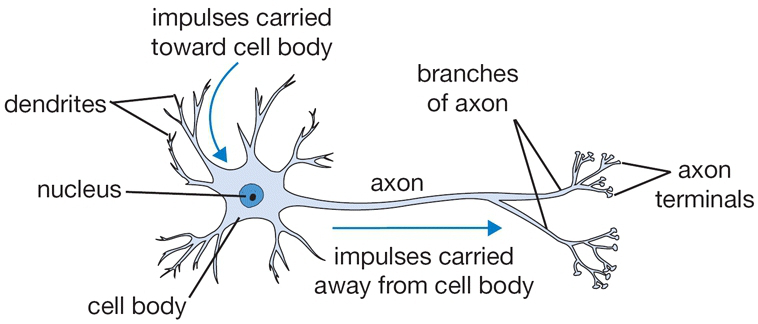
\includegraphics[scale=0.4]{"Part 3 - Learning Systems/Supervised Learning/Deep Learning/images/figure103.png"}
    \caption{Representation of a biological neuron \cite{img:neuronCS}.}
    \label{fig:figure103}
\end{figure}

By analogy to the previous paragraph, McCulloch and Pitts mathematically described an artificial neuron as a model with multiple input terminals $x_m$, representing the dendrites, and only one output point $y_k$, such as an axon Figure \ref{fig:figure104}. To simulate the behavior of synapses, each input $x_m$ is associated with a weight $w_{km}$, and the sum represents the received signal strength $v_k$.

\begin{figure}
    \centering
    \includegraphics[scale=0.7]{"Part 3 - Learning Systems/Supervised Learning/Deep Learning/images/figure104.png"}
    \caption{Mathematical representation of an artificial neuron.}
    \label{fig:figure104}
\end{figure}

The response signal is established by an activation function $\varphi$ applied to the weighted sum value. This function presents threshold behavior, Equation \ref{thresholdactivation}, in which the output is 1 or 0 according to the threshold value Figure \ref{fig:figure105}. The model can also include a bias $b_k$ in the summation to increase the degree of freedom of the activation function and ensure that a neuron does not have a null output even if the received signals are null. The bias value is adjusted along with synaptic weights \cite{haykin1999}.

\begin{equation}
\label{thresholdactivation}
y_k=\varphi(\upsilon_k)=
\begin{cases}
 1 \text{ if } \upsilon_k > 0 \\ 
 0 \text{ if } \upsilon_k \leq 0 
\end{cases}  
\end{equation}

\begin{figure}
    \centering
    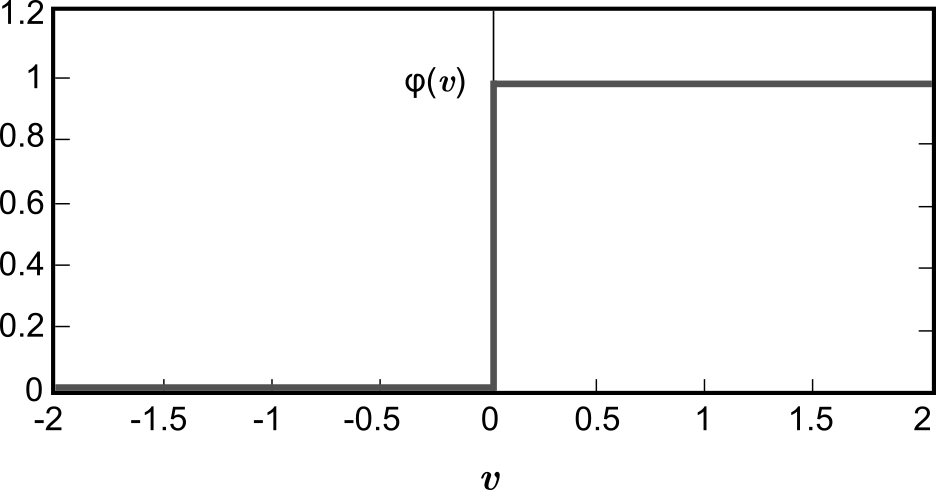
\includegraphics[scale=0.55]{"Part 3 - Learning Systems/Supervised Learning/Deep Learning/images/figure105.png"}
    \caption{Threshold Activation Function.}
    \label{fig:figure105}
\end{figure}

The model proposed by McCulloch and Walter Pitts could perform classifications in two categories. However, the weights needed to be adjusted manually as they did not have the ability to learn \cite{goodfellow2016}. One of the first discussions of learning rules in synaptic weight corrections was published in 1949 in Donald Hebb's book The Organization of Behavior \cite{haykin1999}. In Hebb's postulate, it is shown that the connection between neurons is strengthened each time it is used, thus, the neural pathways in the brain are continually modified and form clusters.

The first neural network capable of learning category weights was the Perceptron introduced by Frank Rosenblatt in 1958 \cite{haykin1999}. Perceptron had an architecture similar to Figure \ref{fig:figure106}, a single-layer network in addition to input and supervised learning. Initially, high expectations were raised about the possible applications of Perceptron, however, limitations soon began to be highlighted, many described in the book by Marvin Minsky and Seymour Papert published in 1969 \cite{minsky1969perceptrons}. One of the limitations is that the single-layer Perceptron performs only the classification of patterns that are linearly separable into two categories, which cannot, for example, represent the logic operator XOR, which is not linearly separable \cite{haykin1999}.


\begin{figure}
    \centering
    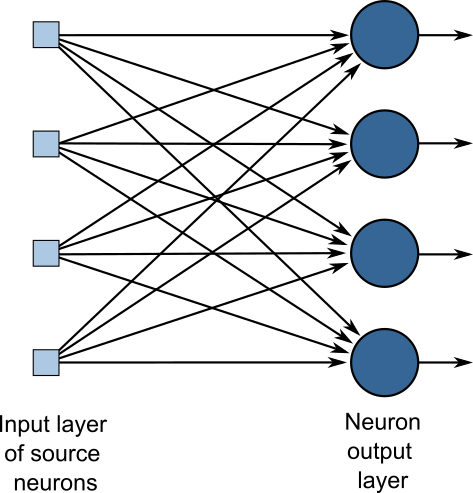
\includegraphics[scale=0.65]{"Part 3 - Learning Systems/Supervised Learning/Deep Learning/images/figure106.png"}
    \caption{One layer network architecture.}
    \label{fig:figure106}
\end{figure}

The negative image about Perceptron and its technological limitations diminished the popularity of neural networks, which reduced the number of researches in the area until the 1980s \cite{goodfellow2016}. Interest in neural networks began to increase, mainly due to the use of the distributed parallel processing approach, as applied to the backpropagation algorithm presented by Rumelhart, Hinton and Williams in 1986 \cite{rumelhart1986learning}. Backpropagation is the most widely used algorithm for Deep Learning  to date and was crucial to the training of MLP \cite{haykin1999}.

\section{MLP network}

For the multilayer Perceptron network to learn, it would be necessary to back-propagate the errors backwards between the layers, making possible the minimization of the cost function. The need to calculate the error derivative implied the appearance of activation functions different from those used in the original Perceptron model, without an abrupt activation, 0 or 1(Figure \ref{fig:figure105}) \cite{haykin1999}.  Considering that activation functions are one of the elements used to include nonlinearity, a key point for models not to be limited to linearly separable patterns, the approach was to incorporate nonlinear functions, but "well behaved" ones, that is, which are “almost” linear, continuous and derivable.

As the activation functions are responsible for the intermediation of responses between layers, nonlinear formats that do not radically alter the network response should be considered. The profiles that were closest to these behaviors are those of the sigmoid functions: the hyperbolic tangent and the logistic function \cite{rateke1999}.

The sigmoid function has an S-shape, where at the ends the function has a constant behavior, which is evident in the graph of the logistic function (Figure \ref{fig:figure107}). The parameter $a$ of the logistic equation(Equation \ref{eq:logistic}), allows to parameterize the behavior of the function, changing the slope. The higher the value of $a$, the more the sigmoid function approaches the threshold function, Figure \ref{fig:figure105}.

\begin{figure}
    \centering
    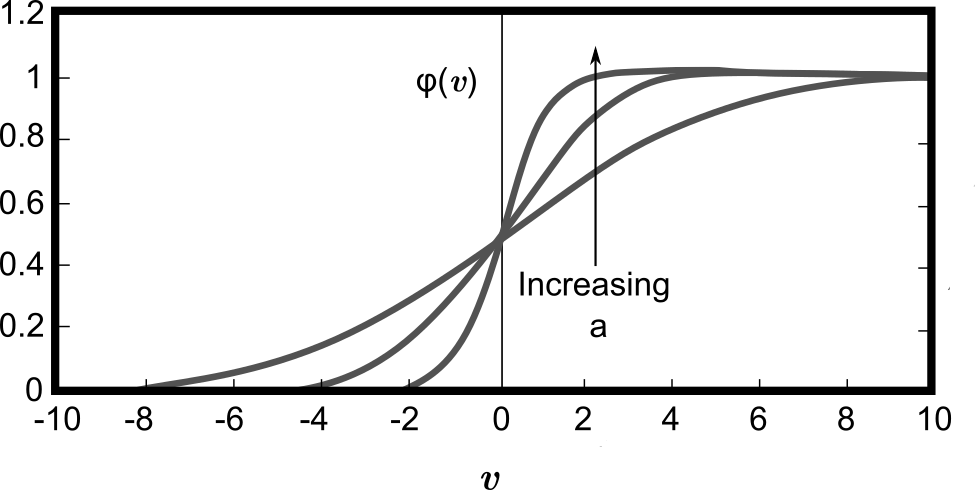
\includegraphics[scale=0.55]{"Part 3 - Learning Systems/Supervised Learning/Deep Learning/images/figure107.png"}
    \caption{Sigmoid function.}
    \label{fig:figure107}
\end{figure}

\begin{equation}
\label{eq:logistic}
\varphi(\upsilon)=
 \frac{1}{1+exp(-a)}
\end{equation}

Unlike the threshold function that takes values 0 or 1, the logistic function has results in a continuous interval between 0 and 1 \cite{haykin1999}. The sigmoid function is also differentiable, whereas the threshold function is not. An antisymmetric form of the sigmoid is the hyperbolic tangent function (Equation \ref{tanh}). The hyperbolic tangent function is defined in the interval [$-$1,1], which allows the sigmoid function to assume negative values as well \cite{haykin1999}.

\begin{equation}
\label{tanh}
\varphi(v)=tanh(av)
\end{equation}


When proposing an efficient method for training multilayer Perceptrons, it became interesting to include one or more layers of hidden neurons between the input and output layers. The combination of more layers allowed the network to be implemented for more complex problems, not restricted to the linear transformations of the original Perceptron model. Through hidden layers, it is possible to progressively extract important characteristics that define input patterns \cite{haykin1999}.

The initially proposed mathematical neuron was extended to a structure of processing elements connections, the network nodes. The elements were organized in layers, and different connection configurations were proposed. The most popular formats are defined as a neural network architecture, recognized by the number of layers in the network, number of nodes in each layer, and type of connection between nodes.

The MLP network architecture is composed of an input layer that receives the signal, an output layer that returns the result, and between them an arbitrary number of hidden layers (Figure \ref{fig:figure108}). Generally, choosing the number of nodes in the input and output layer is straightforward. For example, in an application with images, the number of neurons in the input layer could correspond to the number of pixels in the image and the output layer could be just a single neuron indicating the probability of actually being what you are looking for, the chance of a positive result. The arrangement of the intermediate layers is not so simple, however, it is often defined empirically based on the characteristics of the input data and the complexity of the problem \cite{braga1998fundamentos}.

\begin{figure}
    \centering
    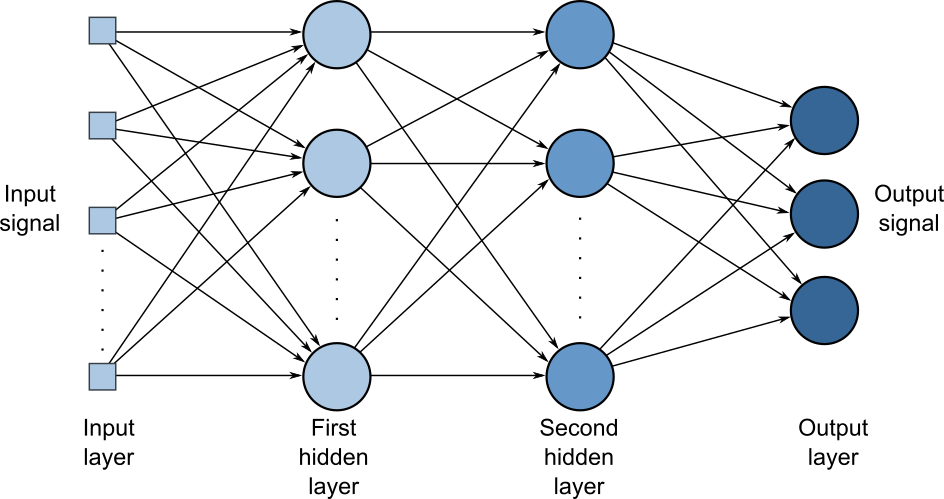
\includegraphics[scale=0.65]{"Part 3 - Learning Systems/Supervised Learning/Deep Learning/images/figure108.png"}
    \caption{MLP network architecture.}
    \label{fig:figure108}
\end{figure}

A common classification of architectures is based on the pattern of connections, two main classes being identified: direct networks (feedforward) and recurrent networks (feedback) \cite{haykin1999}. The MLP model has a feedforward type architecture, in which information propagation occurs in a single direction and nodes of the same layer are not connected to each other. The output from one layer is used as input to the next, with no loopings, that is, they are not sent back \cite{haykin1999}.
In the recurrent typologies, a feedback process occurs, in which the outputs of nodes are reinserted as inputs in previous nodes (Figure \ref{fig:figure109}). The behavior of the cycles is dynamic controlled by unit delays \cite{haykin1999}. The idea of the model is to stimulate signals in cascade effect with time dependence.

\begin{figure}
    \centering
    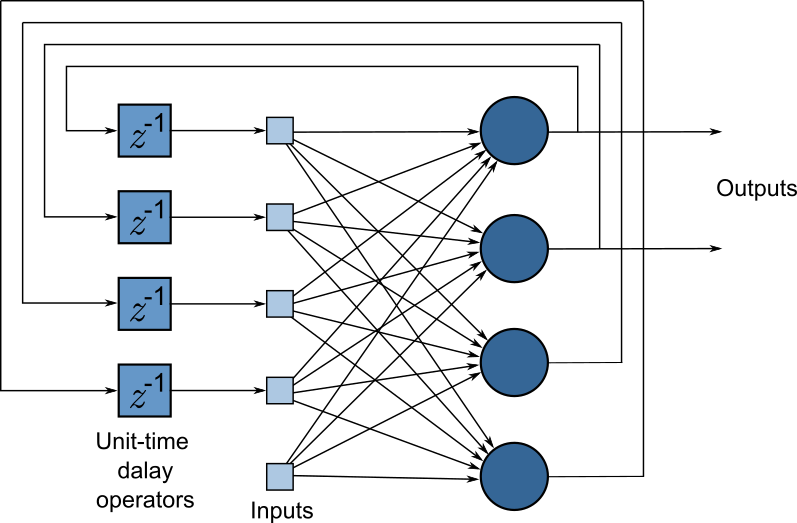
\includegraphics[scale=0.65]{"Part 3 - Learning Systems/Supervised Learning/Deep Learning/images/figure109.png"}
    \caption{recurrent network architecture \cite{haykin1999}}
    \label{fig:figure109}
\end{figure}

\section{Backpropagation}\label{backpropagation}

To explain the backpropagation algorithm in training neural networks, we will use an example of an MLP network application for number recognition. The Network Code\footnote{https://github.com/mnielsen/neural-networks-and-deep-learning} is an implementation of the online book “Neural Networks and Deep Learning” written by Michael Nielsen \cite{nielsen2015}. The training data was taken from the MNIST dataset, which contains over 60,000 scanned images of numbers written along with classification labels. The information was collected by the National Institute of Standards and Technology of the United States (NIST), and the images are in grayscale and pixel size of 28x28 as in Figure \ref{fig:figure110}.

\begin{figure}
    \centering
    
\includegraphics[scale=0.5]{"Part 3 - Learning Systems/Supervised Learning/Deep Learning/images/figure110.png"}
    \caption{An example of number zero selected from the MNIST dataset.}
    \label{fig:figure110}
\end{figure}

The original MNIST dataset is divided into two parts, one containing 60,000 images for training and the other containing 10,000 images for the testing phase, in which the accuracy of the network trained to recognize digits is evaluated. In the example of author Michael Nielsen, the original training data were also reorganized into two groups, the first with 50,000 images that were used in the training and the other part, 10,000 images, which was reserved for the validation in which the hyperparameters of the network.

Considering 28x28 pixel images, the input data was defined as vector $x$ of dimension 784, where each position corresponds to a pixel value of the image. For the output vector $y$ of the network, the dimension 10 was established, in which each position refers to a digit of 0 to 9. Thus, if an input matches the number 3 then the expected output will be the vector transposed in the form $y(x)=(0,0,0,1,0,0,0,0,0,0)^T$. Based on the format of the input and output data from the network, the example was built with a three-layer MLP network as in Figure \ref{fig:figure111}, with the first layer having 784 nodes and the last layer having 10 nodes. In the middle layer, the hidden layer, we will use 30 nodes, but it is worth noting that author Michael Nielsen defined the number of nodes after some tests, optimizing the choice of network parameters.

\begin{figure}
    \centering
    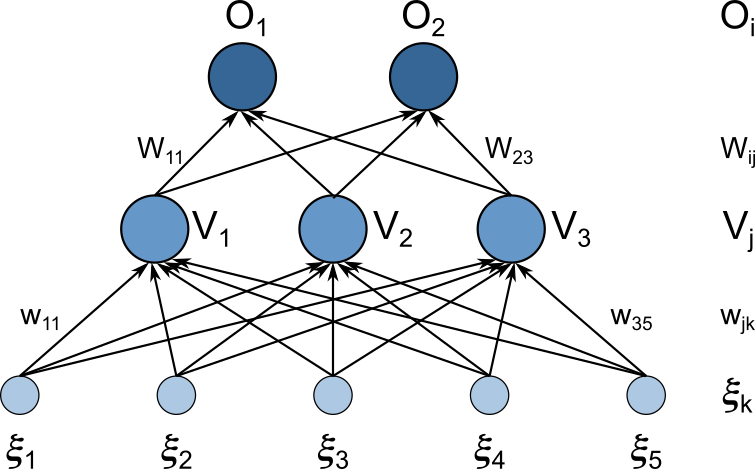
\includegraphics[scale=0.55]{"Part 3 - Learning Systems/Supervised Learning/Deep Learning/images/figure111.png"}
    \caption{MLP network with a hidden layer.}
    \label{fig:figure111}
\end{figure}

The data are taken from the zip file “mnist.pkl.gz”, subdivided into training, validation and testing, and then configured in the proposed network format.

At the Algorithm \ref{lst:classnetwork}, the network is constructed from the command “Network([784, 30, 10], cost=QuadraticCost)”, where each argument corresponds to the number of nodes in the layer. The attributes of the “Network” class include the number of layers “num\_layers,” the number of nodes in each layer “sizes,” the initial weights and bias, which are randomly generated by the “default\_weight\_initializer(),” method, and the cost function “ cost.” The cost function applied in this example is defined in the QuadraticCost class, and the quadratic error (Mean Squared Error - MSE) was used.

\begin{lstlisting}[caption={Delta method in Python},label={lst:classnetwork},language=Python]
class Network(object):
  def __init__(self, sizes, cost=QuadraticCost):
    self.num_layers = len(sizes)
    self.sizes = sizes
    self.default_weight_initializer()
    self.cost=cost
\end{lstlisting}

Next, we will present a summary of the mathematical theory of the backpropagation method and to facilitate this process we will use the nomenclature of the elements of a neural network based on the book “Introduction To The Theory Of Neural Computation” \cite{hertz2018}. In the training of a network like the one in Figure \ref{fig:figure111}, a training set is presented as $\{\xi_k^\mu,\zeta_i^\mu\}$, in which each pattern presented $(\mu=1,2,\dots,p)$ corresponds to a pair: input $(\xi_k^\mu)$ and expected output $(\zeta_i^\mu)$. In this example, the number of patterns in training is $p=50000$. The index $k$ in the input layer references the value at each node of the layer, and the index $i$ to the nodes of the output layer. The final response from the network is labeled $O_i$ and the hidden layer output signal is $V_j$. The connection between the input layer and the hidden layer is established by the weights $w_{jk}$, and the weights $W_{ij}$ connect the output layer with the middle one.

Backpropagation is a supervised method in which training takes place in two phases \cite{haykin1999}. In the forward step, an input is presented to the network and, according to the connections established between the layers, the response signals are successively propagated to the output layer, generating a result that is expected to be the closest to the standard. Each node of a subsequent layer connects with all nodes of the previous layer, and the signal received by this node is a weighting of the weights of all connections. The input signal from each node is biased and passed to the next layer as a response to an activation function $g$. The output response of a node will be called $V_j$ if the signal goes to an intermediate layer, or $O_i$ if it is directed to the output layer.

Imagine that a node $j$ in the middle layer receives as input:

\begin{equation}
\label{xisum1}
h_j^\mu=\sum_{k}w_{jk}\xi_k^\mu
\end{equation}

And produces in response:
\begin{equation}
\label{vequal}
V_j^\mu=g(h_j^\mu)=g(\sum_kw_{jk}\xi_k^\mu)
\end{equation}

Thus, a node in the output layer receives the propagated signal as input:
\begin{equation}
\label{sumsums}
h_i^\mu=\sum_kW_{ij}V_j^\mu=\sum_kW_{ij}g(\sum_kw_{jk}\xi_k^\mu)
\end{equation}

generating as a response from the output of the network:
\begin{equation}
\label{outeq}
O_i^\mu=g(h_i^\mu)=g(\sum_kW_{ij}V_j^\mu)=g(\sum_kW_{ij}g(\sum_kw_{jk}\xi_k^\mu))
\end{equation}

At the Algorithm \ref{lst:feedforward}, the forward phase is represented by the following method:

\begin{lstlisting}[caption={Delta method in Python},label={lst:feedforward},language=Python]
feedforward(self, a):
  for b, w in zip(self.biases, self.weights):
    a = sigmoid(np.dot(w, a)+b)
  return a
\end{lstlisting}

At the Algorithm \ref{lst:sigmoid}, the activation function is the logistic function defined by the “sigmoid()” method and its derivative is calculated in the “sigmoid\_prime()” method.

\begin{lstlisting}[caption={Delta method in Python},label={lst:sigmoid},language=Python]
sigmoid(z):
  return 1.0/(1.0+np.exp(-z))
 
sigmoid_prime(z):
  return sigmoid(z)*(1-sigmoid(z))
\end{lstlisting}

In the second phase, backward, the weights and bias are corrected layer by layer, from the network's output to its input, in an iterative process so that the output $O_i$ is closer and closer to the expected pattern $\zeta_i$, reducing the error \cite{haykin1999}. One way to assess how the error is reduced in relation to parameter changes is to determine an error function, or cost, dependent on weights and bias. According to Equation \ref{mserror}, we adopt the mean squared error (MSE) as a cost function.

\begin{equation}
\label{mserror}
E[w]=\frac{1}{2}\sum_{\mu i}[\zeta_i^\mu-O_i^\mu]^2 = \frac{1}{2}[\zeta_i^\mu - g(\sum_kW_{ij}g(\sum_kw_{jk}\xi_k^\mu))]^2
\end{equation}
At the Algorithm \ref{lst:fn}, the cost function (MSE) is presented in the “fn()” method in the “QuadraticCost” class:

\begin{lstlisting}[caption={Delta method in Python},label={lst:fn},language=Python]
fn(a, y):
  return 0.5*np.linalg.norm(a-y)**2
\end{lstlisting}



Error reduction involves an optimization process, called gradient descent, which seeks to determine the parameters (weights and bias) that minimize the cost function \cite{nielsen2015}. In this method, the error variation can be written as partial derivatives of the error as a function of the weights, composing the error gradient vector. As the gradient vector points towards the greatest increase in error, the variation in weights is given by the negative gradient, ensuring a faster error reduction. Thus, according to Equation \ref{minimizeError}, the descending gradient rule applied to the connections between the hidden and output layer can be written as:

\begin{equation}
\label{minimizeError}
\Delta W_{ij}=-\eta\frac{\partial E}{\partial W_{ij}}=\eta\sum_\mu[\zeta_i^\mu-O_i^\mu]g'(h_i^\mu)V_j^\mu=\eta\sum_\mu\delta_i^\mu V
\end{equation}

\begin{equation*}
\delta_i^\mu=[\zeta_i^\mu-O_i^\mu]g'(h_i^\mu)
\end{equation*}

The weight modification formula is known as the delta rule and receives the term $\eta$, the learning rate, to promote a gradual correction, without sudden changes \cite{nielsen2015}. The term $g'$ refers to the derivative of the activation function and appears in the formula due to the derivation of the error function. The delta rule applied in the connections between the hidden and the input layer uses the chain rule because the derivatives are in relation to the weights $w_{jk}$, which are presented as a more implicit dependence on the error. The correction of weights can be represented by Equation \ref{correcaoPesos}:

\begin{equation}
\begin{split}
\Delta w_{ij}&=-\eta\frac{\partial E}{\partial w_{jk}}\\&=-\eta\sum_\mu\frac{\partial E}{\partial V_j^\mu}\frac{\partial V_j^\mu}{\partial w_{jk}}\\&=\eta\sum_{\mu i}[\zeta_i^\mu-O_i^\mu]g'(h_i^\mu)W_{ij}g'(h_j^\mu)\xi_k^\mu
\\&=\eta\sum_{\mu i}\delta_i^\mu W_{ij}g'(h_j^\mu)\xi_k^\mu=\eta\sum_\mu\delta_j^\mu\xi_k^\mu
\end{split}
\label{correcaoPesos}
\end{equation}

\begin{equation*}
\delta_j^\mu=g'(h_j^\mu)\sum_i\delta_i^\mu W_{ij}
\end{equation*}

This rule can also be extended to networks with more than one hidden layer \cite{rateke1999}. The generalized delta rule for the m-th layer of a network can be described by Equation 1.13:

\begin{equation}
\Delta w_{pq}^m=\eta\sum_\mu\delta_p^{m,\mu}V_q^{m-1,\mu}
\end{equation}

\begin{equation}
\delta_p^{m, \mu} =
  \begin{cases}
    \text{if m is the Output layer, } &[\zeta_p^\mu-O_p^\mu]g'(h_p^{m,\mu})\\
    \text{otherwise, } &g'(h_p^{m,\mu})\sum_r\delta_r^{m+1,\mu}w_{rp}^{m+1}
  \end{cases}
\end{equation}

The correction of weights takes place considering the connections between each two layers, one closer to the output ($p$) and the other more internal ($q$). The vector $V_q$ represents the activation signal received by the layer of nodes “$p$”, and when the calculation involves the input layer and the first hidden layer this vector is the input pattern ($\xi_k^\mu$). The delta factor ($\delta$) works as a memory of the responses of the outermost layers, that is, to modify the weights backwards, it is necessary that the layer connections keep memory of the layers that were changed previously. The backpropagation algorithm is used in the training step, through the "backprop()" method in Algorithm \ref{lst:backprop}:

\begin{lstlisting}[caption={Backpropagation method in Python},label={lst:backprop},language=Python]
backprop(self, x, y):
    nabla_b = [np.zeros(b.shape) for b in self.biases]
    nabla_w = [np.zeros(w.shape) for w in self.weights]
    # feedforward
    activation = x
    activations = [x] 
    zs = [] 
    for b, w in zip(self.biases, self.weights):
        z = np.dot(w, activation)+b
        zs.append(z)
        activation = sigmoid(z)
        activations.append(activation)
    # backward pass
    delta = (self.cost).delta(zs[-1], activations[-1], y)
    nabla_b[-1] = delta
    nabla_w[-1] = np.dot(delta, activations[-2].transpose())
    for l in range(2, self.num_layers):
        z = zs[-l]
        sp = sigmoid_prime(z)
        delta = np.dot(self.weights[-l+1].transpose(),delta) * sp
        nabla_b[-l] = delta
        nabla_w[-l] = np.dot(delta, activations[-l-1].transpose())
    return (nabla_b, nabla_w)
\end{lstlisting}

As highlighted earlier, the first phase of backpropagation is feedforward. In this step, an input pattern ($x$) is received and the weights and bias randomly initialized. After the sum of the weights and bias weights between two layers, this value is saved in the vector “zs[ ],” and the result of activating this value is saved in “activations[ ].” The next layer input is the activation signal saved in “actvivation.” This process takes place from the input to the output layer, saving the activation signals from the hidden layers ($V_j$) in “activations[ ]”. In the backward pass phase, the delta($\delta$) is first calculated from the output layer response saved as the last element of the “activations[ ]” vector and the expected output pattern($y$). The delta value, in this case, is calculated from the “delta()” method of the “QuadraticCost” class as the product between the difference of the network output response ($a$) and the expected value ($y$) with the derivative of last layer activation signal as seen in Algorithm \ref{lst:delta}:

\begin{lstlisting}[caption={Delta method in Python},label={lst:delta},language=Python]
delta(z, a, y):
  return (a-y) * sigmoid_prime(z)
\end{lstlisting}

After calculating the first delta, the increment of weights ($\Delta W_{ij}$) between the last layer and the hidden layer is determined as the product of the delta ($\delta_i$) by the activation vector ($V_j$) that the last layer received as input. Weight increments are saved in the vector “nabla\_w[ ].” The deltas and weights increments of the hidden layer are obtained iteratively in the repetition structure. The calculation of the delta of the $m$ layer depends on the sum of the products of the delta calculated previously, of the outermost layer, with the weight vector of the $m$ layer. The summation value is multiplied by the derivative of the activation signal in the layer m. Then, the value of the increment of weights is obtained by the product of the current delta with the activation value received by layer $m$. After performing this same process for all layers, the function returns a vector with weight increments based on a pattern ($\xi_k^\mu,\zeta_i^\mu$), which occurs for all training patterns.

To speed up the learning process, instead of updating the weights each time a pattern is presented, author Michael Nielsen\cite{nielsen2015} suggests in his example the use of the stochastic gradient descending method. The idea is to randomly group the input patterns into what he calls a "mini-batch." In the update\_mini\_batch() method, the backprop function returns the calculated weight increment for each pattern within the batch, and these are summed in nabla-w until the entire batch is presented, and then the weights and bias are adjusted. Then the other “mini-batch” are presented until the entire training set is used, ending a training season. That is, at each time, the training set is subdivided into batches, and the weights are updated only at the end of each batch presentation as shown in Algorithm \ref{lst:batch}:

\begin{lstlisting}[caption={update\_mini\_batch() method in Python},label={lst:batch},language=Python]
update_mini_batch(self, mini_batch, eta, lmbda, n):
    nabla_b = [np.zeros(b.shape) for b in self.biases]
    nabla_w = [np.zeros(w.shape) for w in self.weights]
    for x, y in mini_batch:
        delta_nabla_b, delta_nabla_w = self.backprop(x, y)
        nabla_b = [nb+dnb for nb, dnb in zip(nabla_b, 
                delta_nabla_b)]
        nabla_w = [nw+dnw for nw, dnw in zip(nabla_w, 
                delta_nabla_w)]
    self.weights = [(1-eta*(lmbda/n))*w-(eta/len(mini_batch))*nw
                for w, nw in zip(self.weights, nabla_w)]
    self.biases = [b-(eta/len(mini_batch))*nb
                for b, nb in zip(self.biases, nabla_b)]
\end{lstlisting}

The training takes place using the “SGD()” method, which stands for descent of the stochastic gradient, in which the training set, the number of epochs, the size of the “mini\_batch\_size” grouping and the learning rate are passed as parameters.

\begin{lstlisting}[caption={SGD call in Python},label={lst:sgd},language=Python]
net.SGD(training_data,30,10,0.5, evaluation_data=test_data,
        monitor_evaluation_cost=True, monitor_evaluation_accuracy=True,
        monitor_training_accuracy=True, monitor_training_cost=True)
\end{lstlisting}

It's in the “SGD()” method”(Algorithm \ref{lst:SGD}), which occurs the subdivision of training patterns into "mini\_batch." Then, the “update\_mini\_batch()” function is called for each grouping until one epoch ends, and this is repeated for all epochs.

\begin{lstlisting}[caption={SGD method in Python},label={lst:SGD},language=Python]
SGD(self, training_data, epochs, mini_batch_size, eta,
    lmbda = 0.0, evaluation_data=None, 
    monitor_evaluation_cost=False, 
    monitor_evaluation_accuracy=False,
    monitor_training_cost=False, 
    monitor_training_accuracy=False):
  for j in range(epochs):
    random.shuffle(training_data)
    mini_batches = [training_data[k:k+mini_batch_size] 
                for k in range(0, n, mini_batch_size)]
    for mini_batch in mini_batches:
        self.update_mini_batch(mini_batch, eta, lmbda,
                                len(training_data))
    print ("Epoch %s training complete" % j)
\end{lstlisting}

Within the “SGD()” method it is possible to configure to evaluate the total error and accuracy of the network after each training period, considering both the training data and the test or validation data. To select the test data, they must be passed as parameters in “evaluation\_data”. When selecting the options “monitor\_evaluation\_cost” or “monitor\_training\_cost” the method “total\_cost()” is called(Algorithm \ref{lst:cost}) which returns the sum of the evaluated errors for the entire dataset.

\begin{lstlisting}[caption={total\_cost() method in Python},label={lst:cost},language=Python]
total_cost(self, data, lmbda, convert=False):
    cost = 0.0
    for x, y in data:
        a = self.feedforward(x)
        if convert: y = vectorized_result(y)
        cost += self.cost.fn(a, y)/len(data)
    return cost
\end{lstlisting}

After each epoch, a set of weights and bias is established, and when using the “feedforward()” method, these parameters define the output response of the network ($a$) for each input pattern ($x$). By comparing the answer ($a$) with the expected value ($y$) within the MSE cost function, method “fn()” of the class “QuadraticCost,” the error for each pattern is quantified. The “accuracy()” method in Algorithm \ref{lst:accuracy}, is used inside the “SGD()” when setting “monitor\_evaluation\_accuracy= True” or “monitor\_training\_accuracy= True.” This function returns the sum of results where the net output values matched the expected value ($y$). The network signal is calculated by the “feedforward()” function, which is used for each value ($x$) of the dataset, whether training or evaluation.

\begin{lstlisting}[caption={accuracy() method in Python},label={lst:accuracy},language=Python]
accuracy(self, data, convert=False):
    results = [(np.argmax(self.feedforward(x)), y) 
                for (x, y) in data]
    return sum(int(x == y) for (x, y) in results)
\end{lstlisting}

Considering that the values of the total error and the accuracy are calculated for each epoch, the training method “SGD()” returns four vectors inside a tuple(in Algorithm \ref{lst:return}), each one with the number of positions corresponding to the total number of epochs. Thus, if the training takes place in 30 epochs, then the first list in the tuple will have 30 elements corresponding to the total cost of the evaluation data at the end of each epoch.

\begin{lstlisting}[caption={Delta method in Python},label={lst:return},language=Python]
return evaluation_cost, evaluation_accuracy,
            training_cost,training_accuracy
\end{lstlisting}

Saved results can be plotted on graphs to visually assess network performance. A very common graph to monitor network training is the training cost, mainly because learning is guided by minimizing this curve. In Figure \ref{fig:figure113}, the cost curve for a configuration that uses the total training set (50000 images) and with 30 epochs is presented. However, it is not recommended to have only this graph as a basis to establish the network's hyperparameters, such as the learning rate and the number of training epochs. For example, Figure \ref{fig:figure114} also refers to a cost function, but for another training setup, which uses only 1000 training images and 100 epochs.

\begin{figure}
    \centering
    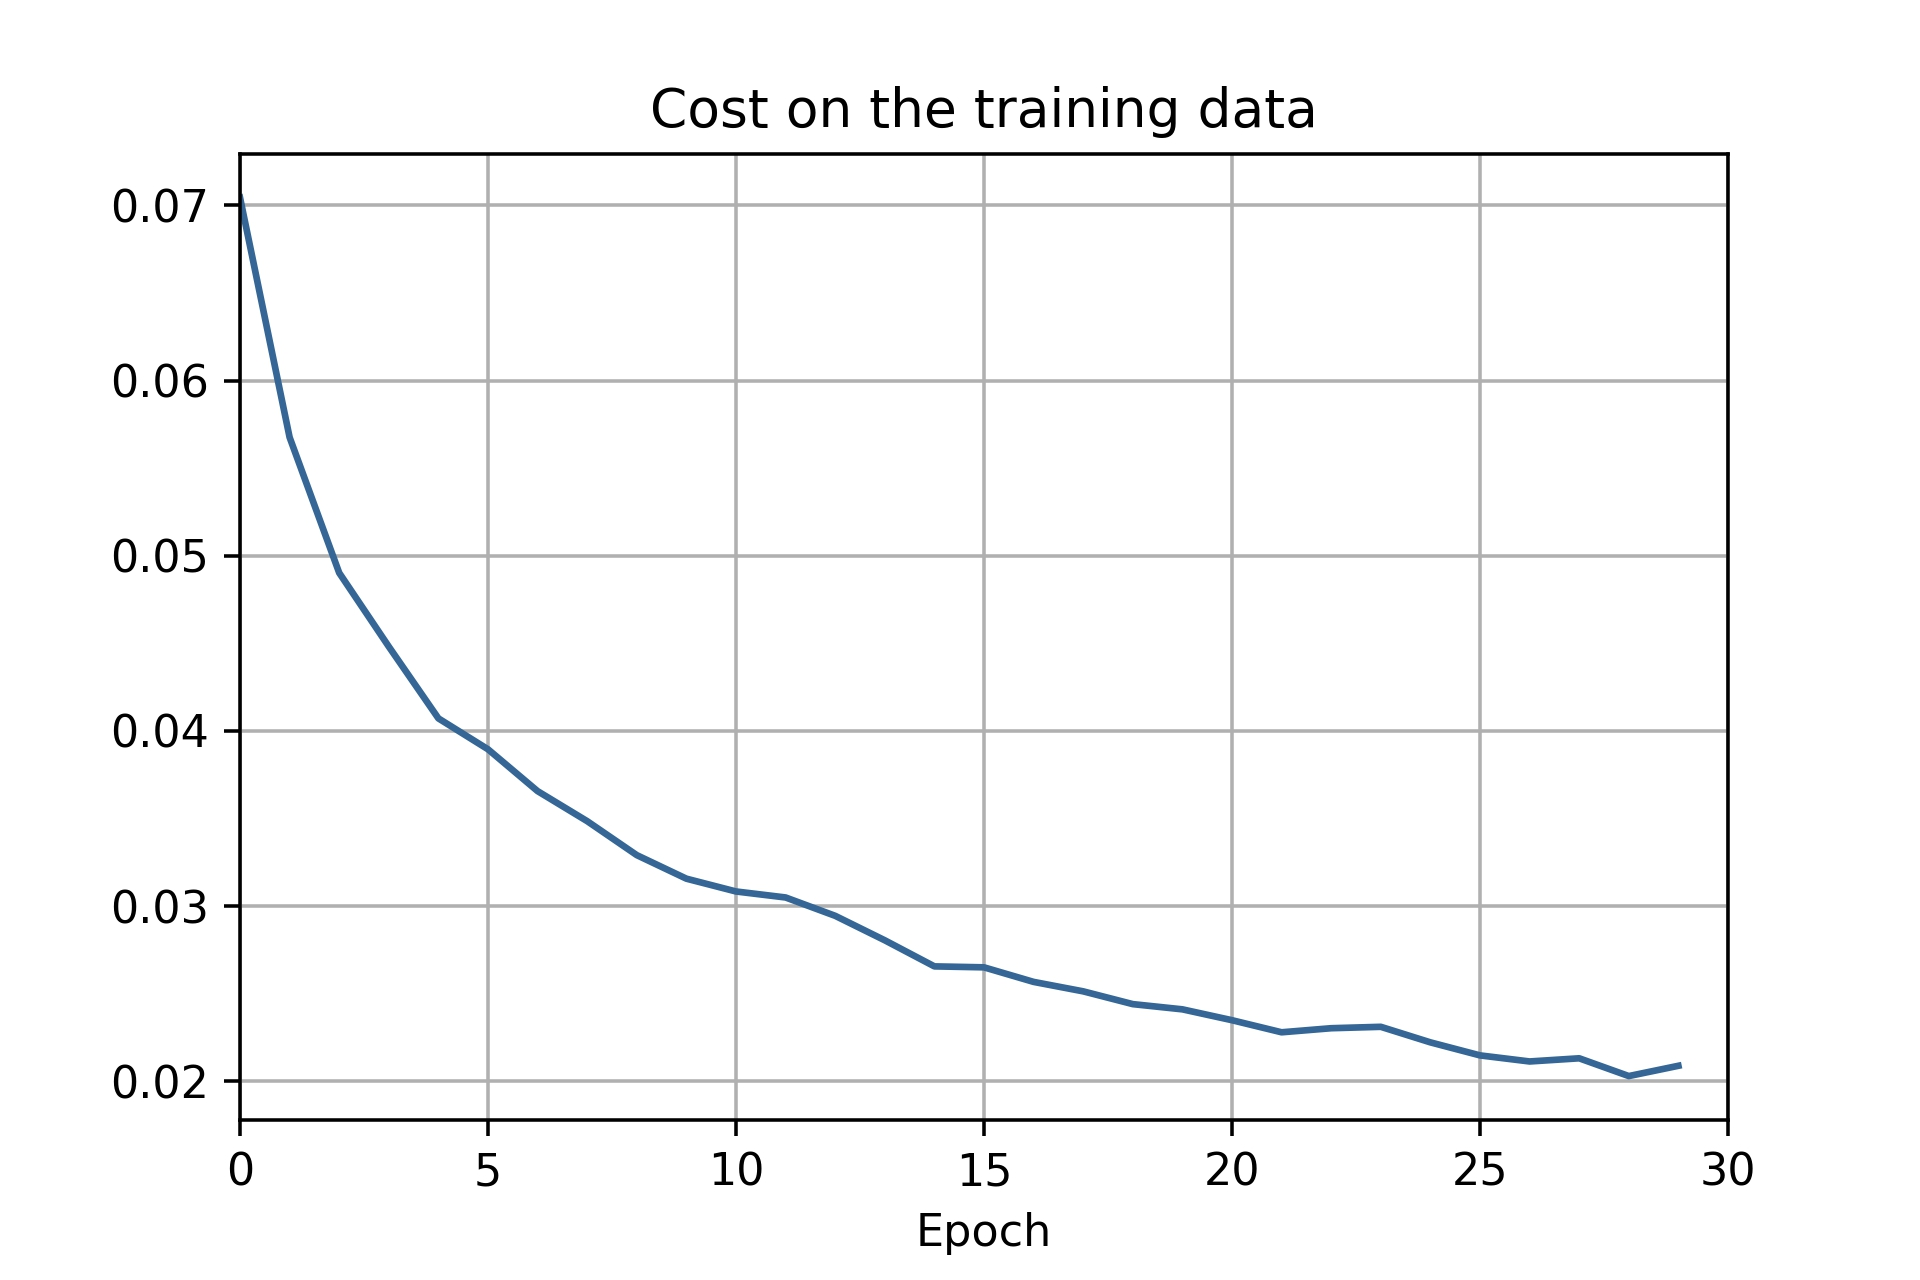
\includegraphics[scale=0.6]{"Part 3 - Learning Systems/Supervised Learning/Deep Learning/images/figure113.jpg"}
    \caption{Cost curve in training with 30 epochs and 50000 images.}
    \label{fig:figure113}
\end{figure}

\begin{figure}
    \centering
    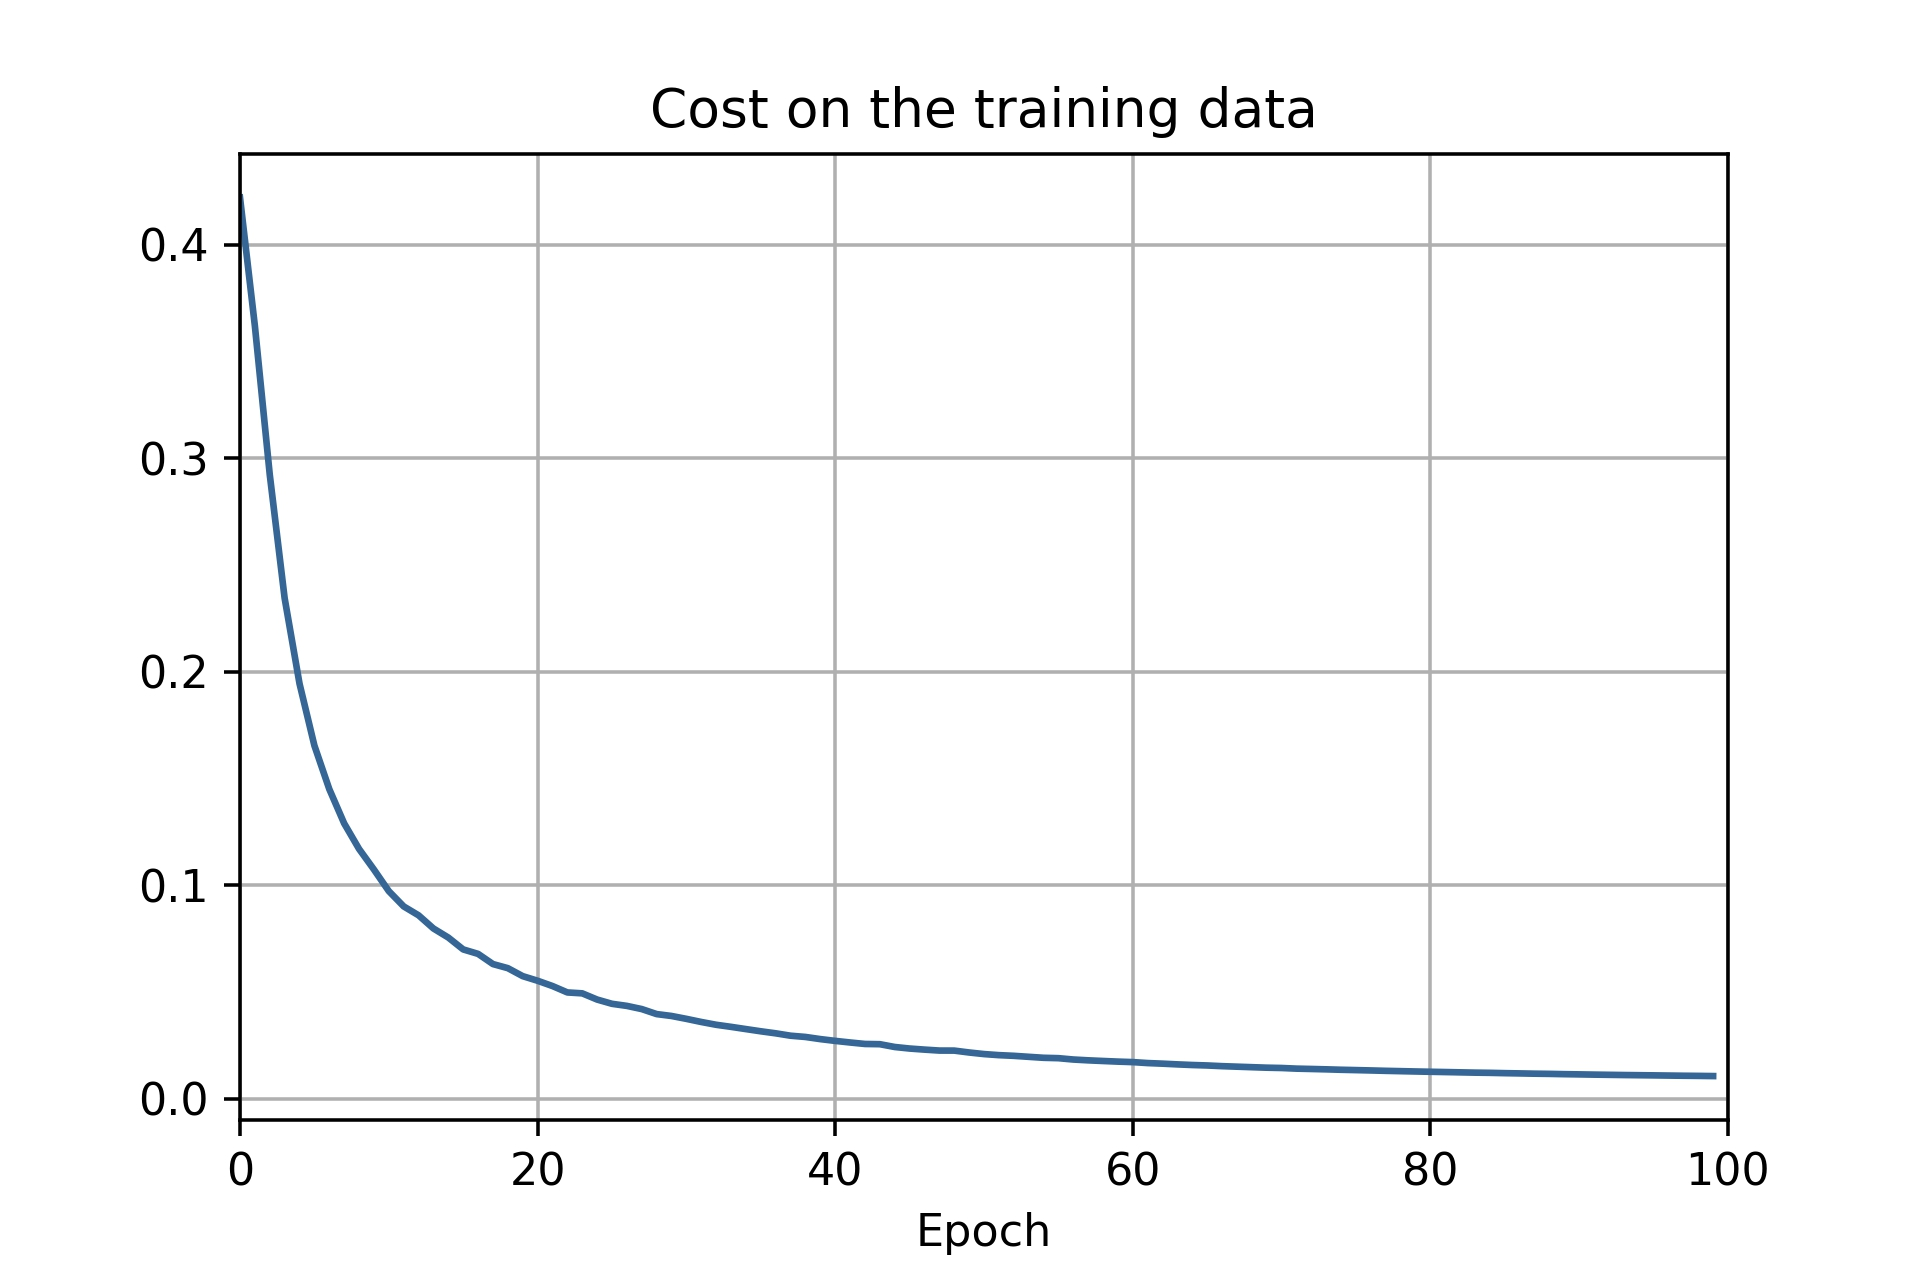
\includegraphics[scale=0.6]{"Part 3 - Learning Systems/Supervised Learning/Deep Learning/images/figure114.jpg"}
    \caption{Cost curve in training with 100 epochs and 1000 images.}
    \label{fig:figure114}
\end{figure}

At the end of the training, both networks had errors in the same order of magnitude, but the ability to recognize numbers is quite different between the two. This difference can be seen when comparing the accuracy graphs (Figures \ref{fig:figure115} and \ref{fig:figure116}) considering both training and validation data. The result of training with the entire dataset shows that the accuracy of the network for the validation data is very close to the result for the training values, a difference of 1\% . As for the situation that used only 1000 training data, the accuracy curves for the validation and training data are further apart, presenting a difference close to 14\%.

\begin{figure}
    \centering
    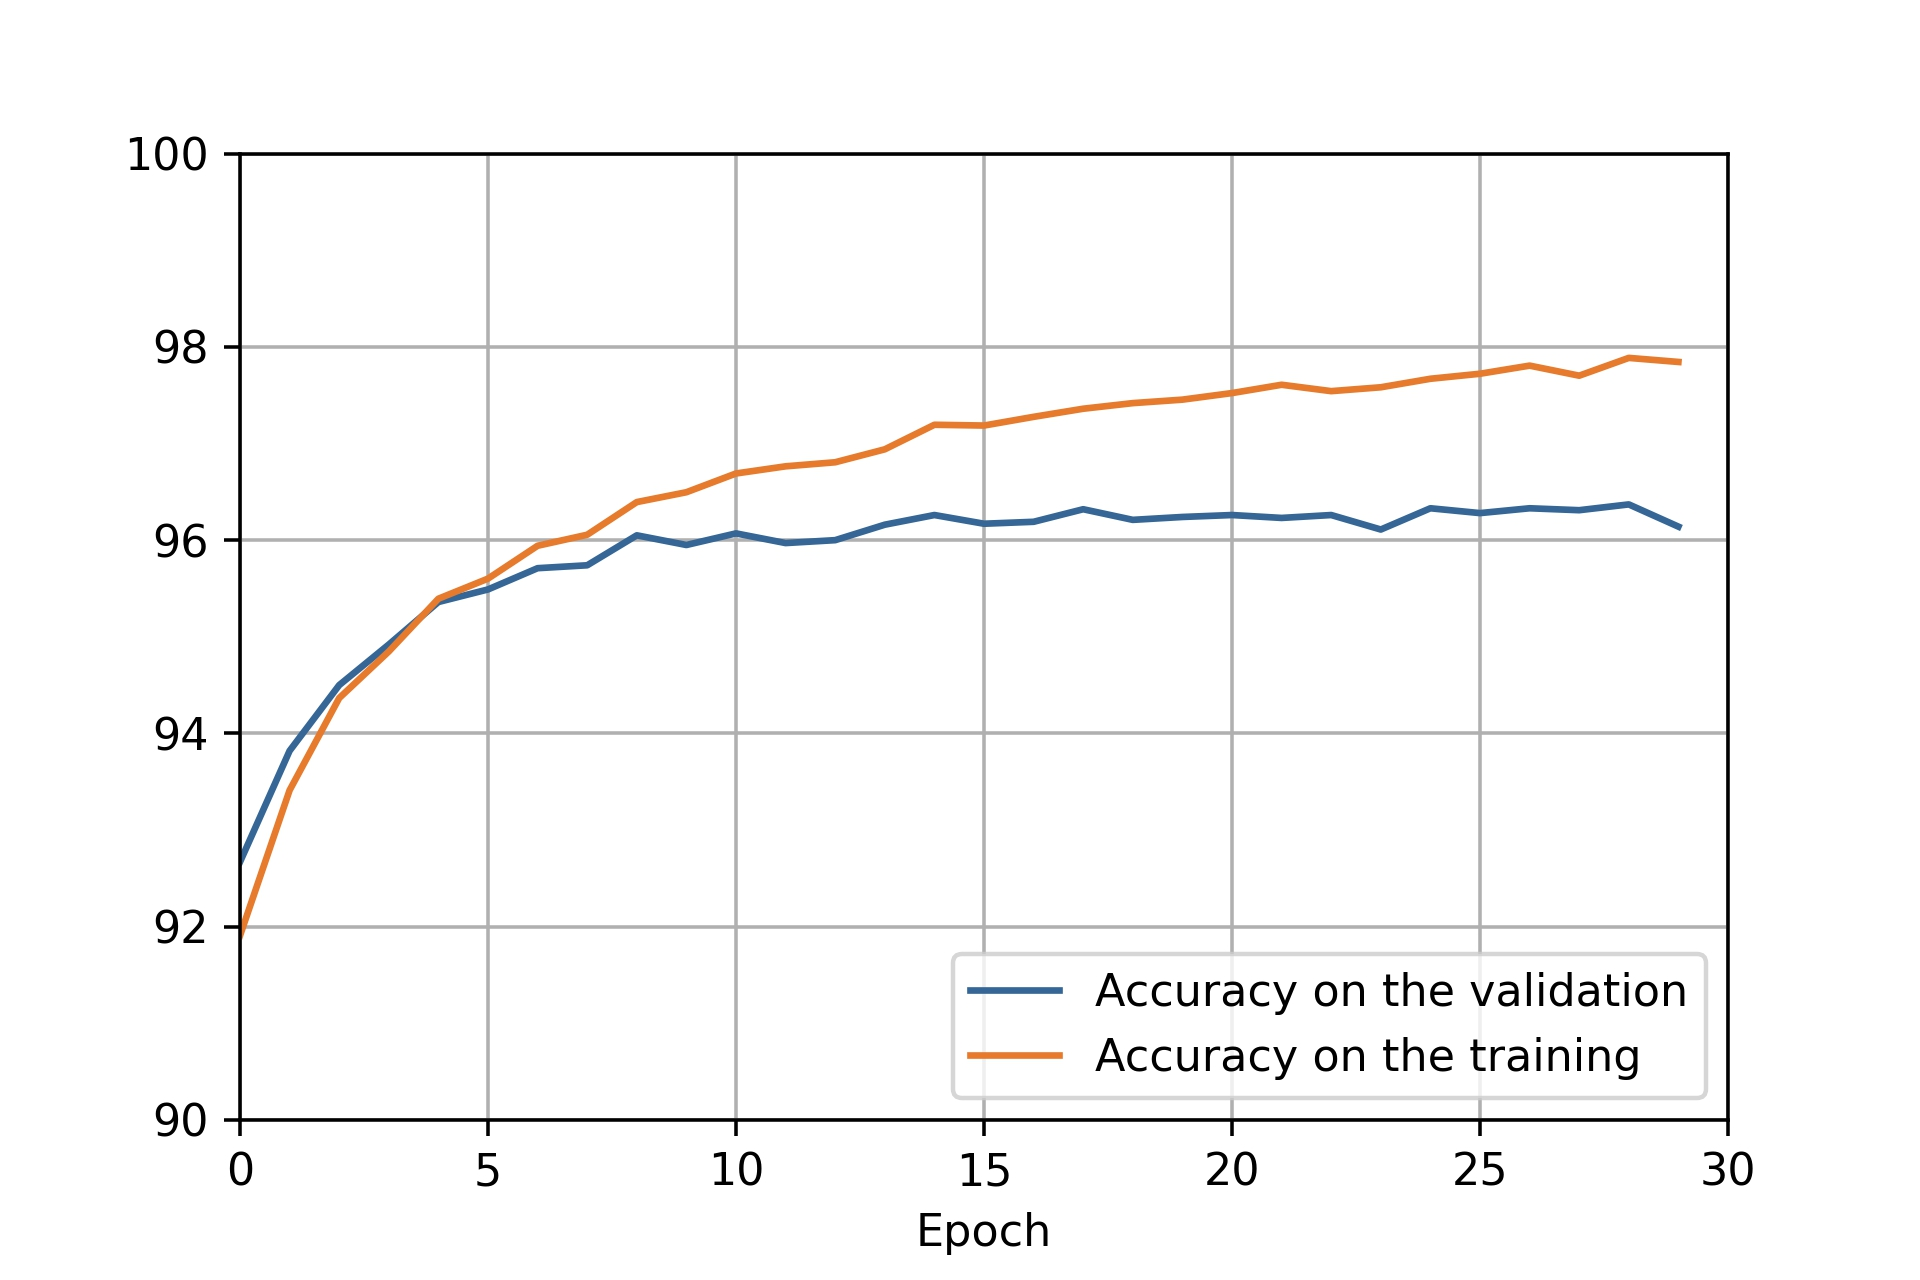
\includegraphics[scale=0.6]{"Part 3 - Learning Systems/Supervised Learning/Deep Learning/images/figure115.jpg"}
    \caption{Accuracy curves for a network trained with epochs 30 and 1000 images.}
    \label{fig:figure115}
\end{figure}

\begin{figure}
    \centering
    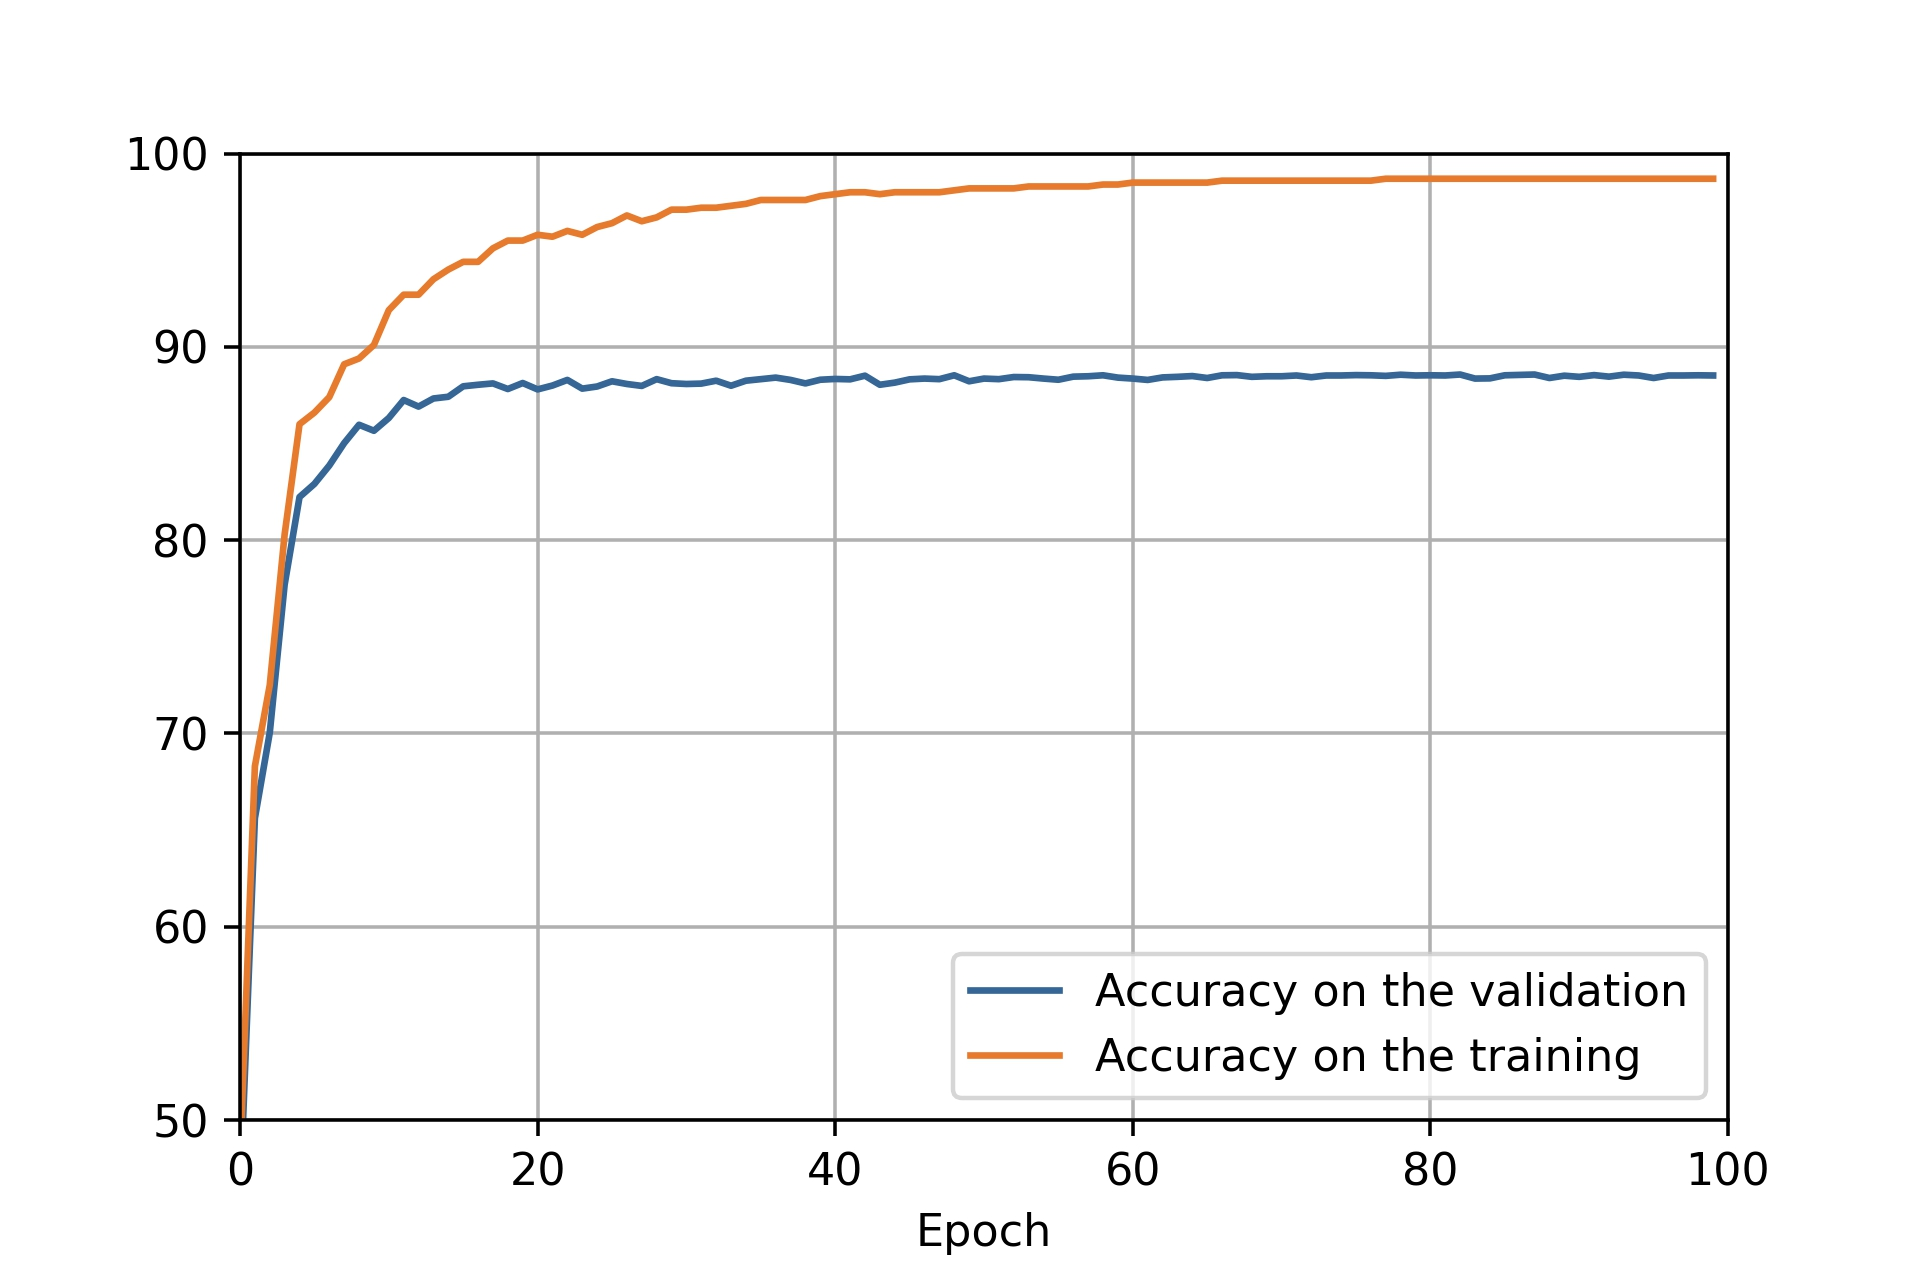
\includegraphics[scale=0.6]{"Part 3 - Learning Systems/Supervised Learning/Deep Learning/images/figure116.jpg"}
    \caption{Cost curve in training with 100 epochs and 1000 images.}
    \label{fig:figure116}
\end{figure}

By observing only the error curve, it is assumed that the network is learning until the end of the training, as the error continues to decrease. However, when analyzing the accuracy curves, it is identified that the accuracy determined by the validation data increases rapidly up to a certain time, close to 40 in the second case, and then becomes stagnant. Thus, after the 40th epoch, the network is no longer learning to generalize to the validation data, overfitting is occurring, that is, the training is not improving the network's capacity. Even though training accuracy is increasing after this time, it may be that the network is just memorizing training data, as it is no longer just sticking to the general information needed to recognize the numbers in general \cite{nielsen2015}.

The most common cases of overfitting occur when the number of training data is very low, as in this second case with only 1000 images. In this situation, the network has few examples to extract general information, often needing to increase the number of training times in order to reach a minimum performance. The greater the number of epochs, the more evident the overfiting effect may be, so it is recommended to observe when the validation accuracy starts to stagnate and get too far from the training curve \cite{nielsen2015}.

Observing the behavior of the validation accuracy is one of the methods to define how long the network should be trained, that is, the number of epochs. Validation data helps in testing different configurations of network hyperparameters such as training times, learning rate and number of nodes. Only after defining these parameters and training the network is it recommended to use the test data to really verify the accuracy of the network, using data that it has not yet had contact with \cite{nielsen2015}. A test with unknown data makes it possible to verify if the network parameters can be applied in more general cases or if they fit only in particularities of the trained data. For this reason, in most cases data is divided into three sets - training, validation and testing.
 Deep Learning is part of machine learning methods based on artificial neural networks with representation learning. %Learning can be supervised, semi-supervised or unsupervised. 
 Part of the theoretical basis underlying Deep Learning  initially emerged as models for understanding learning, that is, how the brain works. Thus, these theories are related with Deep Learning  that has grown the most in recent years \cite{goodfellow2016}.

The deep learning area has achieved excellent performance in applications, mainly due to the development of the area and the increase in computational power and the amount of available data \cite{geron2019}. 

Computer vision is another field of Artificial Intelligence (IA), as it also seeks to reproduce some of the human capabilities from autonomous systems. The main interest of computer vision is to make computers perform functions similar to human vision, being able to receive visual data and with them perform recognition, classification and analysis. It is identified that the improvement in the performance of computer vision is strongly linked with the evolution of machine learning.

The old computer vision techniques were almost entirely pipelined by hand, where the features to be extracted and the algorithms used were done manually. This made such techniques more difficult to adapt to different tasks. With the emergence of deep learning, it became possible to use these networks to perform this feature extraction work, in addition to the algorithm part, where machine learn performs the task.

\begin{figure}
    \centering
    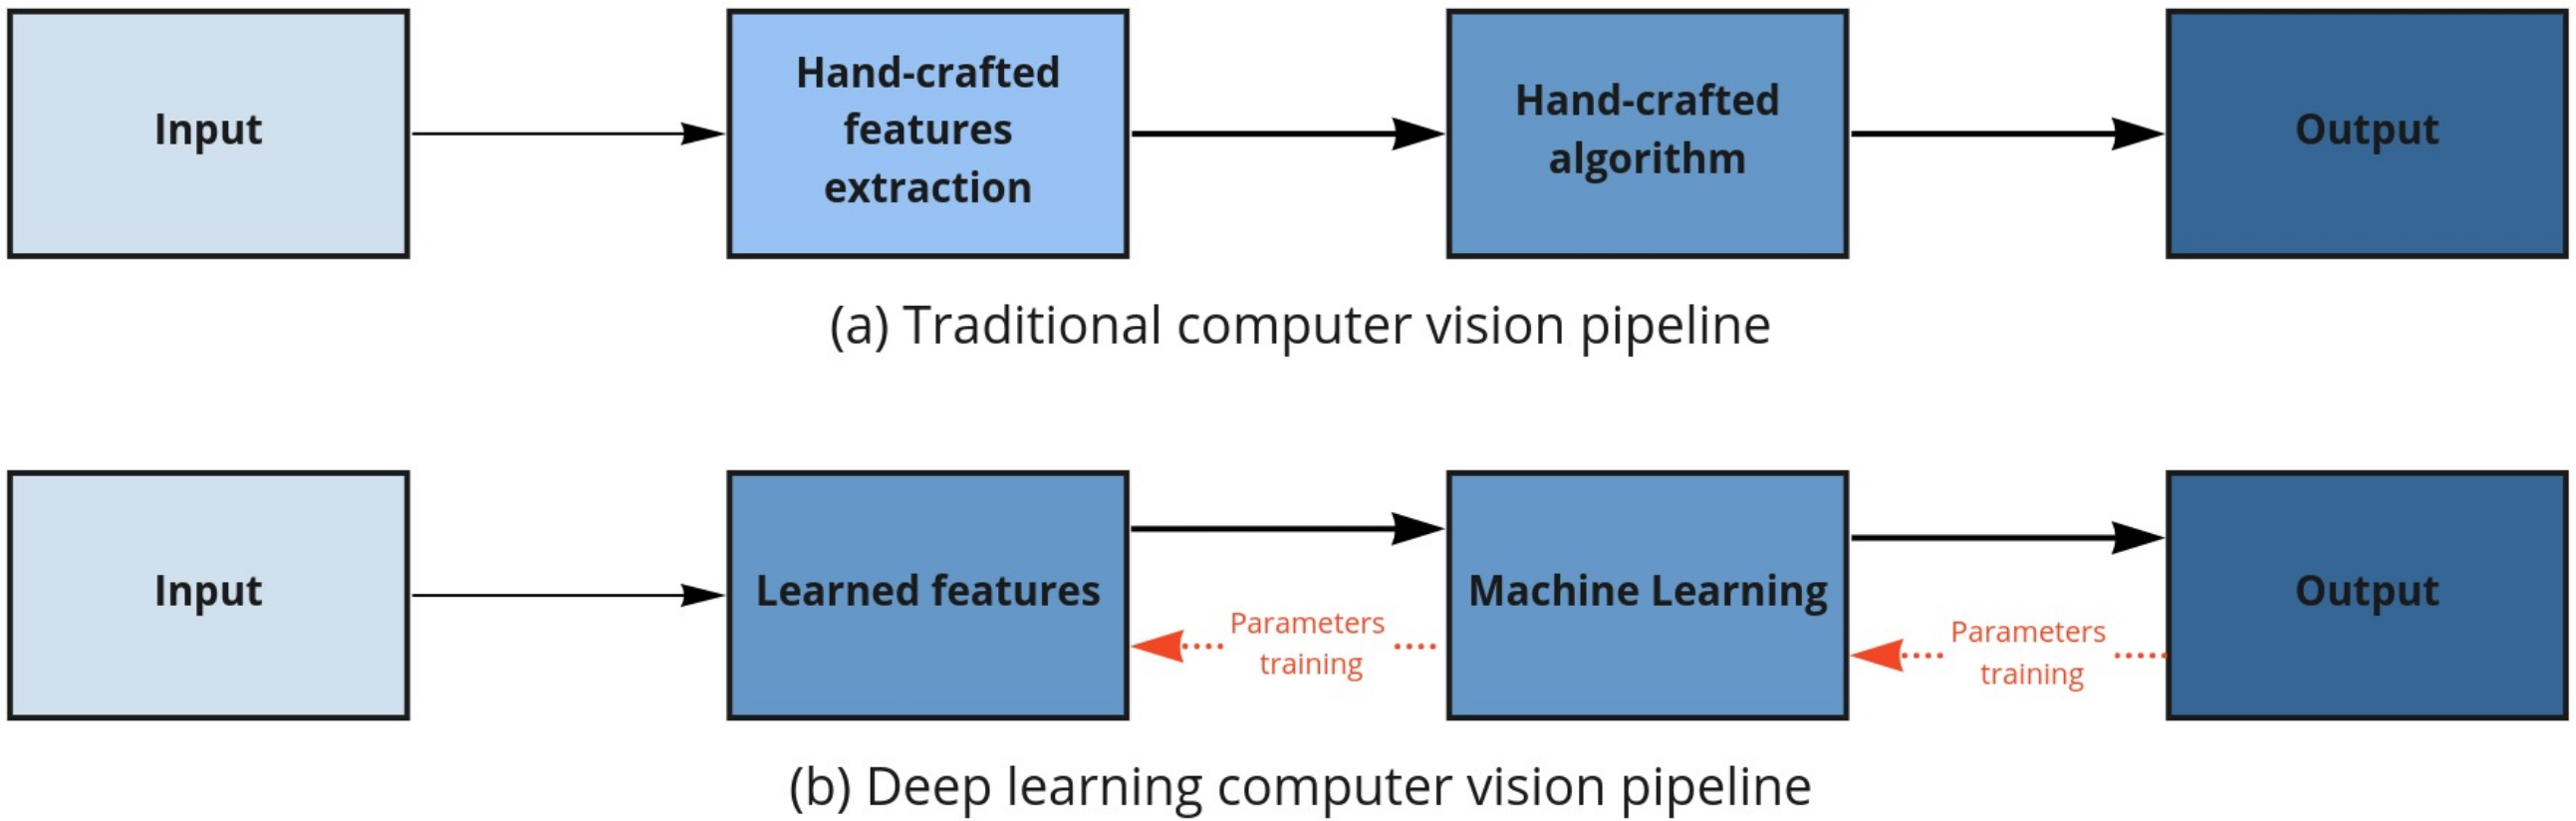
\includegraphics[scale=0.20]{images/cvpipeline.png}
    \caption{Traditional(a) and Deep learnign(b) computer vision pipelines. Inspired in \cite{szeliski2010computer}(Figure 5.2)}
    \label{fig:figurecvpipeline}
\end{figure}

In Figure \ref{fig:figurecvpipeline} we have the representation of the two types of pipeline previously mentioned. The tradicional(\ref{fig:figurecvpipeline} (a)), where the two principal steps, the selection of features to be extract and the algorithm that use these features, are hand-crafted. The Deep learning pipeline(\ref{fig:figurecvpipeline} (b)), where the model learns which features to extract and how use these features to get the desired output. The red arrow in Deep Learning pipeline shows how this type of model use information about the output to adjust the parameters of the network, and consequently, learns.

Among the many deep learning architectures, the Convolutional Neural Networks (CNN) is one of the most widely used as it is very similar to conventional NN.

\section{Convolutional Neural Networks (CNN)}

In common neural networks we basically use neurons and connections between them to build a model. Convolutional neural networks, on the other hand, have some more structures, which are the reason for their efficiency in working with images. We will see them next.


\subsection{Convolution Layers}

The operation that names the network, the convolution, is an operation performed between two functions. In our case, as we are working with images, we will use discrete convolution.
%An important point to note is that mathematically what we will call a convolution is actually a correlation, and the two are almost identical, except for the fact that in the convolution we rotate the filter (kernel) by 180\textdegree . The only advantage we gain from turning the filter before the operation is that we gain the commutative property, which is mathematically useful for proof derivation but not important in Deep Learning  implementation \cite{goodfellow2016}.

In Deep Learning  literature and libraries, including CNN's, it has become common to call the two operations convolution \cite{goodfellow2016}, so we will also use this convention, using convolution without rotating the filter, so a correlation.
The discrete correlation formula is given by:

\begin{equation}
g(x,y)=w(x,y)\star f(x,y)=\sum_{s=-a}^a\sum_{t=-b}^bw(s,t)f(x+s,y+t)
\end{equation}

Where $\star$ represents the correlation operation; $w$ is our filter (kernel), a matrix of numbers, usually with odd square size (to facilitate operations), and $f$, our image, also an matrix. And related to it we have the formula of convolution ($g$):

\begin{equation}
g(x,y)=w(x,y)\ast f(x,y)=\sum_{s=-a}^a\sum_{t=-b}^bw(s,t)f(x-s,y-t)
\end{equation}

As we can see by looking at the two equations, these operations are very simple, being basically a sum of products. In Figure \ref{fig:figure117}, we have a representation of a correlation step, where we can observe the following operation:

%corrigir orientação
\begin{equation}
\begin{split}
w*f(0,0)=\sum_{s=1}^{2}\sum_{t=1}^{2}w(s,t){f}(0-s,0-t)= \\
w(0,0)f(0,0)+w(0,1)f(0,1)+w(0,2)f(0,2) \\
+w(1,0)f(1,0)+w(1,1)f(1,1)+w(1,2)f(1,2) \\
+w(2,0)f(2,0)+w(2,1)f(2,1)+w(2,2)f(2,2)\\
=(-1)\cdot5+(-2)\cdot7+(-1)\cdot0\\
+0\cdot6+0\cdot0+0\cdot1\\
+1\cdot6+2\cdot2+1\cdot2
=-19-0+12=-7
\end{split}
\end{equation}

\begin{figure}
    \centering
    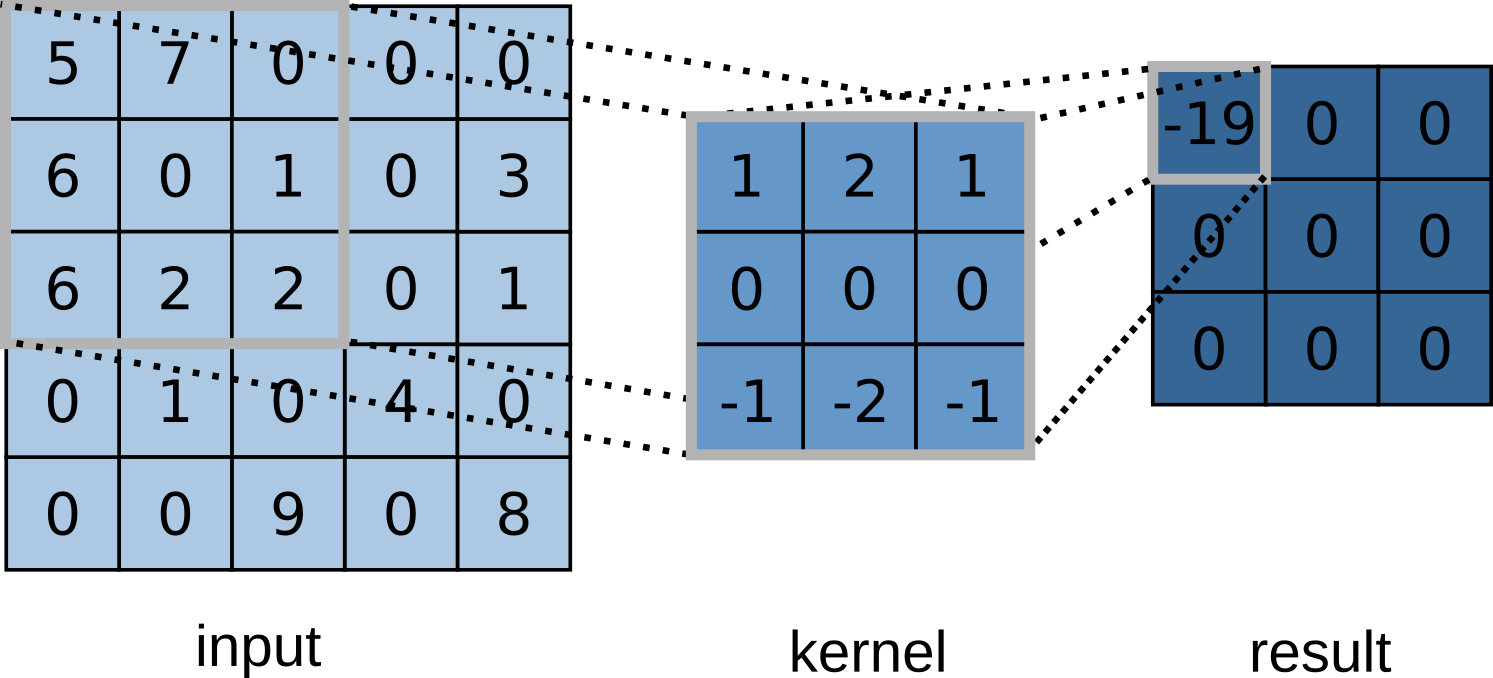
\includegraphics[scale=0.40]{images/figure117.png}
    \caption{Convolution of a 5x5 sized image with a 3x3 sized kernel and its result.}
    \label{fig:figure117}
\end{figure}

The previous example, Figure \ref{fig:figure117}, was quite simple, but we know that in many applications we won't have the input image represented by just a matrix (configuring a grayscale image) but most of the time we will be using images that contain three dimensions. In this case, we will have an image in the RGB model, where three matrices will be present, each one representing a color channel. In Figure \ref{fig:figure118}, there is an example of convolution in RGB images. We can see that now our kernel is also made up of three matrices. An important thing to note is that the number of layers in the input filter has to equal the number of channels in the image for the convolution operation to be done.

\begin{figure}
    \centering
    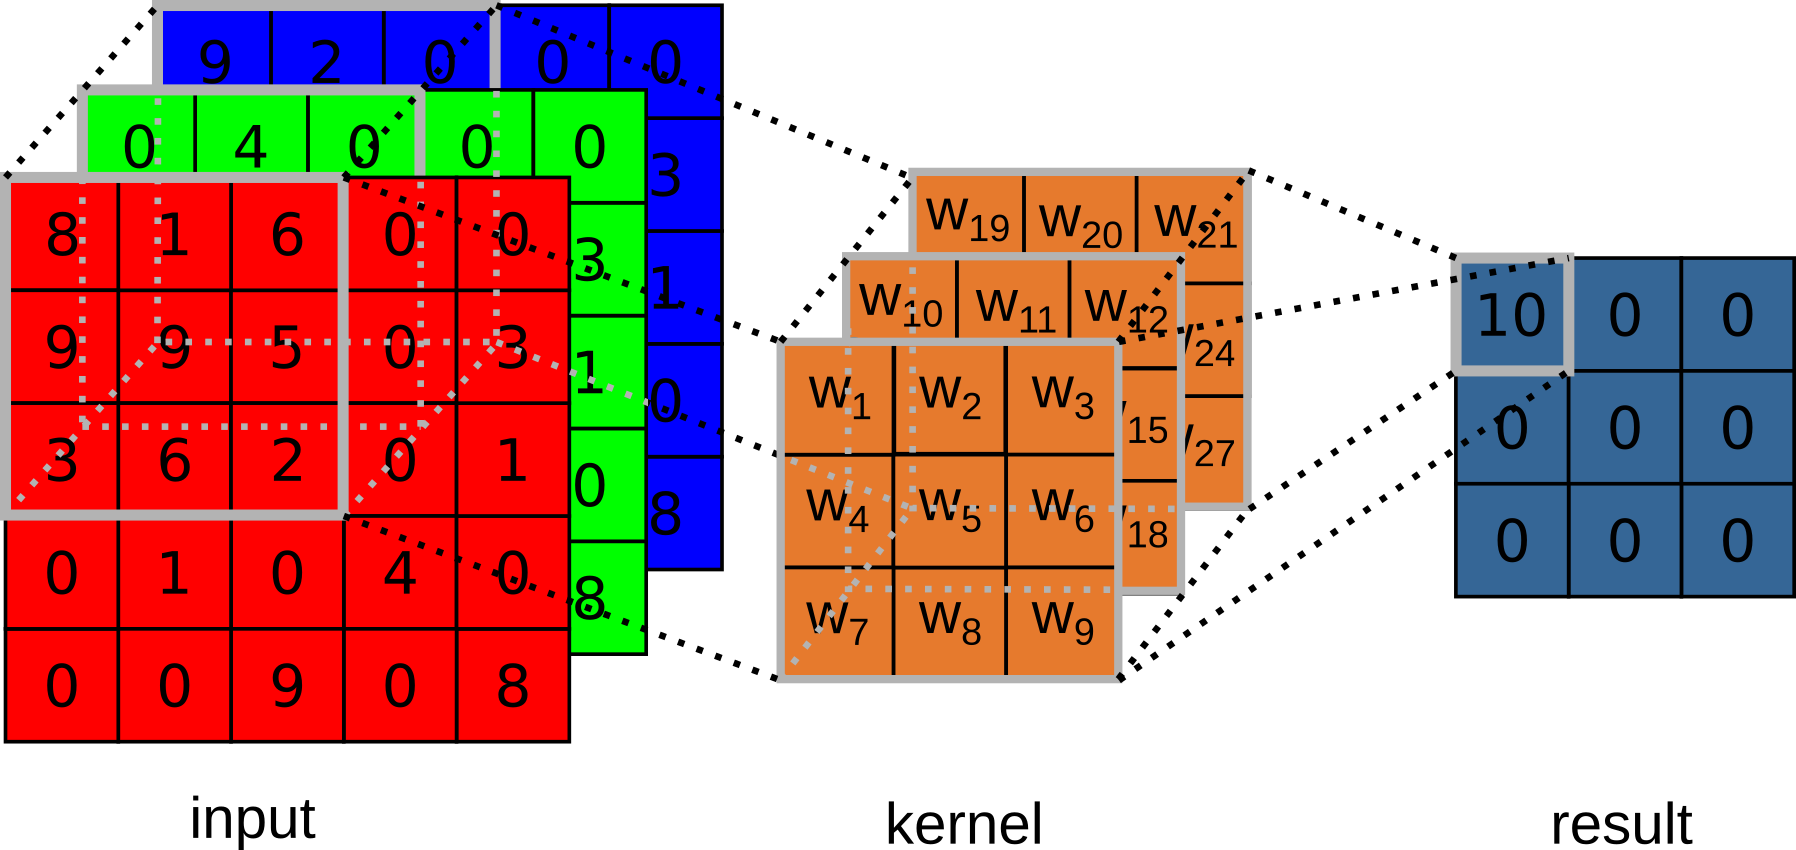
\includegraphics[scale=0.35]{images/figure118.png}
    \caption{Convolution of a 5x5x3 sized image with a 3x3x3 sized kernel and its result.}
    \label{fig:figure118}
\end{figure}

In Figure \ref{fig:figure119}, we have a representation of a convolution layer with more than one filter. For each one, we have an output and, consequently, we have in the final result a dataset where the number of depth layers (also known as feature map, illustrated by the three matrices in orange) will correspond to the number of filters applied to the input. This output can then be sent forward on the network, going through more convolutions and having more features extracted.

\begin{figure}
    \centering
    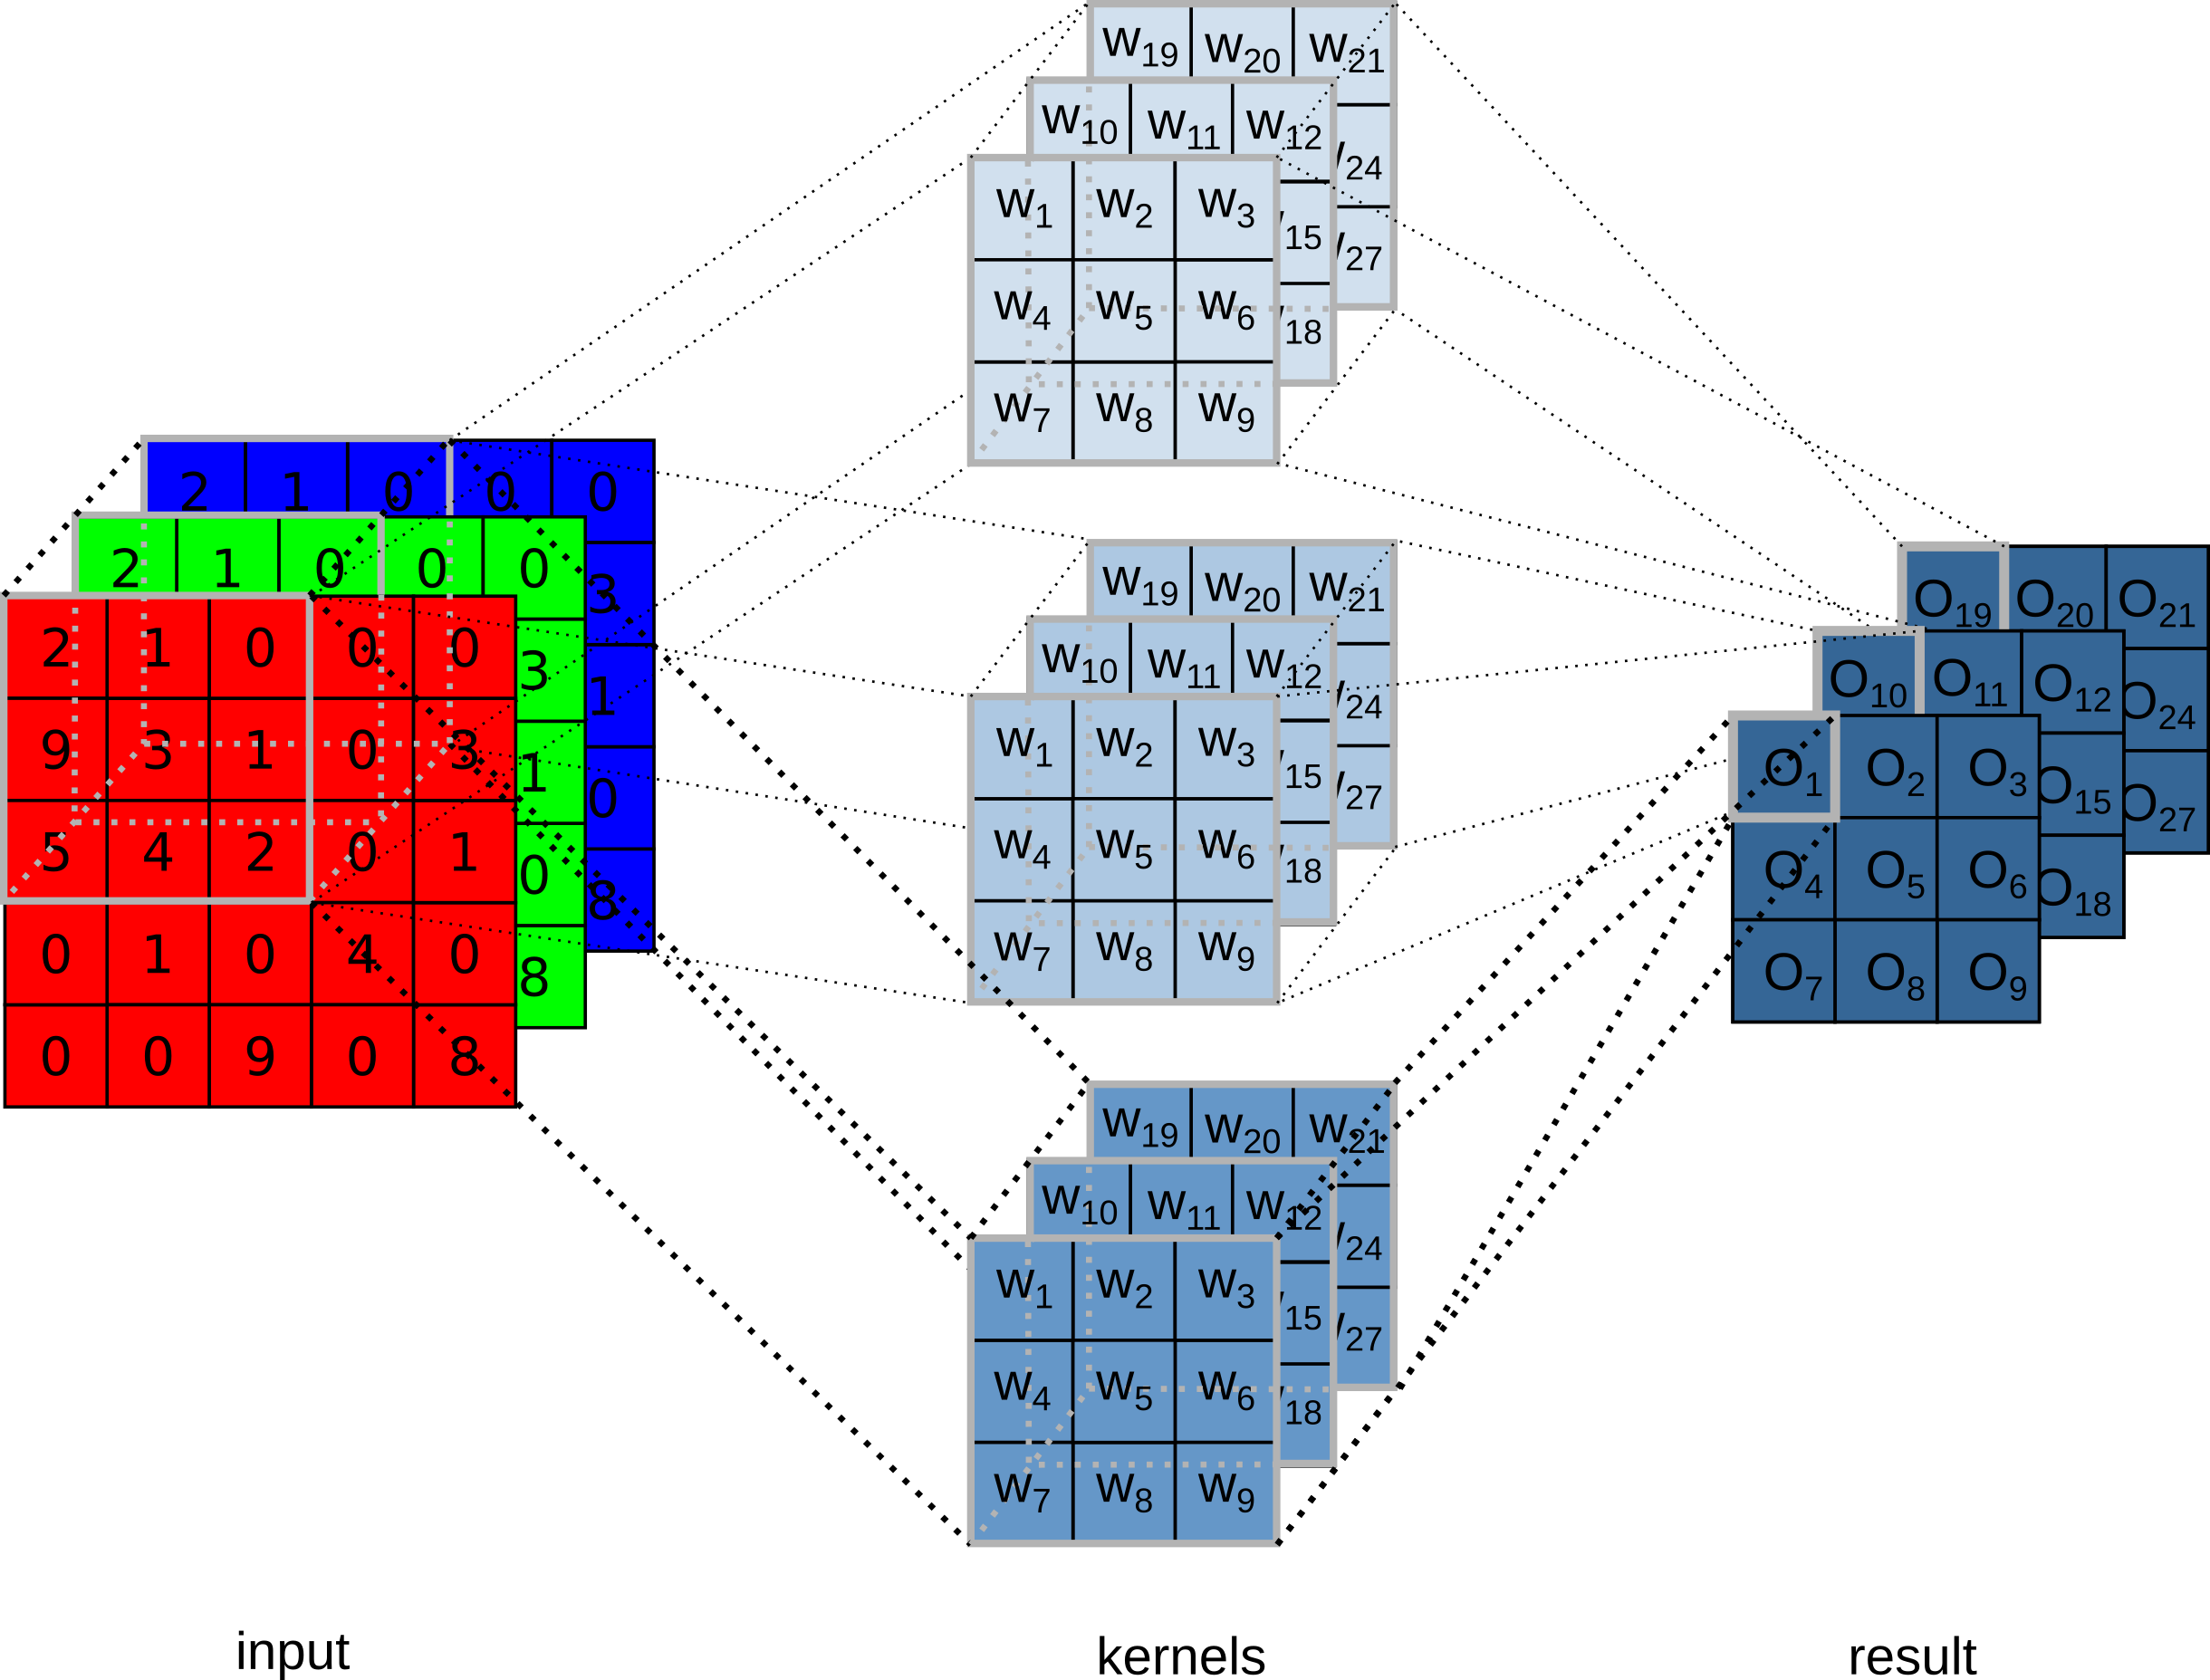
\includegraphics[scale=0.25]{images/figure119.png}
    \caption{Convolution of a 5x5x3 sized image with a 3x3x3 sized kernel and its result.}
    \label{fig:figure119}
\end{figure}

The two previous examples, Figures \ref{fig:figure117} and \ref{fig:figure119}, also serve to show us one of the features of convolution that make it a good choice for working with images, we call this feature sparse iterations (also known as sparse connectivity) \cite{goodfellow2016}. This attribute highlights the fact that each output unit, or pixel, is connected to only a fraction of the input units. In our previous example, each output is connected to a region of the 243 input pixels, 9x9x3. This is very useful, as our image can have millions of pixels, and using smaller sized kernels, we will be able to detect small features such as edges, corners, etc \cite{goodfellow2016}. In the convolution layers, the values that the network must learn are the values present in the filters, so that way we will have fewer parameters to learn and store. In a simple neural network, as we saw in the topic MLP network, an image at the input means that each pixel would be connected to each neuron in the next layer, thus resulting in an excessively large network.

Another important feature is the sharing of parameters, since the same filter is applied to different regions of the image using the same values, unlike a neural network without convolution layers, where we have a matrix with weights that are used for only one connection. The sharing of parameters gives us another feature, which is the invariance to translation, that is to say that if we move the position of an object in the input image, its representation will also be moved in the resulting image \cite{goodfellow2016}.

\subsection{Padding}

In the convolution examples, Figures \ref{fig:figure117} and \ref{fig:figure119}, we see that as we apply the kernel to the input image, the size of the output image is reduced. In fact, by convoluting a image of size $m x n$ with a filter of size $k_m x k_n$ the resulting image will have a height of $m-k_m+1$ and a length of $n-k_n+1$ . This type of convolution, where the resulting image is smaller, is often called “valid”.
If we want the output image to be the same size as the input image, we have to add more rows and columns to our image, this is known as padding. In this case, we use the formula  $m+2p-k_m+1$ and $n+2p-k_n+1$ where the padding represents. For example, in the previous Figures \ref{fig:figure117} and \ref{fig:figure119}, if we want an output equal in size to the input, we would have to use a padding of $6+2p-3+1=6p=1$.

\subsection{Stride}

The convolution examples we saw earlier used one-by-one displacement steps. But we can also use larger steps, as this reduces the computational cost of performing these steps at intervals. This clearly has an impact on the final result, decreasing its resolution, but in cases where we do not need to extract delicate features this becomes a good option \cite{goodfellow2016}.

When we use a stride value greater than one, this will also affect the output size, which will be governed by the following relationship \cite{adrian2017}:

\begin{equation}
\frac{m+2p-k_m}{s}+1 \  \times \ \frac{n+2p-k_n}{s}+1
\end{equation}

Where $m$ and $n$ are the image dimensions, p is the padding, $k_m$ and $k_n$ are the kernel dimensions and $s$ is the stride. In Figure \ref{fig:stride} we have an example with the steps of a convolution with stride=2 using a kernel of size 3 over an image of size 5 x 5 and padding=0.

\begin{figure}
    \centering
    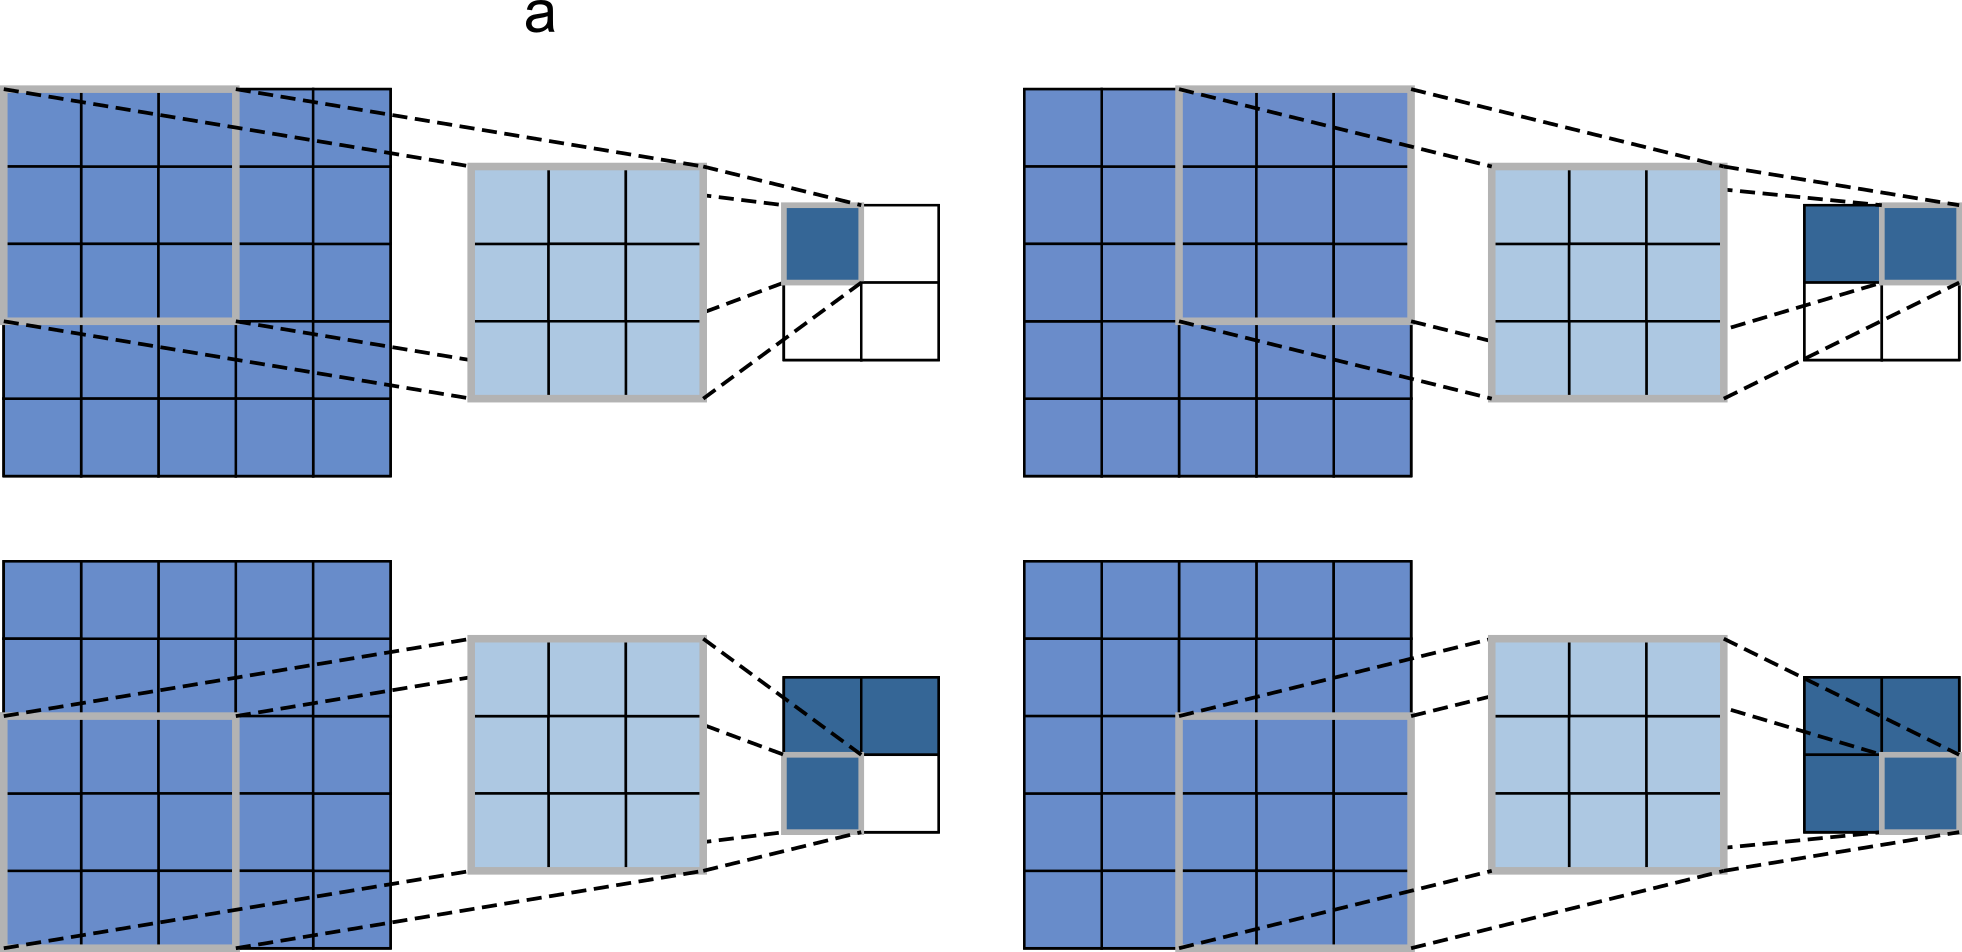
\includegraphics[scale=0.20]{images/stride.png}
    \caption{Example using stride bigger than 1.}
    \label{fig:stride}
\end{figure}

\subsection{Pooling Layer}

This is a very important layer, which aims to subsampling the image to reduce its size, and, consequently, reduce the total memory, processing and parameters needed, in addition to curbing the risk of overfitting \cite{geron2019}\cite{adrian2017}\cite{elgendy2020}.

As in convolution layers each output unit is connected to an input region, so we must also take into account size, stride and padding. But, unlike convolution, the “kernel,” or, in other words, the region that will connect us to the input, will have no weights but only perform one operation, the most common being the maximum or the average \cite{geron2019} .

In Figure \ref{fig:figure121}, we have an example of max pooling, where we can see how it works in steps (Figures \ref{fig:figure121}(a-d)). This example uses a region of 2 x 2 , which is very common \cite{adrian2017}, and stride=1.

\begin{figure}
    \centering
    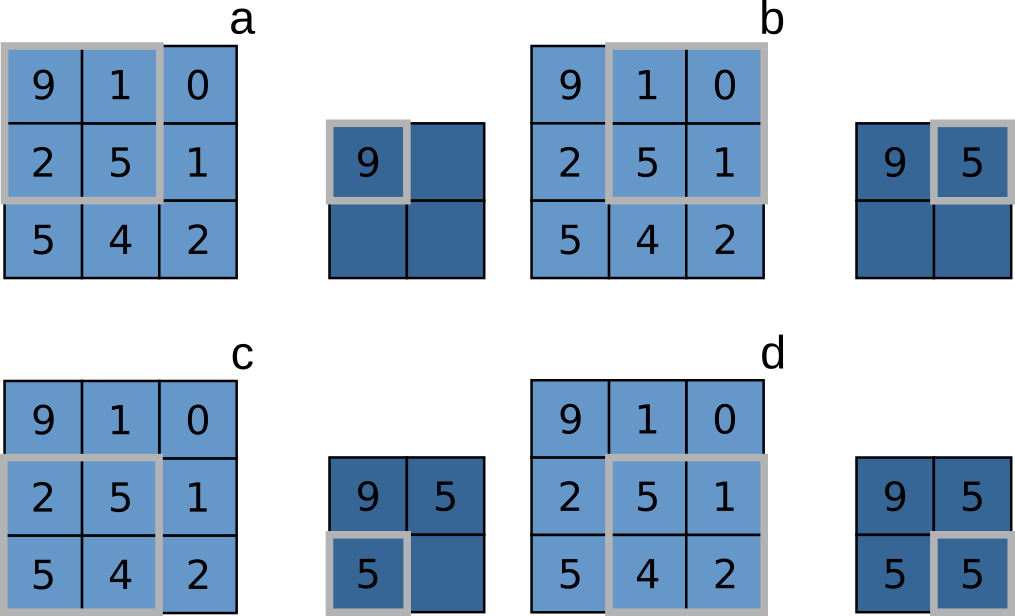
\includegraphics[scale=0.30]{images/figure121.png}
    \caption{Example of max pooling application.}
    \label{fig:figure121}
\end{figure}

In Figure \ref{fig:figure122}, we have another example of max pooling, but this time performed with a larger input, we can see that the operation is performed on each input layer of the object, and that its output contains the same number of layers as the input, which is what typically occurs in this type of operation \cite{geron2019}.

\begin{figure}
    \centering
    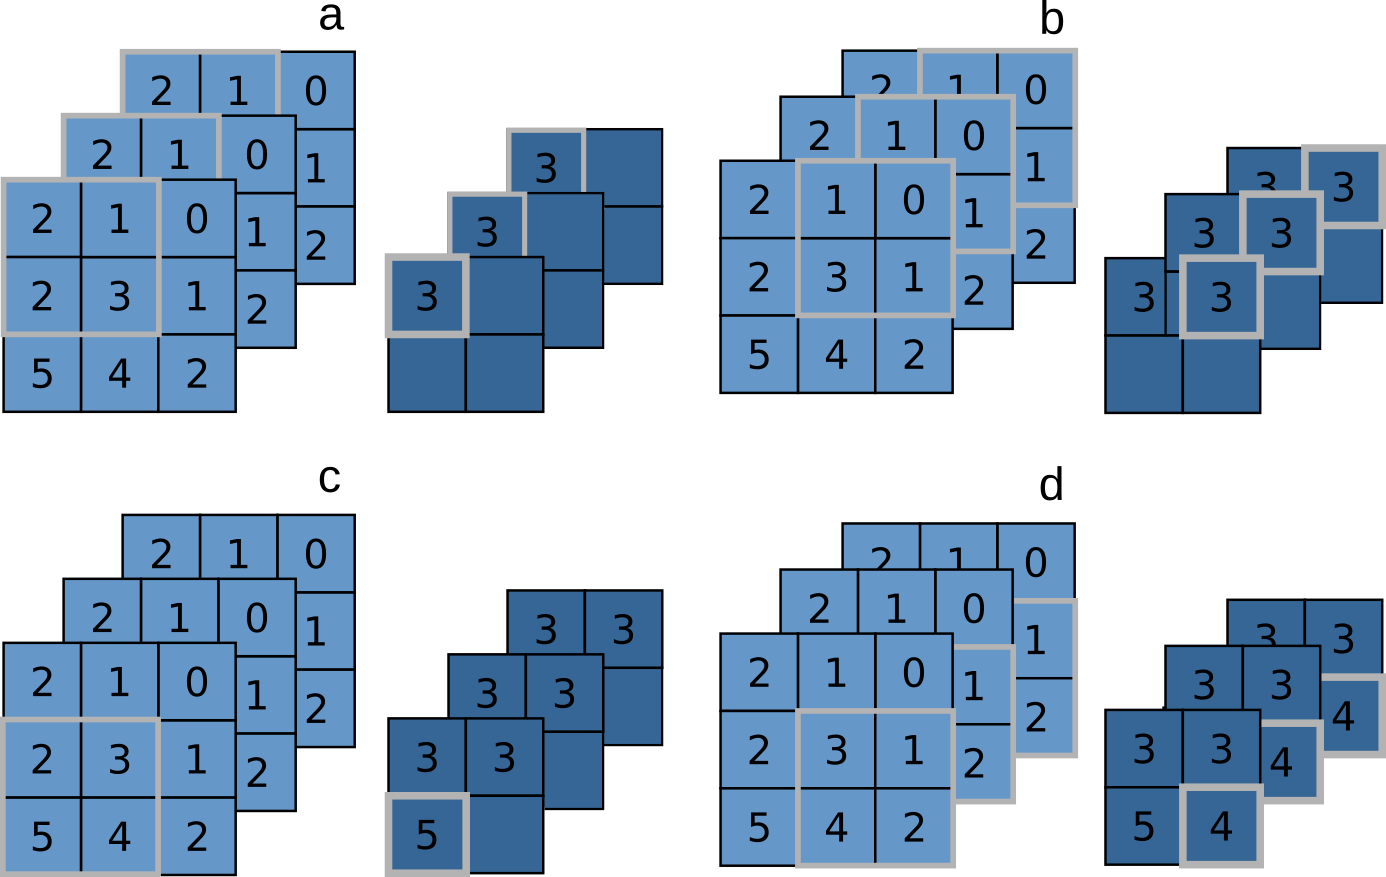
\includegraphics[scale=0.30]{images/figure122.png}
    \caption{Example of max pooling application in an image with more dimensions.}
    \label{fig:figure122}
\end{figure}

Although pooling is a very widespread technique, we can find networks where their authors preferred not to use pooling to perform subsampling, but to use convolution layers with higher stride and padding values to achieve this dimension reduction \cite{elgendy2020}\cite{adrian2017}. This way of working was proposed by Springenberg et al. in their 2014 article “Striving for Simplicity: The All Convolutional Net”, where they demonstrate that even networks without pooling layers can have good results in different databases, such as CIFAR-10 and ImageNet.

\subsection{Fully Connected Layers}

CNN's usually have several convolution layers followed by activation functions, which in turn are followed by pooling layers, and this process decreases the dimensions m x n and increases the depth, that is, the number of feature layers (known as feature maps ) \cite{elgendy2020}\cite{geron2019}. In Figure \ref{fig:figure123}, we have a representation of this process through the network topology. At the end of this network we have a large amount of layers with the characteristics extracted from the input image, and we need to use this information. In this same Figure, we can see that in the end we have fully connected layers, which is a regular neural network, an MLP \cite{elgendy2020}.

\begin{figure}
    \centering
    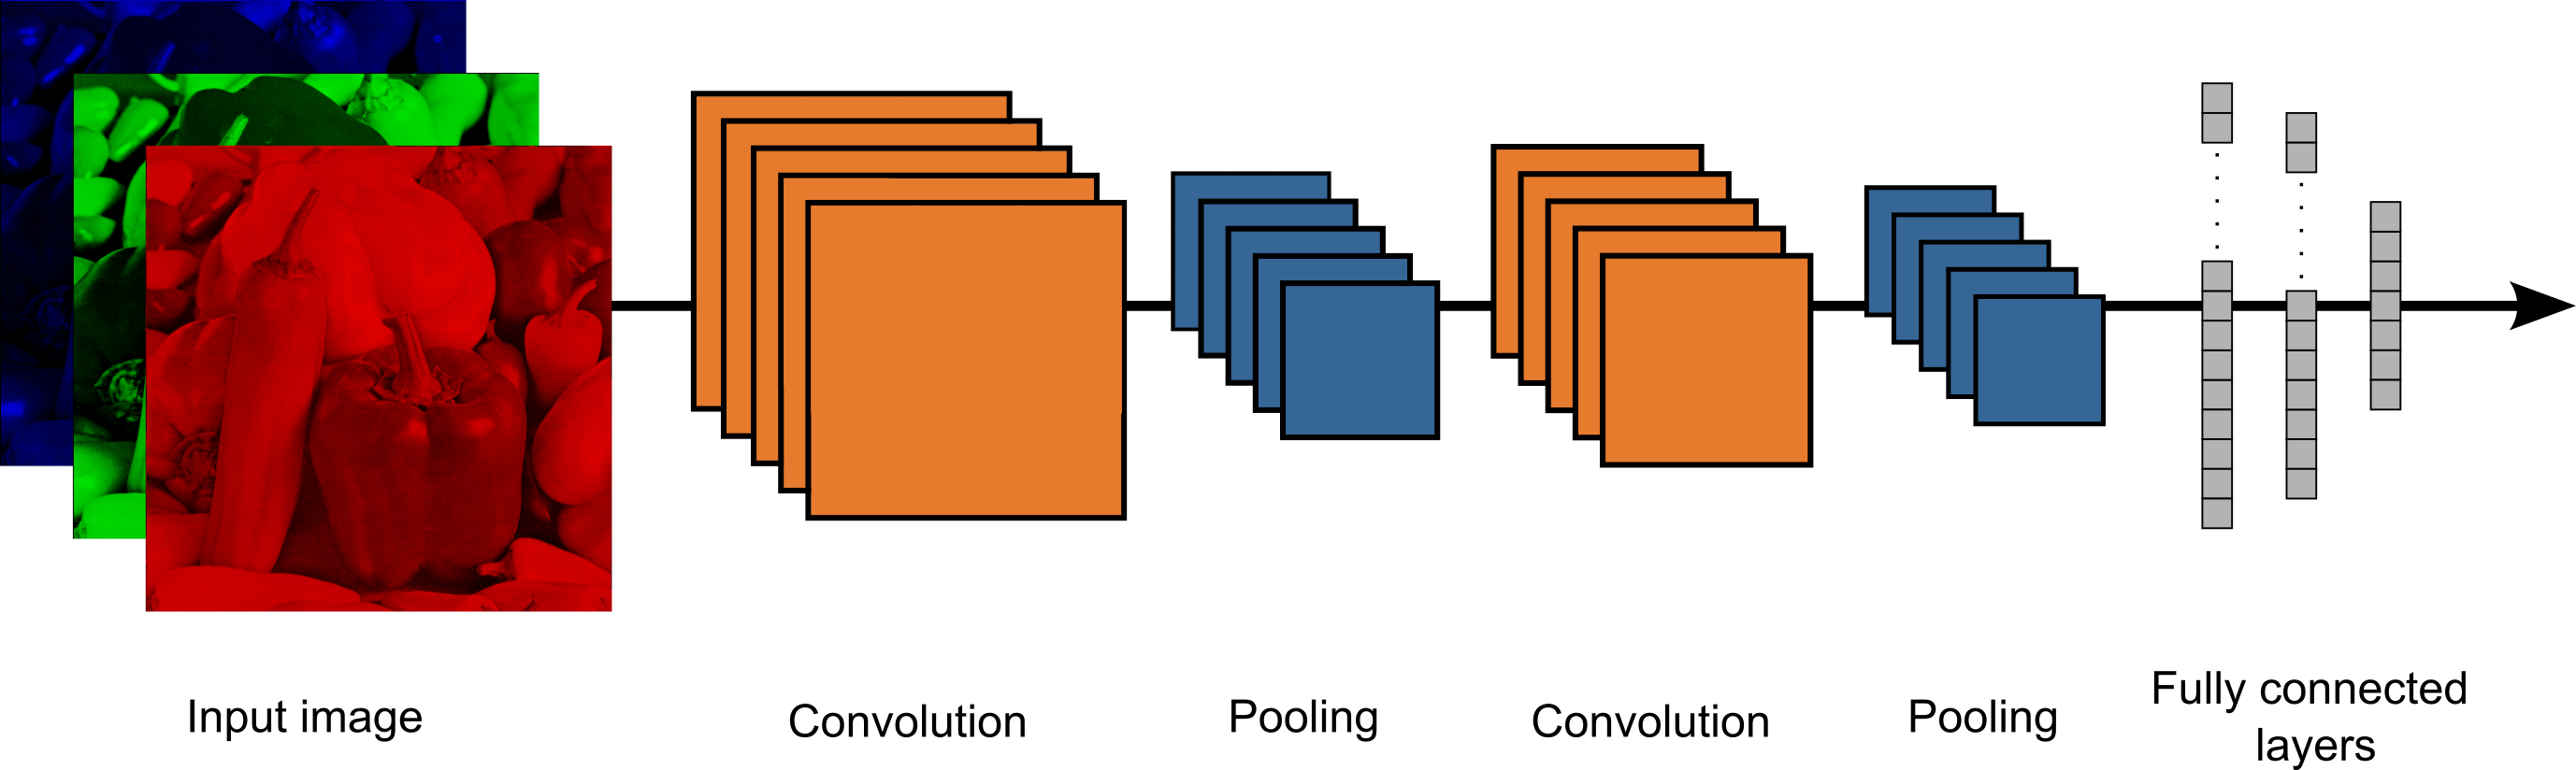
\includegraphics[scale=0.22]{images/figure123.png}
    \caption{Example of max pooling application  in an image with more dimensions.}
    \label{fig:figure123}
\end{figure}

In Figure \ref{fig:figure124} we have the representation of the use of the information abstracted from the image by the convolution layers. In this example, the data ends with a size of 7x7x64, that is, we have 64 feature maps with a size of 7x7. To provide this data to the full connected layer, we have to flatten these feature maps to a vector of dimensions 1x3136, that passes through the network and ends in the layer of Softmax, that produces the output vector.

\begin{figure}
    \centering
    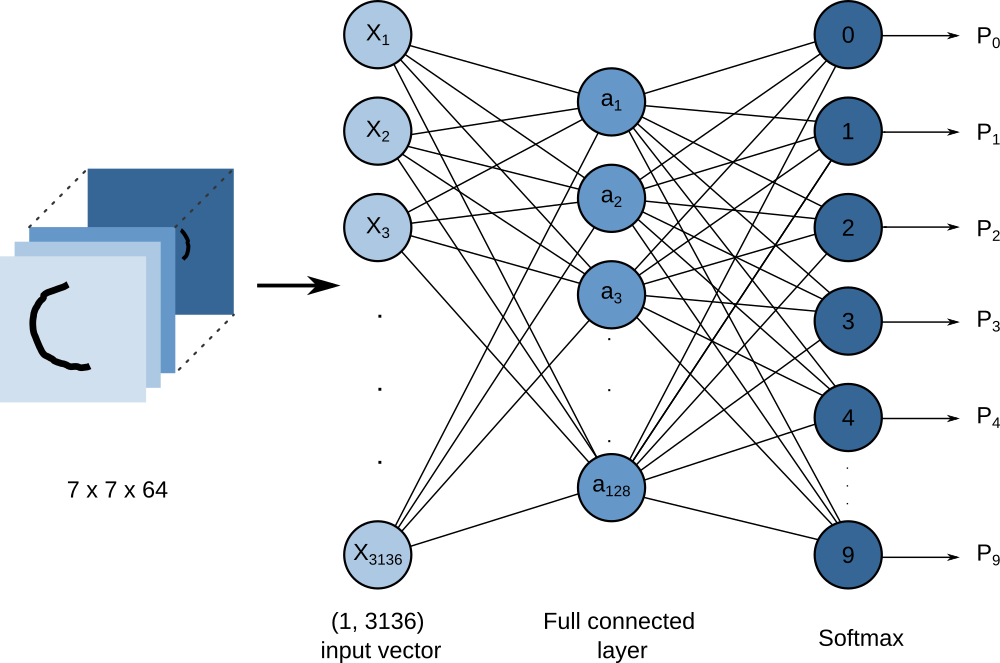
\includegraphics[scale=0.50]{images/figure124.png}
    \caption{Example of fully connected layers application in an image with more dimensions.}
    \label{fig:figure124}
\end{figure}


\subsection{Why Use Convolutions?}

So far we understand the building blocks of CNNs and the reasons they are used. The convolution operation is not only used because it is more efficient in image processing, but also because it is inspired by our own visual system.

Like many other neural network topologies, CNNs were bio-inspired by studies on the visual cortex of the human brain that began to take place since 1980 \cite{geron2019}, mainly from the work of David H. Hubel and Torsten Wiesel, where experiments conducted on animals allowed them to deduce the functioning of the structure of the visual cortex.

In short, light signals received by the retina are transmitted to the brain through the optic nerve, where they reach the primary visual cortex, which is mainly formed by two types of cells \cite{goodfellow2016}:

\begin{itemize}
\item \textbf{Simple cells}: these cells have behaviors that can be represented by linear functions in an image with small area known as the receptive field \cite{goodfellow2016,geron2019}. This type of cell inspired the simplest detector units on CNNs.
\item \textbf{Complex cells}: they also respond to features of the image, such as simple cells, but are invariant in position, that is, they do not make much distinction from where the feature appears. This type of cell inspired the pooling units \cite{goodfellow2016}.
\end{itemize}

Anatomically, the deeper we go into the layers of the brain, the more layers analogous to convolution and pooling are used, and we find more specialized cells that respond to specific patterns unaffected by input transformations. Until reaching these deeper layers, a sequence of detections followed by pooling layers is performed \cite{goodfellow2016}. 

\subsection{Classic CNNs}
\label{sec:architectures}

\subsubsection{LeNet} \label{lenet}

After studying the main building blocks of a CNN -- convolutional layers, pooling layers and fully connected layers -- it becomes easier to compare CNNs architectures and we can realize that even with the differences they present a pattern in the combination of layers. Typically, CNN architectures have an interleaved sequence of convolution layer, followed by a pooling layer, which repeats up to the edge of the network where there are some fully connected layers with similar structure to MLP networks. An example of this basic structure was shown in Figure \ref{fig:figure123}. 

Figure \ref{fig:lenet} illustrates a LeNet CNN. As the operations are carried out along this network, it is noticed that the feature maps are getting smaller and that the layers deeper, that is, the number of maps in the same layer increases. As the output layer usually presents itself as a vector of probabilities for each class, there is a transition from the representation of the data in maps to a vector, starting from the flattening process, which occurs before the first fully connected layer.

\begin{figure}[h]
    \centering
    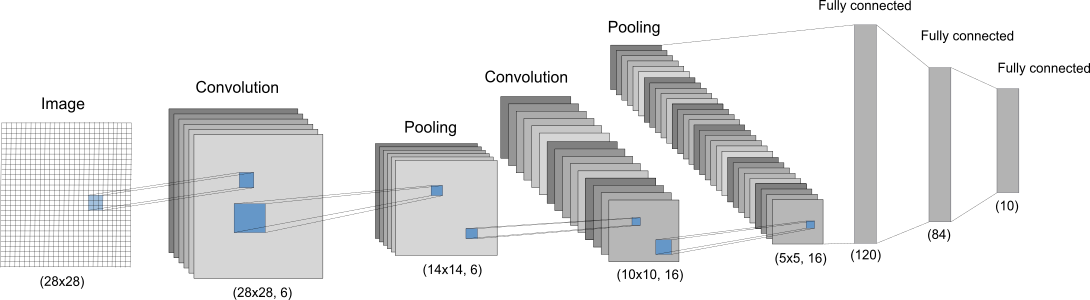
\includegraphics[scale=0.4]{"Part 3 - Learning Systems/Supervised Learning/Deep Learning/images/figure125.png"}
    \caption{ LeNet Convolutional Network - The input is an image of a handwritten number and the output a vector with the probability for each of the ten digits from 0 to 9 \cite{zhang2020dive}.}
    \label{fig:lenet}
\end{figure}

The LeNet network was one of the first CNNs that showed potential application in computer vision. The network was created by Yann LeCun in 1998 for the purpose of handwriting number recognition. LeNet was later adapted to recognize digits for ATM machine deposits, and there are still ATMs that run the code developed by Yann and his colleague Leon Bottou \cite{zhang2020dive}. The network was also widely used for digit recognition of the MNIST dataset \cite{geron2019}. %, this dataset was covered in topic \ref{backpropagation}.

In Figure \ref{fig:lenet}, we take as input a standard MNIST grayscale image, of size 28 x 28 pixels. In the general scheme of the LeNet network (Figure \ref{fig:lenet2}), we have a clearer view of the combination of layers, where after the input layer there are two convolutional layers, each followed by a pooling layer, and at the end there are three fully connected layers.

\begin{figure}
    \centering
    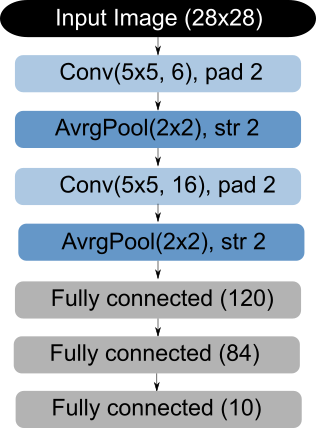
\includegraphics[scale=0.4]{"Part 3 - Learning Systems/Supervised Learning/Deep Learning/images/figure126.png"}
    \caption{ General diagram of layers in the LeNet network - Schematic of the LeNet network with the sequence of convolutional layers (“Conv”), pooling (“AvrgPool”) and fully connected layers \cite{zhang2020dive}.}
    \label{fig:lenet2}
\end{figure}

Each convolution layer uses a filter $5 \times 5$ and a sigmoid activation function (see the chapter about MLPs for a definition of activation functions). The first convolution layer has $6$ channels or maps, while the second one has $16$. The pooling operation involves a filter $2 \times 2$ that calculates the average, so it is identified as “AvrgPool”, and uses stride $str=2$, so that each map from the previous layer is reduced in a half along the width and height, eliminating $75\%$ of the activations. The size of the three fully connected layers are respectively $120$, $84$, and $10$. The last layer, “Fully connected(10)”, corresponds to the possible number of classes, in this case $10$ (digits from $0$ to $10$). The activation function in the last layer is a Gaussian function.

To understand the effects of each layer on the dataset, we present in Table \ref{table:tablelenet} the dimensions of the outputs of each layer. Table \ref{table:tablelenet} shows that from one convolution block to the other there is an increase in the number of channels (C) from 6 to 16, between the pooling layers these values are not changed, as the process only reduces the width (W) and height (H ) of the channels. In fully connected layers, the dimensions are reduced until the size of the number of classes is obtained.

\begin{center}
\begin{table}[]
\begin{tabular}{|l|c|c|c|c|c|}
\hline
\textbf{Layer}    & \textbf{\begin{tabular}[c]{@{}c@{}}Channel\\ (C)\end{tabular}} & \textbf{\begin{tabular}[c]{@{}c@{}}Size\\ (H,W)\end{tabular}} & \textbf{\begin{tabular}[c]{@{}c@{}}Filter\\ (K)\end{tabular}} & \textbf{\begin{tabular}[c]{@{}c@{}}Memory\\ (kB)\end{tabular}} & \textbf{Parameters} \\ \hline
Inputs            & 1                                                            & 28                                                              &                                                             &                                                                &                     \\ \hline
Convolutional 1   & 6                                                            & 28                                                              & 5                                                           & 18                                                             & 156                 \\ \hline
Avrg Pooling 1    & 6                                                            & 14                                                              & 2                                                           & 5                                                              & 0                   \\ \hline
Convolutional 2   & 16                                                           & 10                                                              & 5                                                           & 6                                                              & 2416                \\ \hline
Avrg Pooling 2    & 16                                                           & 5                                                               & 2                                                           & 2                                                              & 0                   \\ \hline
Flatten           & 400                                                          &                                                                 &                                                             & 1.6                                                            & 0                   \\ \hline
Fully Connected 1 & 120                                                          &                                                                 &                                                             & 0.5                                                            & 48120               \\ \hline
Fully Connected 2 & 84                                                           &                                                                 &                                                             & 0.3                                                            & 10164               \\ \hline
Fully Connected 3 & 10                                                           &                                                                 &                                                             & 0.04                                                           & 859                 \\ \hline
Total             &                                                              &                                                                 &                                                             & 33                                                             & 61706               \\ \hline
\end{tabular}
\caption{LeNet Layer Settings, Parameters and Information - Summary of LeNet's main layer settings such as number of channels and filter size. Display an estimate of the number of parameters and the amount of memory to train the network.}

\label{table:tablelenet}
\end{table}
\end{center}

It is common in CNN's networks that the number of channels practically doubles after a pooling layer since there is a reduction by half in the dimensions of the maps. Thus, it is possible to increase the number of maps, making it more sensitive to identify low-level features such as borders and textures, without drastically increasing the number of parameters and computational resources \cite{zhang2020dive}. As the first convolution layer applies  $\text{padding}=2$, the maps maintain the same dimension in the output as the original image ($28 \times  28$), however the second layer does not have padding, which reduces the width and height of the maps by $4$ pixels.

Over the years, variations of this model have emerged and the most evident difference between the networks is the number of layers, which has increased over the years, making the networks deeper. When increasing the number of layers it was noticed that the performance of the networks tended to improve, however some limitations emerged. The greater the amount of data, the more computational memory is required, and this capacity depends on hardware requirements.

To assess the amount of memory used in training the LeNet network, we will use an approximate calculation based on the amount of output elements in each layer. The number of elements is multiplied by the number of bytes needed to store each element \cite{johnson2019}. Considering that floating point data occupy $32 \text{ bits}$, therefore  $4 \text{ bytes}$ per element, to facilitate the visualization of the results, the measure kilobyte (kB) is used, and for this reason they were divided by the factor 1024 since  $1 \text{ kB} = 1024 \text{ B}$ . In Equation \ref{qtdMemoria}, we exemplify the calculation of the amount of memory for the first convolution layer of the LeNet network:


\begin{equation}
\begin{split}
\text{Amount of memory }& = \text{CxHxW}\\ 
&= 6 \times  28 \times  28\\
&= 4704 \text{ output elements}\\
&= 4704 \times 4 \text{ bytes} = 18816 \text{ bytes}\\
&= 18.38 \text{ kilobytes}
\end{split}
\label{qtdMemoria}
\end{equation}

The C parameter identifies the number of channels or maps of the layer and the term H and W, the height and width of the layers output element, respectively. As shown in Equation \ref{qtdMemoria} and Table \ref{table:tablelenet}, the approximate amount of memory for the first layer is $18 \text{ kB}$, and in total for the network $33 \text{ kB}$. The first layers tend to need more memory due to the larger dimensions (W and H) of the channels \cite{johnson2019}.

Increasing the number of layers also requires that more parameters be learned, which affects both the training time and its performance, because if there is not an adequate optimization of the parameters, the probability of overfitting can be higher \cite{elgendy2020}. To approximately determine the number of parameters related to each layer, the weights related to the filters of each map were considered, calculated as the product between the filter dimensions ($\text{K x K}$), the number of input element channels and the number of output channels of the layer \cite{johnson2019}. The biases associated to each output channel were also considered as parameters. On fully connected layers, the number of parameters is determined as the product of the number of input elements and the number of output elements of the layer plus the number of biases. Equation \ref{calcConvInfos} exemplifies the calculations for the first convolution layer:

\begin{equation}
\begin{split}
  \text{Weights} &= \text{C}_\text{output} \times  \text{C}_\text{input} \times  \text{K} \times  \text{K}\\ 
  &= 6\times 1 \times  5 \times  5\\
  &= 150\\\\
  \text{Bias} &= 6\\\\
  \text{Parameters} &= \text{Weights} + \text{Bias}\\
  &= 150 + 6\\
  &= 156
\end{split}
\label{calcConvInfos}
\end{equation}

Considering that the filter in the first layer is of size $5\times 5$, that the input has only 1 channel and that there are 6 channels in the convolution layer, the first convolution layer considers approximately 156 parameters. In Table \ref{table:tablelenet}, there is also the number of parameters related to each layer and the approximate total of parameters for the LeNet network is 61706. As the number of channels in the convolution layer increases, more parameters are needed. In general, most parameters are due to fully connected layers due to the greater number of connections \cite{johnson2019}.

\subsubsection{AlexNet}

Currently there are several CNNs network architectures used for applications in computer vision. The evolution of these networks can be seen in the results of the ImageNet Large Scale Visual Recognition Challenge (ILSVRC) competition. The main objective of the competition was to evaluate algorithms for object detection and image classification. The first edition of the competition, in 2010, involved 1.2 million images for training, being 1000 categories of objects. In the first two years of competition, CNNs networks weren't yet in 1st place, however, from on 2012 CNNs models started to lead the competition \cite{imagenet2020}. The progress of the networks can be evaluated based on the error rate of the models, which in seven years dropped from approximately $26\%$, in the second year of the competition, to $2.3\%$ in the last edition of the competition in 2017 \cite{johnson2019}, as shown in the graph in Figure \ref{fig:imagenet}.


\begin{figure}
    \centering
    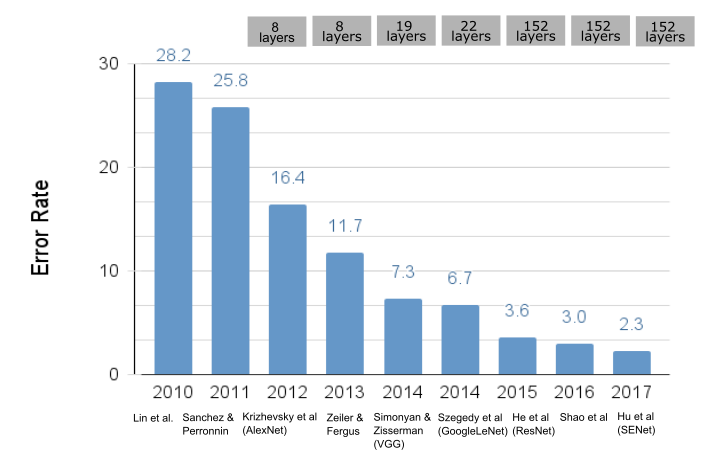
\includegraphics[scale=0.4]{"Part 3 - Learning Systems/Supervised Learning/Deep Learning/images/figure127.png"}
    \caption{ Error rate of the best performing models in the ImageNet competition - The performance of the models in the ImageNet Large Scale Visual Recognition Challenge (ILSVRC) competition was mainly evaluated by the error rate. The graph shows the models that won in each edition of the competition, which ran from 2010 to 2017, and also networks that became popular such as VGG \cite{johnson2019}.}
    \label{fig:imagenet}
\end{figure}

To learn a little about the different architectures of CNNs networks and notice some differences, and structures that performed well and are still adopted by recent architectures, we will highlight below three additional architectures that become well known and had prominence in the competition. The AlexNet network was the first CNN to win the ImageNet competition in 2012 with an error rate of $16.4\%$. The VGG network did not lead the competition in 2014, but it is one of the models with great popularity. In 2014, the CNN GoogLeNet won the competition and served as inspiration for the Inceptions networks. %The Residual network (ResNet) in 2015, in addition to taking advantage of the higher performance techniques of other networks, also carried an approach that made it possible to increase its depth to more than 100 layers.

The AlexNet network was developed by Alex Krizhevsky, Ilya Sutskever, and Geoffrey Hinton \cite{geron2019}. This network is very similar to LeNet, but has more layers. Because it is a deeper network, requiring more memory, the original network had to be physically distributed between two 3GB GPUs  \cite{krizhevsky2012}. In this way, the network was drawn as in Figure \ref{fig:alexnet}, with a dual data stream structure so that each GPU would receive half of the model.

\begin{sidewaysfigure}[p]
    \centering
    \vspace{10cm}
    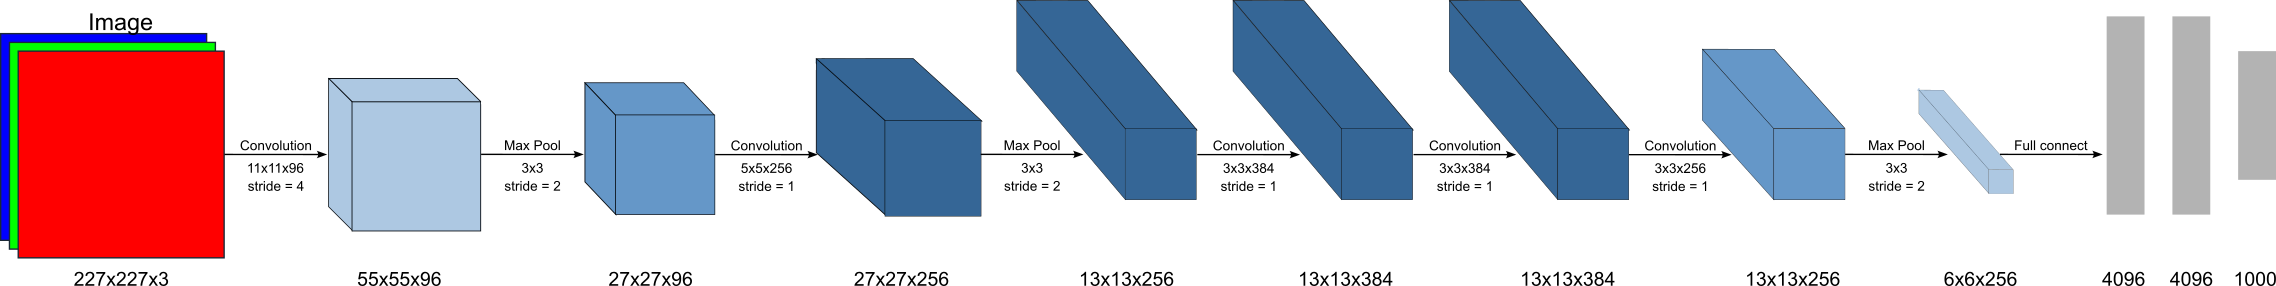
\includegraphics[scale=0.4]{"Part 3 - Learning Systems/Supervised Learning/Deep Learning/images/figure128.png"}
    \caption{ AlexNet network architecture - represented as the combination of two identical networks, as originally the training would occur with the distribution of data between two GPU's \cite{krizhevsky2012}.}
    \label{fig:alexnet}
\end{sidewaysfigure}

As depicted in Figure \ref{fig:lenetalexnet}, AlexNet has 5 convolution layers, with the first three followed by pooling layers. The most aparent difference between the AlexNet and LeNet architectures are the three additional convolution layers in the AlexNet network, which are followed one after the other with no layer pooling between them. As the input images are bigger than the MNIST dataset approached in the example LeNet network, the input convolution filters are bigger ($11\times 11$) and stride $\text{str} = 4$ is used. In the second convolution layer, the filters have size $5\times 5$, and in the other convolution layers filters $3\times 3$ are used.

With the discovery that ReLU's activation functions in the convolution layers and that maxpooling improve the performance of networks, most models were built using these functions \cite{zhang2020dive}. Maxpooling filters of size $3\times 3$ and stride $\text{str} = 2$ scale down channels based on the largest value of the receive field. With the exception of the first layer, all other convolution layers are padded so that the dimension of the channels is not changed after the convolutions.

The last three layers are fully connected and have sizes 4096, 4096 and 1000, respectively. The output layer has dimension 1000 due to the number of possible classes of ImageNet competition and the activation function is Softmax.

\begin{figure}[h]
    \centering
    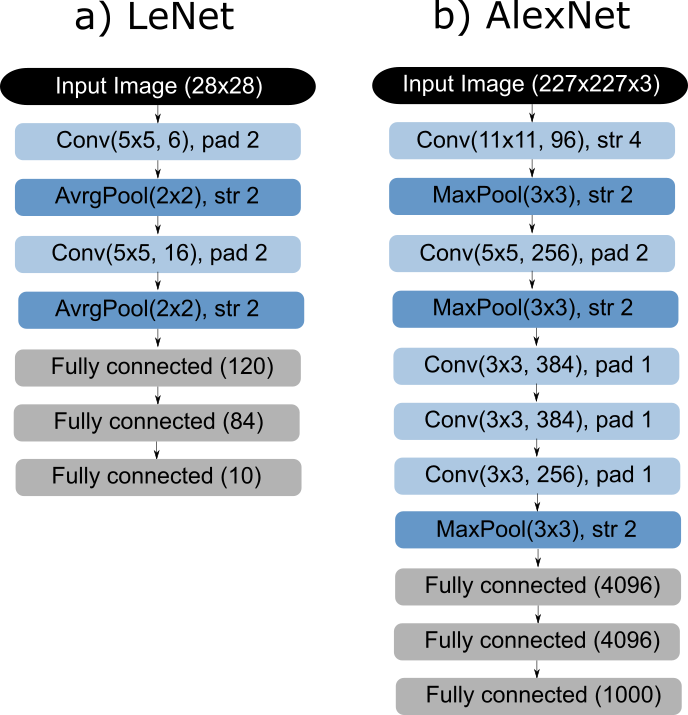
\includegraphics[scale=0.4]{"Part 3 - Learning Systems/Supervised Learning/Deep Learning/images/figure129.png"}
    \caption{ Comparison of AlexNet and LeNet networks. (a) LeNet Network and (b)  AlexNet Network. These general layer schemes show that the main difference of networks is that AlexNet is deeper, with three more convolution layers than LeNet \cite{zhang2020dive}.}
    \label{fig:lenetalexnet}
\end{figure}

The same pattern for the dimensions of the layer output elements seen in LeNet is seen in Table \ref{table:tablealexnet} for the AlexNet network. While the size of the channels decreases from one convolution layer to another, the number of channels increases, with 96 in the first, followed by 256, 384, 384 and 256. After the flatten process, the dimension of the layers is reduced until it is established the size of the prediction classes vector.

By comparing the amount of memory and the approximate number of parameters as described in the subsection \ref{lenet} it is observed that the amount of memory required increases and the number of parameters also increases. Approximate calculations indicate that while the memory required for training the LeNet network would be approximately $33 \text{ kB}$, for AlexNet it would be approximately $3\text{ GB}$. The number of parameters calculated for LeNet was 62 thousand and for AlexNet 62 million.  Generally in both models, the first layers require more memory, while the fully connected layers need more parameters.

\begin{center}
\begin{table}[]
\begin{tabular}{|l|c|c|c|c|c|}
\hline
\textbf{Layer}    & \textbf{\begin{tabular}[c]{@{}c@{}}Channel\\ (C)\end{tabular}} & \textbf{\begin{tabular}[c]{@{}c@{}}Size\\ (H,W)\end{tabular}} & \textbf{\begin{tabular}[c]{@{}c@{}}Filter\\ (K)\end{tabular}} & \textbf{\begin{tabular}[c]{@{}c@{}}Memory\\ (kB)\end{tabular}} & \textbf{Parameters} \\ \hline
Inputs            & 3                                                              & 227                                                           &                                                               &                                                                &                     \\ \hline
Convolutional 1   & 96                                                             & 55                                                            & 11                                                            & 1134                                                           & 35                  \\ \hline
Max Pooling 1     & 96                                                             & 27                                                            & 3                                                             & 273                                                            & 0                   \\ \hline
Convolutional 2   & 256                                                            & 27                                                            & 5                                                             & 729                                                            & 615                 \\ \hline
Max Pooling 2     & 256                                                            & 13                                                            & 3                                                             & 169                                                            & 0                   \\ \hline
Convolutional 3   & 384                                                            & 13                                                            & 3                                                             & 254                                                            & 885                 \\ \hline
Convolutional 4   & 384                                                            & 13                                                            & 3                                                             & 254                                                            & 1327                \\ \hline
Convolutional 5   & 256                                                            & 13                                                            & 3                                                             & 169                                                            & 885                 \\ \hline
Max Pooling 3     & 256                                                            & 6                                                             & 3                                                             & 36                                                             & 0                   \\ \hline
Flatten           & 9216                                                           &                                                               &                                                               & 36                                                             & 0                   \\ \hline
Fully Connected 1 & 4096                                                           &                                                               &                                                               & 16                                                             & 37753               \\ \hline
Fully Connected 2 & 4096                                                           &                                                               &                                                               & 16                                                             & 16781               \\ \hline
Fully Connected 3 & 1000                                                           &                                                               &                                                               & 4                                                              & 4097                \\ \hline
Total             &                                                                &                                                               &                                                               & 3090                                                           & 62378               \\ \hline
\end{tabular}
\caption{AlexNet Layer Settings, Parameters, and Information - Summary of settings for the main AlexNet layers, such as number of channels and size of filters. Display an estimate of the number of parameters and the amount of memory to train the network.}

\label{table:tablealexnet}
\end{table}
\end{center}

\subsubsection{VGG} \label{vgg}

The VGG network was conceived by the members of the Visual Geometry Group (VGG) at Oxford University by researchers Karen Simonyan and Andrew Zisserman \cite{zhang2020dive}. Compared to the two previous architectures LeNet and AlexNet, VGG adopts principles to establish the structure of the network, which allowed the construction of deeper models \cite{zhang2020dive}. Another characteristic of VGG is the block structure in the part of the network with the convolutional layers, in which each block presents convolutional layers in sequence and at the end a pooling layer. While the AlexNet model, in Figure \ref{fig:alexnetvgg}, presents 5 convolutional layers, the VGG presents 5 blocks with a variable number of convolution layers, but in general the first blocks have fewer layers. Like AlexNet, at the edge of the network there are three fully connected layers, with equal dimensions on both models, and a Softmax activation function at the output.

In Figure \ref{fig:alexnetvgg}, there is a representation of the VGG architecture with 16 layers, in which the first two blocks have two convolutional layers and the last three blocks have three convolutional layers. The convolution layers double in size with each block, with each layer in the first block having 64 channels, 128 channels in the next, and so on up to 512 in the last block. The use of the ReLu activation function in the convolution layer and maximum value pooling are strategies that performed well in AlexNet and continued in other models, such as in VGG.

\begin{figure}[h]
    \centering
    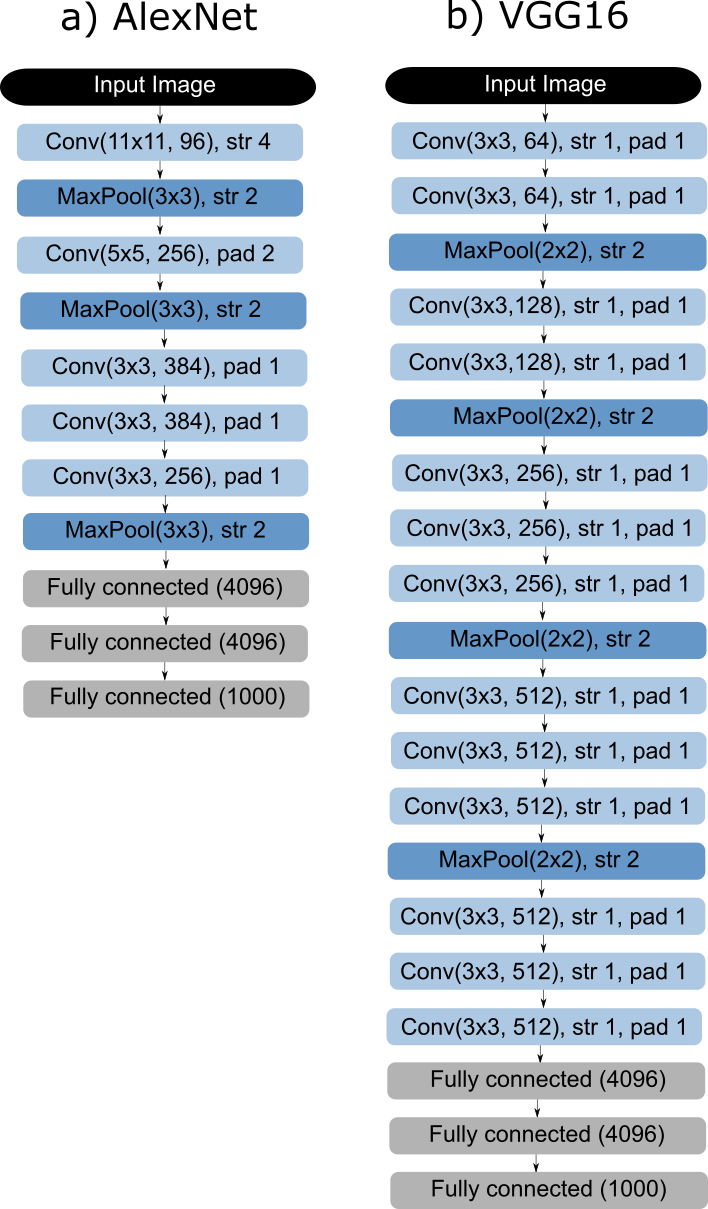
\includegraphics[scale=0.4]{"Part 3 - Learning Systems/Supervised Learning/Deep Learning/images/figure130.png"}
    \caption{ Comparison of VGG and AlexNet networks - Comparison of VGG and AlexNet networks based on the general structure of the layers. While the final part of the networks is similar in relation to the fully connected layers, the VGG differs in that it is deeper and presents a pattern of convolutional layers organized in blocks  \cite{johnson2019}.}
    \label{fig:alexnetvgg}
\end{figure}

In LeNet and AlexNet networks, it is usually necessary to individually select several hyperparameters\footnote{Hyperparameters are parameters that need to be pre-defined, as opposed to learned by the model.}. For example, in the convolution layers, the number of channels, size of filters, padding and stride are adjustable. In the pooling layer, the hyperparameters are the filter and stride size. In general, these two networks do not provide a general guide on how to select the parameters. VGG's core design principles state that all convolution filters are $3\times 3$ with stride $\text{str} = 1$ and padding $\text{pad} = 1$, and that maxpooling filters are $2\times 2$ with $\text{str} = 2$. After each pooling layer, the number of channels doubles in the convolution layer. The idea of fixing the size of convolutional filters came from the perception that the combination of two filters $3\times 3$ presents a receptive field equivalent to one filter $5\times 5$, and that three filters $3\times 3$ perform similar to one of $7\times 7$ \cite{elgendy2020}. Fixing the size of filters and their stride $\text{str} = 1$ and $\text{pad} = 1$ establishes that the dimension of the channels does not change between the convolutional layers, so the only hyperparameter that needs to be optimized is the number of layers in each block.

By using filters $3\times 3$, which are smaller, but in greater quantity than those used in AlexNet ($11\times 11$ and $5\times 5$), more nonlinearity is included, allowing the network to learn more low-level features \cite{elgendy2020}. Increasing the depth of the network with more layers of convolution adds more non-linear activation functions. Even being deeper networks, this strategy of using smaller filters reduces the number of parameters. Considering that two layers in sequence have C channels each, when using two filters $3\times 3$, the total number of parameters is $2\times 3\times 3\times \text{C}^2 = 18\text{C}^2$, which is smaller number when compared to the scenario of a single filter $5\times 5$ with $25\text{C}^2$ parameters \cite{johnson2019}.

Of course, doubling the number of channels between blocks should make the number of parameters grow quickly, and that's why maxpooling filters have been standardized to reduce the dimensions of the channels by half. By controlling the number of activations that pass to the next layers, it is possible to keep the number of operations approximately constant. Superficially evaluating that the number of operations is given as the total amount of multiplications and additions, we can calculate for each layer as the product of four parameters in Equation \ref{numOperacoes} \cite{johnson2019}: filter size($\text{K x K}$), input channel dimensions ($\text{H x W}$), quantity of input channels ($\text{C}_{\text{input}}$) and output channels ($\text{C}_{\text{output}}$).

\begin{equation}
\begin{split}
  \text{Number of operations} &= \text{Number of output elements x Operations by output element}\\
  &= (\text{C}_{\text{output}} \text{ x H x W}) \times  (\text{C}_{\text{input}} \text{ x K x K})\\
  &= (2\text{C x HW}) \times  (\text{2C x 3 x 3})\\
  &= 36 \text{HWC}^2
\end{split}
\label{numOperacoes}
\end{equation}

In the case of two convolution layers with filters $3\times 3$ and separated by a pooling, reducing by half the size of the channels ($\text{2H x 2W} \rightarrow \text{H x W}$) and doubling the number of channels ($\text{C} \rightarrow \text{2C}$), the number of weights increases from $9\text{C}^2$ to $36\text{C}^2$, but the number of operations remains at $36\text{HWC}^2$.

\subsubsection{GoogLenet and Inception} \label{inception}

By following the evolution of CNNs, we can see that the main strategy to increase the performance in the classification of images was to increase the number of layers that keep the weights of the networks. AlexNet and VGG-16 networks were developed with 8 and 16 layers, respectively. As the networks get deeper, the dilemma of how to make the algorithms more efficient arose, since more layers meant more parameters and operations, requiring more computational resources. Comparing the networks in Figure \ref{fig:neuralevolution}, it is possible to verify the accuracy of the networks, the number of parameters and the number of operations. It appears that for the VGG-16 network to achieve better results than the AlexNet network, it was necessary to more than twice the number of parameters, from approximately 65 million on AlexNet to just over 130 million on VGG-16.

In the 2014 ImageNet competition, a Google research group led by Christian Szegedy proposed the GoogLeNet architecture that should both ensure good performance and be more efficient than existing models \cite{geron2019}. The model not only won the competition but also met their requirements, as even being a network with 22 layers, more than the VGG-16, it used 12 times less parameters than VGG, 13 million instead of 138 million \cite{elgendy2020}.

\begin{figure}
    \centering
    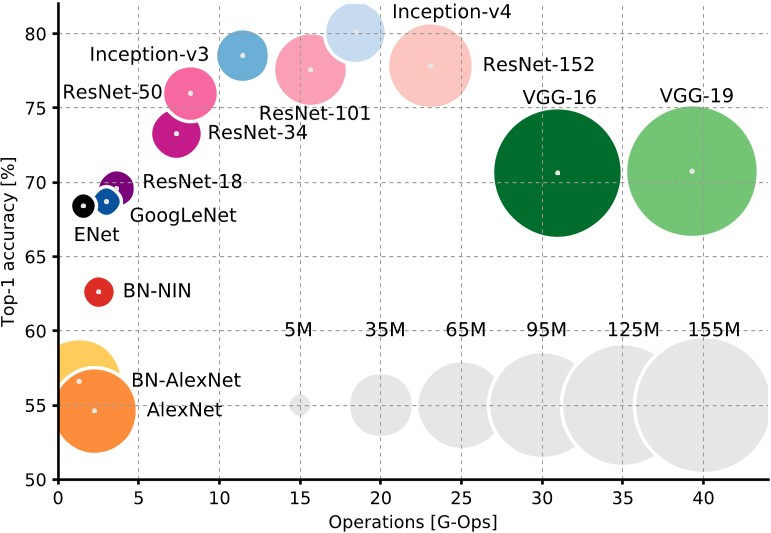
\includegraphics[width=\textwidth]{"Part 3 - Learning Systems/Supervised Learning/Deep Learning/images/figure131.jpg"}
    \caption{ CNN's neural networks evolution graph - Network performance is evaluated by accuracy versus the number of operations required for a single forward step. The radius of the circles is proportional to the number of parameters, with the legend in the lower right corner indicating a reference from $5\times 10^6$ to $155\times 10^6$ \cite{canziani2016}.}
    \label{fig:neuralevolution}
\end{figure}

To understand the GoogLenet network we can divide it into three parts (Figure \ref{fig:googlenet}), in the first part, the input layers are similar to the AlexNet and VGG networks, in the second part, there are the inception blocks characteristic of this network, and the last part refers to the classification structure. The first part contains two blocks with a sequence of convolutional layers followed by pooling $3\times 3$. In the first block, there is only a convolution layer $7\times 7$, with stride $\text{str} = 2$ and padding $\text{pad}= 3$, and a pooling layer with $\text{str} = 2$. At the end of these two layers, the element has 64 channels and was reduced by 4 in its dimension (H and W). In the second block, there are two convolution layers, the first with a filter $1\times 1$ and 64 channels and the second $3\times 3$ with 192 channels, and only the pooling $3\times 3$ at the end of the block changes the dimensions of the channels in half.

The main role of these two blocks is to reduce considerably the dimensions of the image, since most of the memory required is due to the first layers \cite{johnson2019}. Whereas, at this stage, there is an 8-fold reduction in image dimensions, an entry $224\times 224$ when reducing to approximately $28\times 28$ use approximately $7.5 \text{ MB}$ memory while the same reduction in VGG-16 needs $42.9 \text{ MB}$, almost $6$ times more than GoogLenet \cite{johnson2019}. Also, when passing a smaller image to the next layers, the number of operations and the number of parameters to train the network are also reduced.

\begin{figure}
    \centering
    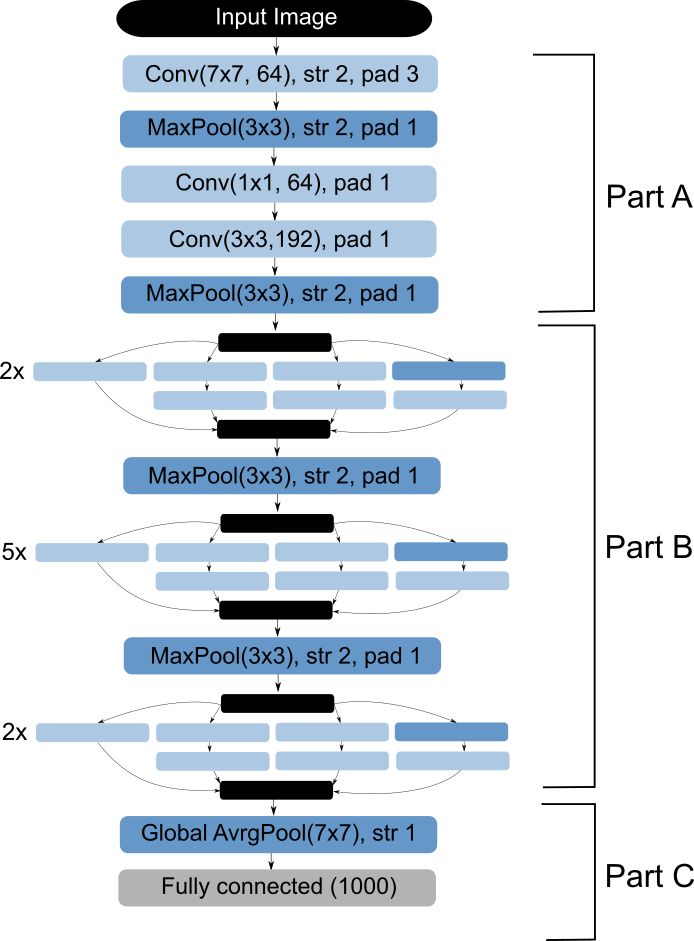
\includegraphics[scale=0.4]{"Part 3 - Learning Systems/Supervised Learning/Deep Learning/images/figure132.png"}
    \caption{ The general structure of the GoogLenet network can be divided into three parts: Part A - Similar to AlexNet and LeNet, contains a sequence of convolutional layers and pooling to reduce image dimensions; Part B - Inceptions modules separated by pooling layers; Part C - Global pooling layer and a Fully Connected for classification \cite{elgendy2020}.}
    \label{fig:googlenet}
\end{figure}

Another technique to make the network more efficient was to include a global AvrgPool layer before the classification layer \cite{geron2019}. In previous CNN models it was common to include flattening to convert the data into a vector, losing the spatial information, to be compatible with the fully connected layers that made the classification. These last layers end up being responsible for most of the parameters. In the VGG-16 model, for example, the 3 fully connected layers generate approximately $123.6$ millions of parameters, almost $90\%$ of the total parameters \cite{johnson2019}.

Instead of adopting flattening, GoogLenet uses an averaging filter of the same dimension as the input element, returning the average of the maps for each position of the vector. As the output vector is already reduced in size, it is necessary to include only one layer fully connected with $1000$ classes. Since the global averaging layer does not need parameters, and since it returns a vector $1024$, approximately $1$ million parameters are needed in the fully connected layer, $100$ times less than in the VGG \cite{johnson2019}. In the last layer, as in the VGG, a Softmax activation is associated, while in the convolution layers it is a ReLu.

The first and last parts of the GoogLenet network have been explained above. The intermediate section that we will study now includes the Inceptions modules that have become characteristic elements of the most modern networks. Each module is similar to VGG blocks, in that some convolutional layers are present in sequence and at the end a pooling layer. In the case of the VGG, it was seen that to reduce the number of hyperparameters, the size of the filters was set to $3\times 3$, and the variable parameter was the number of convolutional layers. The idea of Inceptions (Figure \ref{fig:inceptionmodule}) is not to worry about the size of the filters or the number of layers in the module, as each module consists of a combination of filters with different sizes arranged in a fixed way \cite{elgendy2020}.

\begin{figure}
    \centering
    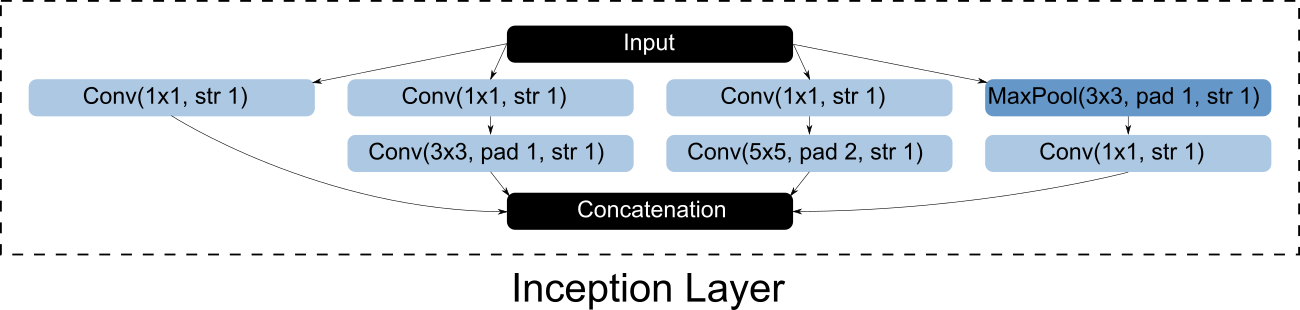
\includegraphics[scale=0.34]{"Part 3 - Learning Systems/Supervised Learning/Deep Learning/images/figure133.png"}
    \caption{ Inception module of the GoogLenet network - The middle part of the GoogLenet network is formed by a sequence of Inceptions modules separated by pooling layers (Figure \ref{fig:googlenet}). Each module has four paths to the same input data, and on output, where the results are concatenated \cite{zhang2020dive}.}
    \label{fig:inceptionmodule}
\end{figure}

From the input of the inception module, copies of the input element go along four paths at the same time. At the end of these paths, the image size does not change, but the number of channels is changed in different ways, with the choice of the number of channels for each layer being a hyperparameter. At the output of the module there is a concatenation of all these channels, forming a single element with the same dimension as at the input and with a number of channels that is the sum of all that resulted from each path.

The first path has only one convolution $1\times 1$, known as the bottleneck, whose main function is to preserve the dimensions (height and width) but reduce the number of channels, which reduces the computational cost and the number of parameters \cite{elgendy2020}. As this convolution includes more nonlinearity at a low cost, a convolution $1\times 1$ is also included in the input layers, contributing to an optimization in the first part of the network \cite{geron2019}. This same layer has been added at the beginning of each of paths 2 and 3 to reduce model complexity. After reducing the number of layers, larger filters are included, making it possible to process information at different scales, with the filters being in the second way $3\times 3$ and in the fourth way  $5\times 5$ \cite{zhang2020dive}.

All paths, even the fourth that includes a MaxPool layer, feature padding to keep the same dimension of the channels as in the entrance. As MaxPool does not change the number of channels, a convolution $1\times 1$ is included at the end of the fourth path, reducing the volume.

By concatenating all the channels of each path at the end, the inception module follows the hypothesis that visual information can be processed at various scales and that the aggregated results allow the next level to extract several features from different scales at the same time \cite{elgendy2020}. In the GoogLenet network in Figure \ref{fig:googlenet}, we see three groups of inception modules interspersed by Maxpooling $3\times 3$, totalling 9 modules.

The previous GoogLenet diagram (Figure \ref{fig:googlenet}) is one of the more simplified representations of the model, because as seen in Figure \ref{fig:googlenet2}, the original architecture includes two classifiers that run in parallel with the other blocks described above, one that starts after the third inception module and the other after the sixth module \cite{geron2019}. Each classifier works similarly to the final part of the network, where classification takes place \cite{johnson2019}. The classifiers are formed by an AvrgPooling layer, followed by a convolution layer, two fully connected layers and at the output a Softmax activation function.

\begin{figure}
    \centering
    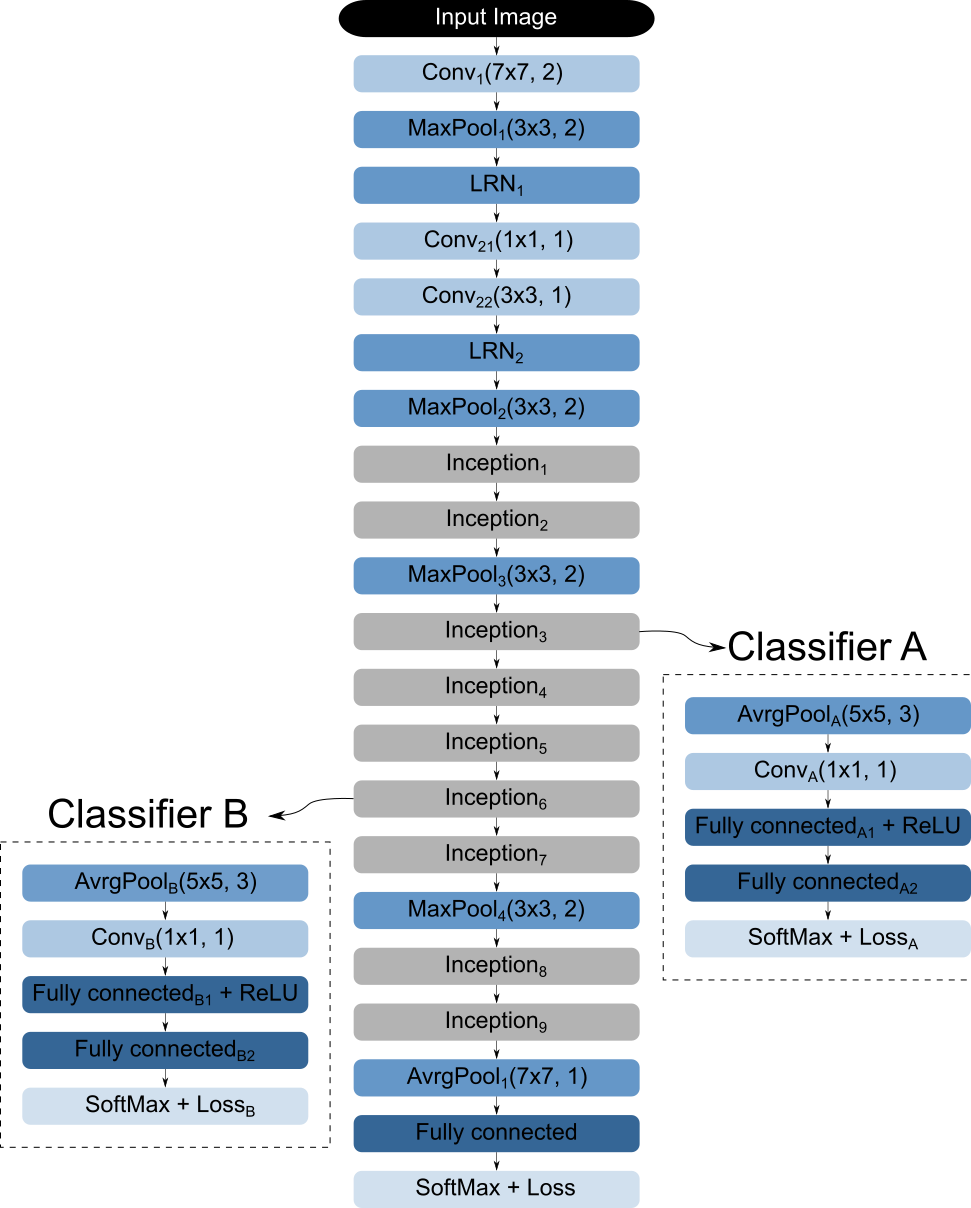
\includegraphics[scale=0.4]{"Part 3 - Learning Systems/Supervised Learning/Deep Learning/images/figure134.png"}
    \caption{GoogLenet network architecture with intermediate classifiers - The GoogLenet network with two classifiers, one in the third inception module and the other in the sixth module. These intermediate classifiers reduce the fading effect of error gradients \cite{img:googlenet}.}
    \label{fig:googlenet2}
\end{figure}


There is a peculiarity when training deeper networks, because, in the backpropagation of errors, the rates reduce to values very close to zero, making it difficult for the algorithm to converge. One of the techniques adopted by GoogLenet to help convergence was to include the calculation of the error gradient of these intermediate classifications in the error backpropagation \cite{geron2019}.


\begin{figure}
    \centering
    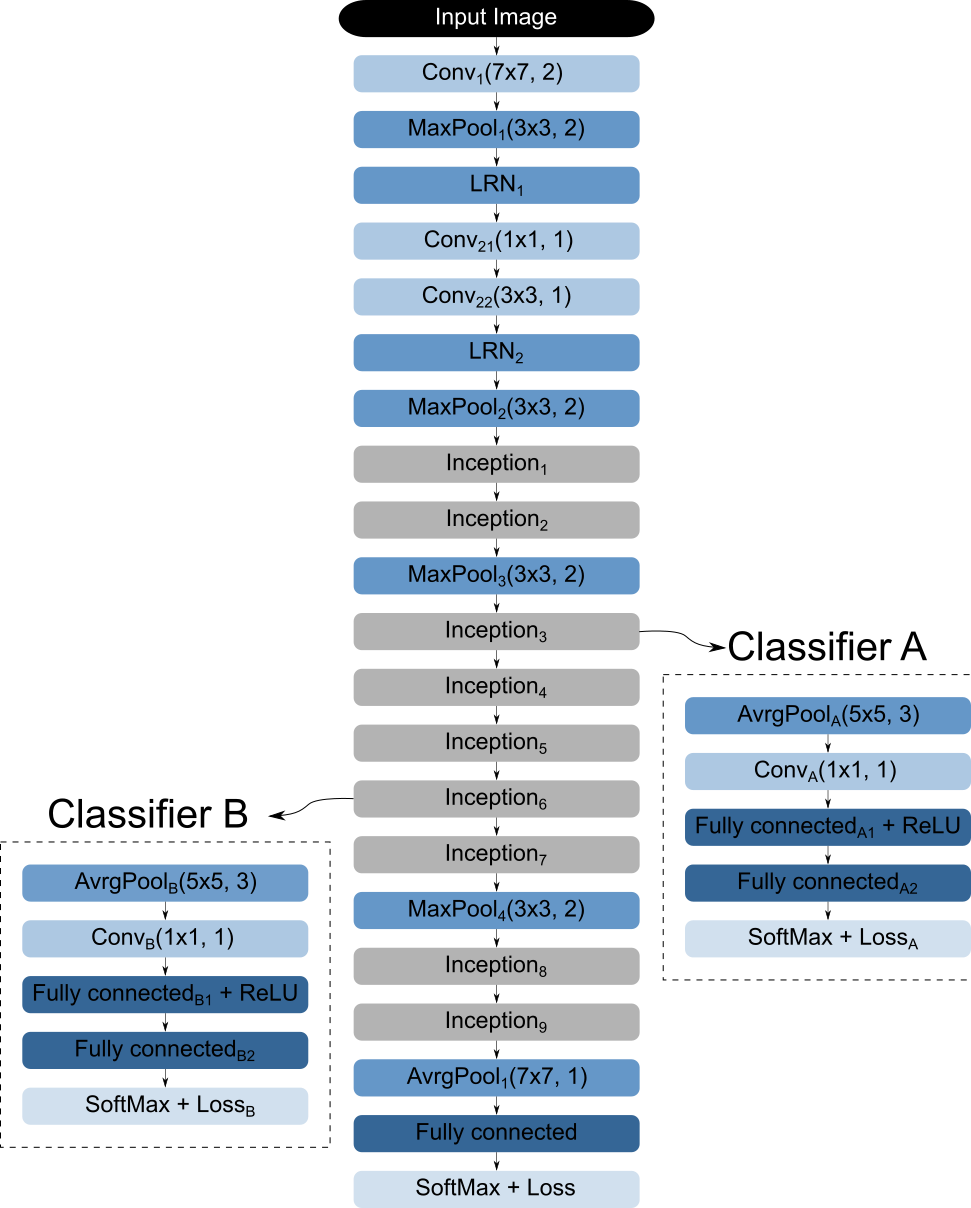
\includegraphics[scale=0.4]{"Part 3 - Learning Systems/Supervised Learning/Deep Learning/images/figure134.png"}
    \caption{GoogLenet network architecture with intermediate classifiers - The GoogLenet network with two classifiers, one in the third inception module and the other in the sixth module. These intermediate classifiers reduce the fading effect of error gradients \cite{img:googlenet}.}
    \label{fig:googlenet2}
\end{figure}

\subsubsection{ResNet}
Residual Neural Network (ResNet) won the ImageNet competition in 2015 with an error rate of 3.6\%. The network developed by a Microsoft research group includes several optimization and regularization techniques from previous models, mainly from GoogLenet. While the characteristic of the GoogLenet network are the inception modules, in ResNet the residual units allowed to train even deeper networks. Among ResNet's main models are nets with 50, 101, 152 layers weights \cite{elgendy2020}, more than double the number of GoogLenet with 22 layers.

Like GoogLenet, the ResNet network can be divided into three parts, the first and last part following the GoogLenet architecture, and the intermediate layers include the residual units. Input layers that allow for a considerable reduction in image size include a convolution layer with 64 channels and 7 x 7 with stride=2 filters, followed by a 3 x 3 MaxPooling layer with stride=2. The last part of the network, the classification structure, has the same layers as GoogLenet, the average Global Pooling layer of dimension 1024 and only a fully connected layer with 1000 units representing the classes. Remembering that the replacement of the flattering process by the global average allowed to reduce the proportion of parameters in the last layers.

\begin{figure}
    \centering
    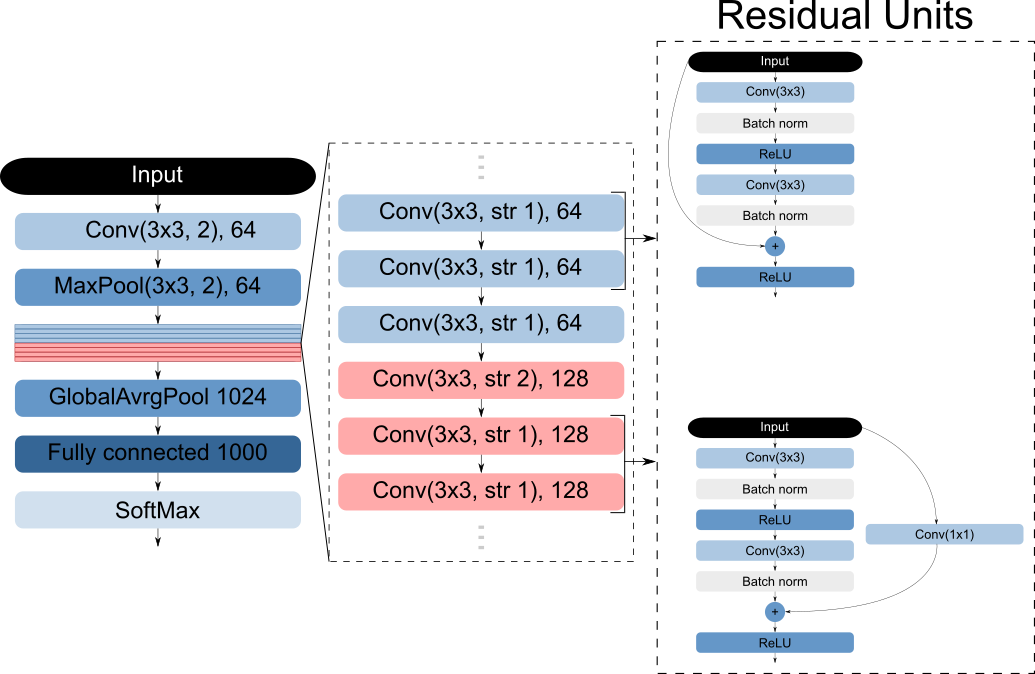
\includegraphics[scale=0.4]{"Part 3 - Learning Systems/Supervised Learning/Deep Learning/images/figure135.png"}
    \caption{ResNet network architecture - The overall structure of the ResNet network can also be divided into three parts. Similar to GoogLenet, it contains a convolutional layer and pooling to reduce image dimensions. A part with residual unit modules, and at the end a global pooling layer and a Full Connect for classification \cite{geron2019}.}
    \label{fig:figure135}
\end{figure}

As described in section GoogleLenet network by adding more layers, the number of parameters can increase in a way that makes training difficult, not only due to the limitations of computational resources, but also due to the possibility of overfitting and delay in the convergence of the algorithm. The GoogLenet model adopted several optimization and regularization approaches, including intermediate classification layers to ensure that the model could converge, avoiding the disappearance of the weights (vanishing gradients), which at times tended to zero \cite{geron2019}.

One of the ResNet techniques that helped to speed up convergence in training was batch normalization. This method became a reference for several CNN models, as until that time each model adopted different approaches to training, such as the intermediate classes of GoogLenet \cite{johnson2019}. Normalization is applied individually by layer, and data normalization occurs based on the statistics of the minibatch clusters adopted in training, which were quickly seen in MLP \cite{zhang2020dive}. In ResNet networks, normalization is applied to the data at the time of transition between the convolution layer and the activation layer.

Even though they managed to converge deeper networks, it was identified in the models that there was a degradation in the accuracy when adding more layers \cite{he2016}. Previously, there was the intuition that when starting from a model with a reduced number of layers to a deeper network, the error should not increase, because at least the deeper network would have part of its layers copied from the other network and the other part would function as identity functions. With more layers, the optimization of a model becomes more complex even for problems easily mapped into smaller networks \cite{he2016}. The idea at ResNet to deal with this complexity was to force the layers to perform the output mapping by including as a reference the input itself, that is, a residual mapping \cite{geron2019}.

In the common mapping of the layers in Figure \ref{fig:figure136}, one imagines that from an training example $\mathbf{x}$, the training seeks to establish an expected response $\mathbf{(x)}$. In the case of residual mapping, a deviation of the input data (x) is included in the output to force a h(x)-x model. This is expected to make it easier to optimize a model with reference, the residual mapping, and that it can quickly adjust to identity functions, ensuring that the layers at least establish the performance of the previous layers \cite{zhang2020dive}. Deviations, residual connections, also minimize the effects of the disappearance of weights, as they allow an alternative flow of gradients, contributing to the back-propagation of the error \cite{elgendy2020}.

\begin{figure}
    \centering
    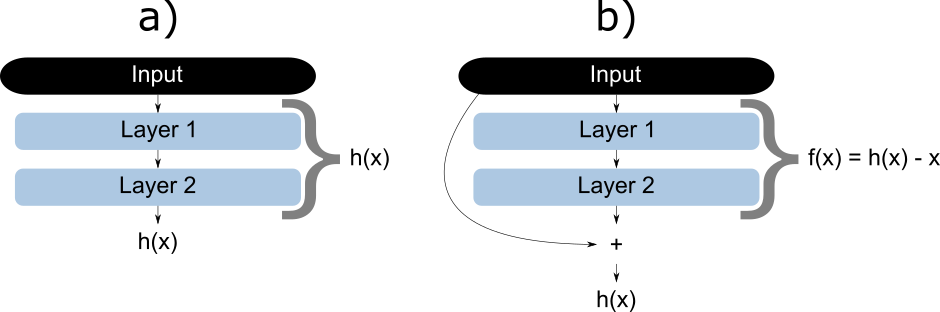
\includegraphics[scale=0.4]{"Part 3 - Learning Systems/Supervised Learning/Deep Learning/images/figure136.png"}
    \caption{Conventional and residual mapping of the ResNet network - a - Traditional mapping of the input and output layers; b - Mapping on a residual unit of the ResNet network. In common mapping, an input x is sought to establish an expected response h(x). The residual model includes an input deviation (x) in the output to force a h(x)-x response \cite{geron2019}}.
    \label{fig:figure136}
\end{figure}

The residual connection starts from the input of a residual unit towards its output, adding the input information with the response before the activation layer ReLu (Figure  \ref{fig:figure137}). Each residual unit has two layers of 3 x 3 convolution, with stride=1 and padding configuration to maintain dimensions. Between the two layers there is a normalization layer preceding a ReLu activation.

\begin{figure}
    \centering
    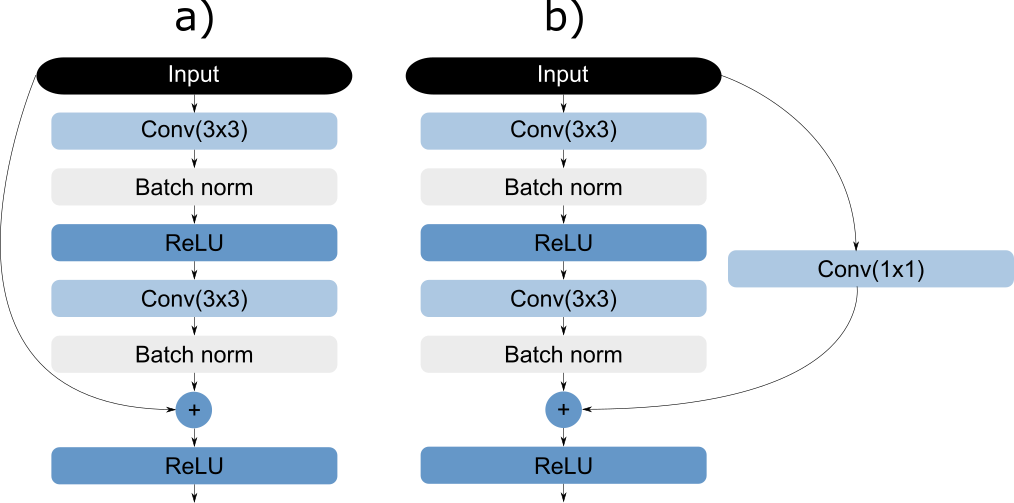
\includegraphics[scale=0.4]{"Part 3 - Learning Systems/Supervised Learning/Deep Learning/images/figure137.png"}
    \caption{Residual unit of the ResNet network - In the middle part of the ResNet network there is a sequence of modules with residual units. Each residual unit has two layers of convolution interspersed by a ReLu activation and a normalization that is also applied to the output of the convolutions \cite{geron2019}}.
    \label{fig:figure137}
\end{figure}

After a sequence of residual units of the same configuration, between the modules, the number of channels is doubled and, at the same time, the width and height of the channels is reduced by half. Between the residual units, no pooling layers are used, thus, to reduce the dimensions of the channels, stride=2 is used in the convolution that encloses a module. In this way, in the last residual unit of the modules, the input has a different dimension than the output. To be able to add the values, it is necessary to correct the dimensions of the input with a 1 x 1 convolution of stride=2 and the same number of channels as the output of the unit    \cite{zhang2020dive}.

The structure of the modules with the residual units resemble the blocks of the VGG network, in which each block presents a sequence of convolution layers with the same dimensions, and always 3 x 3 filter . From one block to another in the VGG, the number of channels also doubles and the height and width are halved, in this case by the MaxPooling effect. ResNet features 4 modules, where the number of residual units varies from model to model as indicated in Figure \ref{fig:figure138}. The ResNet-34, for example, with 34 weight layers contains, respectively, in the four modules, three residual units with 64 channels output, four units with 128 channels, six units with 256 channels and three units with 512 channels \cite{he2016}.

\begin{figure}
    \centering
    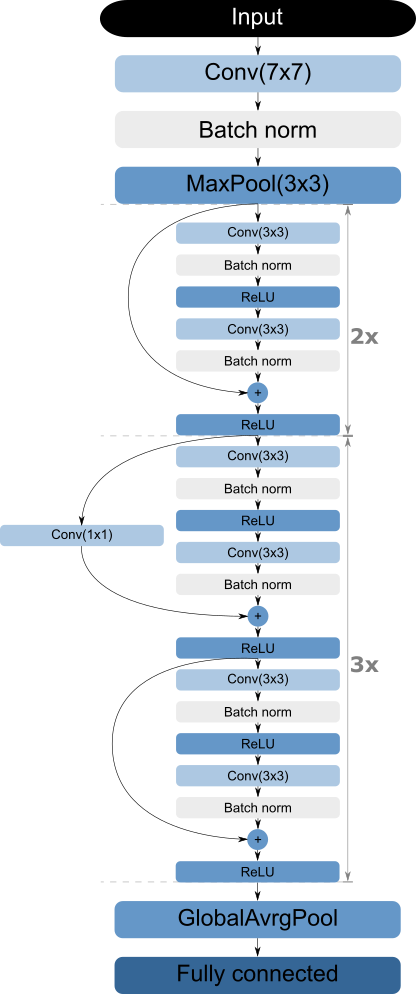
\includegraphics[scale=0.4]{"Part 3 - Learning Systems/Supervised Learning/Deep Learning/images/figure138.png"}
    \caption{ResNet standard architecture - There are several versions of ResNet, with the beginning and the end of the networks being similar, and what usually changes is the amount of residual units in each of the four modules, in the middle part of the network \cite{geron2019}.}
    \label{fig:figure138}
\end{figure}

\section{Transfer learning} \label{transferlearning}
Training a neural network from scratch is a complex task, as it requires an enormous amount of data and computational power \cite{elgendy2020}. In many cases we may not have enough of either, but that doesn't stop us from creating our models. For this we have a technique known as transference learning, which basically consists of using already trained models to solve our problems. In this case we assume that many of the factors that explain the $P_1$ context (situation in which the model was trained) can also explain our new $P_2$ context \cite{goodfellow2016}.

We were able to use this technique because even models trained for different problems end up learning to detect similar characteristics in the earlier layers, with greater specification in the deeper layers. We can see this in Figure \ref{fig:figure139}, where we have the representation of four different networks, the first aimed at working with the image of people, the second with cars, the third with elephants and the last with chairs. Even though these are completely different objects, the networks learn, in the initial layers, to detect edges and corners, which are characteristics shared by all items.

\begin{figure}
    \centering
    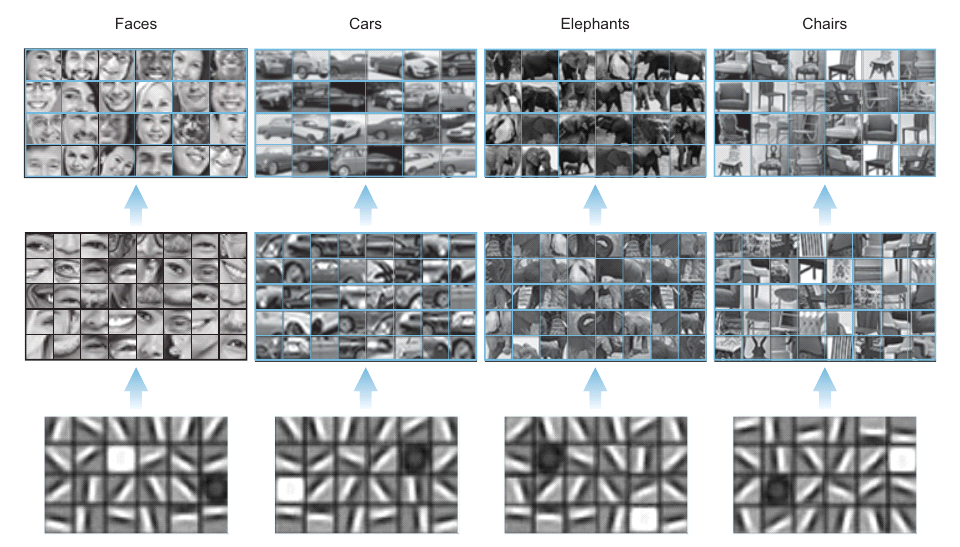
\includegraphics[scale=0.4]{"Part 3 - Learning Systems/Supervised Learning/Deep Learning/images/figure139.png"}
    \caption{Different CNN's and their feature maps in different layers - In the first column we have the features learned by a network specialized in working with human faces, in the second column with cars, in the third with elephants and in the fourth with chairs \cite{elgendy2020}.}
    \label{fig:figure139}
\end{figure}

There are three main ways to carry out the transfer of learning \cite{elgendy2020}, each of which fits better in one scenario or another, they are:

\begin{itemize}
\item Use a pre-trained network as a classifier
\item Use a pre-trained network as a feature extractor
\item Use a pre-trained network for fine tuning
\end{itemize}

The method of using a pre-trained network as a classifier is better when our problem has a domain very similar to the already trained network that we are going to use, as we only have to fit it into our use, not requiring additional training.

The method using a pre-trained network as a feature extractor  is useful when we are solving a problem that has several common features with a pre-trained network but not in a way that we can use as in the previous approach. What we do then is “freeze” the layers of the network that extract features (ie, the layers of convolution) and replace the fully connected network at the end, putting in its place another network that we classify according to our needs, and we train it.

\begin{figure}
    \centering
    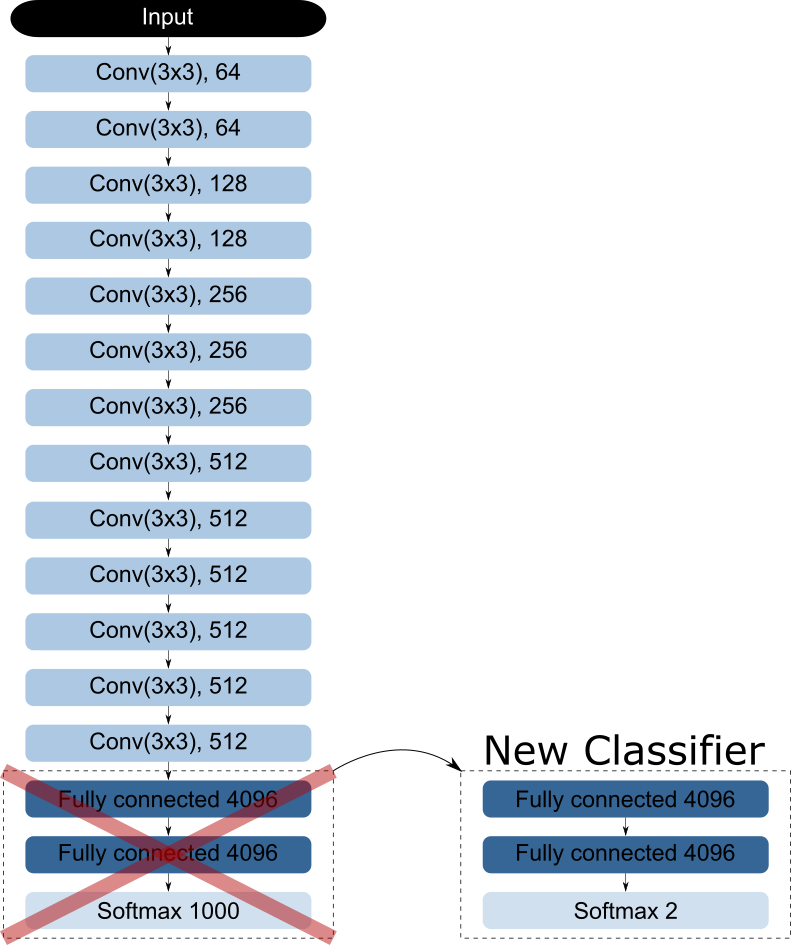
\includegraphics[scale=0.4]{"Part 3 - Learning Systems/Supervised Learning/Deep Learning/images/figure140.png"}
    \caption{VGG-16 Network - We have, from top to bottom, the “frozen” layers, the layers that will be removed and the layer that will be added and trained \cite{elgendy2020}}
    \label{fig:figure140}
\end{figure}

In Figure \ref{fig:figure140}, we have an example from the book by Mohamed Elgendy \cite{elgendy2020}, where he wanted to carry out the classification of dogs and cats. The VGG-16 Network was chosen because it was trained on the ImageNet database, which contains many examples of dogs and cats, so it could adapt well to our problem.

The two previous methods are used when we have a similar domain, since this one, the third method, which uses the pre-trained network for fine tuning, fits into problems that have very different properties. Even in these cases, we were able to use pre-trained networks, for the reasons mentioned above, that networks, especially in their initial layers, learn to detect similar characteristics, becoming more specific according to their depth \cite{elgendy2020}.

In the method that uses the pre-trained network for fine tuning, we have some possibilities. One of them is to “freeze” the first convolutional layers and retrain the rest of the network, what we'll be doing then is fine-tuning (also known as fine-tune) in the deeper layers of the network, so that they can adapt to our current problem. . And the other is not to "freeze" any layer and retrain the entire network, in this case, even having to spend more time and more data is needed, the network tends to converge more quickly to an optimal solution, in comparison to a random initiation \cite{elgendy2020}.

In the book “Deep Learning  for Vision Systems” by Mohamed Elgendy, some tips are presented on how to choose the best learning transfer technique for some types of scenarios, which are presented in Table \ref{table:compareMethods}:

\begin{center}
\begin{table}
    \begin{tabular}{| m{0.14\textwidth} | m{0.14\textwidth} | m{0.30\textwidth} | m{0.25\textwidth} |} \hline
        \textbf{Scenario}& \textbf{Amount of data available}& \textbf{Similarity between the pre-trained network and the new database}& \textbf{Method}\\ \hline
        
        1& Small& Similar& Use a pre-trained network as a classifier\\ \hline
        2& Great& Similar& Fine tune on fully connected network\\ \hline
        3& Small& Very different& Fine-tuning on a part of the network\\ \hline
        4& Great& Very different& Fine tuning across the network\\ \hline
    \end{tabular}
    \caption{Different scenarios where we can use learning transfer (Adapted from \cite{elgendy2020}).}

    \label{table:compareMethods}
\end{table}
\end{center}


\section{Neural networks in practice}
When studying the different models of CNN's we realized that the main factor to improve the accuracy of the networks was the increase in the number of layers, making the networks deeper. It is noteworthy that the construction of deeper models was only possible due to the evolution of hardware performance, especially memory and processing units, and the development of more specific software, known as frameworks for Deep Learning  \cite{zhang2020dive}.

The training of networks involves thousands of operations with multidimensional elements, that is, n-dimensional arrays with arbitrary number of axes, known as tensors \cite{zhang2020dive}. Tensors with only one dimension mathematically correspond to vectors, while tensors with two dimensions are matrices. In the case of CNN's networks, the inputs are often colored images that can be interpreted as three-dimensional tensors: image height, width and volume (RGB channels). Within the network, a series of multiplications and additions takes place from the input tensor, resulting in different three-dimensional tensors.

The performance of all operations is only possible due to the processing units of the machines, which allow the interaction of the arithmetic logic unit (ALU) with the memory. When the first networks were developed, the main processing resource was the CPU's, a general purpose processor where the ALU only performs one calculation at a time. As it has more general applications, it needs constant access to memory for reading instructions and storing data, which is a disadvantage in relation to processing time, known as the “von Neumann bottleneck” (Developers 2021). Generally, to make memory access faster, more sophisticated technologies are integrated into caches, but their size is limited due to cost \cite{zhang2020dive}.

The storage and processing limitations related to a single CPU make it impossible to train deeper networks. What allowed the evolution of networks was the adaptation of processing units with more specific applications. Most modern networks are implemented based on graphics processing units (GPU's). These components were originally developed for graphics applications, mainly for video game rendering \cite{goodfellow2016}. However, much of the GPU's processing approach has also proved to be compatible with the calculations needed to train neural networks.

The GPU achieves greater processing power than a CPU, as it integrates several ALU's in a single processor, which allows thousands of operations to be performed simultaneously (Developers 2021). This strategy is ideal for applications that are suited to parallel processing, such as matrix multiplication in a neural network, which involve independent operations \cite{goodfellow2016}. GPUs were built to perform simpler operations without involving as many branches as is often necessary in CPU workflow. Most network training calculations are predictable, with algorithms that do not require sophisticated controls \cite{goodfellow2016}.

If, on the one hand, network operations do not require great computational complexity, on the other, they demand large amounts of memory. During training you need to store parameters, activation values, and gradients, that is, an amount of data beyond the cache limit associated with the CPU \cite{goodfellow2016}. In this sense, in addition to allowing parallel processing, reducing training time, the GPU also offers a greater amount of memory.

The use of the GPU for training networks became even more common after the adaptation for more general purposes. One of NVIDIA's leading GPU models supports CUDA programming for developing arbitrary code similar to the C language \cite{goodfellow2016}. Thus, the GPU can execute different routines that are not only associated with rendering subroutines.

To ensure high-performance GPU codes, different libraries have been built over the years that deal with numerical computation, mainly involving convolutions and other operations with tensors \cite{goodfellow2016}. Thus, in the development of networks it is not necessary to know the programming at the CUDA level, which is more complex and involves parallel and distributed computing. Generally these libraries, or frameworks, are supported on both GPU and CPU. The first generations of many frameworks were developed through partnerships between Universities and large companies interested in Deep Learning . Some of the more common libraries, highlighted in Table \ref{table:IAframework}, are PyTorch and Caffe2 maintained by Facebook, TensorFlow by Google, MXNet by Amazon, and CNTK by Microsoft \cite{johnson2019}.

\begin{center}
\begin{table}
    \begin{tabular}{| c | c | c |} 
        \hline
        \textbf{Framework}& \textbf{Developer}& \textbf{Predecessor Framework}\\ \hline
        
        Caffe& UC Berkeley& -\\ \hline
        Caffe2& Facebook& Caffe\\ \hline
        Torch& NYU / Facebook& -\\ \hline
        PyTorch& Facebook& Torch\\ \hline
        Theano& U Montreal& -\\ \hline
        TensorFlow& Google& Theano\\ \hline
        PaddlePaddle& Baidu& -\\ \hline
        MXNet& Amazon& -\\ \hline
        Jax& Google& -\\ \hline
        CNTK& Microsoft& -\\ \hline
        Chainer& Community& -\\ \hline

    \end{tabular}
    \caption{Main frameworks for Deep Learning  - To facilitate the manipulation of tensors and the use of GPU's, different frameworks were developed. Most of the first generations of frameworks emerged as partnerships between universities and large companies \cite{johnson2019}.}
    \label{table:IAframework}
\end{table}
\end{center}

Even with the GPU performance increase in relation to the CPU to train the networks, in many cases, a single machine is not enough for all the processing. With the possibility of parallelism, it became common to distribute the workload among several machines. However, building your own GPU network is a high investment, and the technology would also depreciate in a few years as GPU models are rapidly evolving to keep up with growing networks \cite{wangenheim2018}. An alternative for local networks is to use cloud GPU servers offered by providers like Amazon, Google, Microsoft and others.

In recent years, the offer of cloud services to train CNN's has increased, with costs based on the type of GPU technology available, processing time and amount of storage \cite{wangenheim2018}. Some providers offer some free services. The networks can be developed directly on platforms offered by the providers themselves, which generally have an IDE based on Jupyter Notebooks. Each platform has facilities for certain frameworks, usually for those libraries that also provide support \cite{wangenheim2018}. GoogleCloud, for example, features several tools to integrate with TensorFlow.

GoogleCloud offers, in addition to GPU services, the alternative of accessing TPUs as cloud computing resources. The TPU (Tensor Processing Units) is specifically designed to work with neural networks and functions as a specialized matrix processor. As the sequence of calculations is already known, several multipliers and adders were connected, forming a matrix of operators, called systolic matrix (Developers 2021). An advantage of the TPU over CPU and GPU is the reduction of the von Neumann bottleneck, as data is all loaded from memory at once, not requiring access during calculations (Developers 2021).

In the topic about backpropagation an example of an MLP network application for digit recognition that we implemented in the Python language was presented. In the code, the network structure, the training steps and the functions were manually developed, mainly using libraries that deal with calculations in Multidimensional Arrays, such as Numpy. In the MLP example, when manipulating data as numpy's array, no inconsistencies arose and we also didn't face very complex operations, because until that moment the applications didn't involve very dense networks, which required several optimizations and regularizations. In larger network models, using the backpropagation algorithm is a greater challenge and it can often be difficult to ensure convergence just using traditional numerical computation libraries \cite{adrian2017}.

On the other hand, the frameworks we just presented, such as TensorFlow and Pythorch, were built specifically to deal with Deep Learning , and can, for example, automatically provide various optimization and regularization functions. Deep Learning  frameworks generally feature a multidimensional data structure, treated as a tensor class, which replaces the numpy’s “ndarray” \cite{zhang2020dive}. This tensor data structure has some advantages over the traditional numpy array that is better suited to data manipulation in networks. The first point is that numpy defaults to 64 bits precision, whereas tensors generally use 32 bits. Since 32 bitsaccuracy is sufficient to work with networks, reducing data size takes up less memory and makes operations faster \cite{geron2019}.

By default, the manipulation of variables is directed towards calculations in the CPU, however, when different CPU and GPU devices are available, it may be interesting to distribute calculations and storage \cite{zhang2020dive}. Unlike Numpy, Deep Learning  frameworks support handling multiple devices at the same time \cite{zhang2020dive}. Previously we highlighted that the purpose of using GPUs in networks is to speed up training, mainly by adopting distributed and parallel processing, however, if data handling is not adequate, there will be many transfers between devices, thus, processing time may increase \cite{zhang2020dive}. Generally, when using the frameworks configured with the GPU's and CPU's, it is not necessary to worry about how these transfers occur, as the processing is optimized based on computational graphics \cite{geron2019}.

What has made CNN's even more popular even outside academic circles is the development of programming interfaces that make the construction and training of neural networks simpler. Keras, one of the best known APIs for Deep Learning  at a high level, was developed by François Chollet as a research project, which was made available as open source in 2015 \cite{geron2019}. It was written in Python and functions as an underlying computation engine that runs under different backend frameworks, some identified in Figure \ref{fig:figure142}, which support numerical computation, such as TensorFlow, Theano, CNTK, and MxNet \cite{geron2019}.

Much of the work with neural networks can be implemented directly with the high-level API, including the design of the architecture, functions, training algorithm, optimizers and regularization modules. For implementations that need more customization, it is necessary to resort to lower level frameworks, such as TensorFlow, created by a Google research group and released as free software in 2015, has its own keras implementation, tf.keras \cite{geron2019}.

The tf.keras API has only TensorFlow as its backend (Figure \ref{fig:figure142}), but it has greater facilities to integrate with backend customizations. The addition of new codes can be done from the Python language and the API automatically converts to functions of type TensorFlow that are based on C++ \cite{geron2019}. Often these adaptations occur when more control is needed, or to customize functions, layers, regularization modules, initialization processes, or evaluation measures \cite{geron2019}.

Currently the last stable version of TensorFlow is 2.4, the first version of TensorFlow 2.0 being released in March 2019 (Developers 2020). While in versions 1.0, the symbolic module is the central part \cite{geron2019}, mainly due to the preference for the static graphics approach, from versions 2.0 onwards, there was a more imperative programming similar to PyTorch, and that defaults to dynamic graphics \cite{zhang2020dive}. The static module seeks greater code optimization, and after defining the entire process and building the graph, there is no longer any dependence on the code \cite{johnson2019}. In dynamic format, the construction and execution of graphics cannot be unlinked, as they occur simultaneously. Generally, dynamic graphics are easier to debug and have fewer inconsistencies.

\begin{figure}
    \centering
    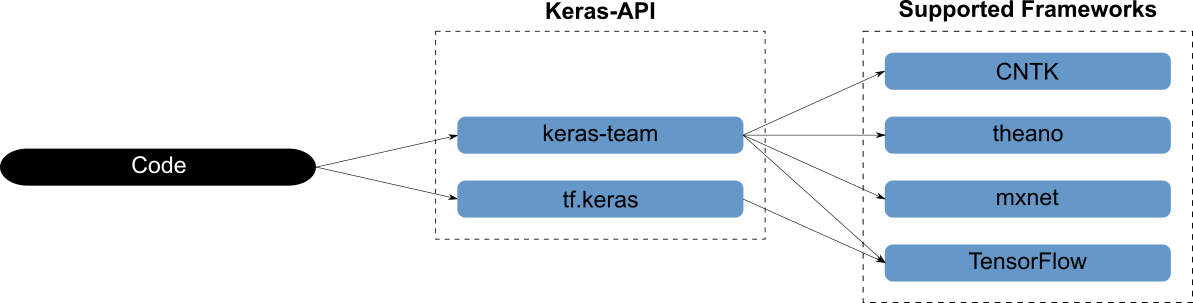
\includegraphics[scale=0.37]{"Part 3 - Learning Systems/Supervised Learning/Deep Learning/images/figure142.png"}
    \caption{ResNet standard architecture - There are several versions of ResNet, with the beginning and the end of the networks being similar, and what usually changes is the amount of residual units in each of the four modules, in the middle part of the network \cite{geron2019}.}
    \label{fig:figure142}
\end{figure}








\newpage
\section{Exercises}
\newcounter{qcounter}
%\begin{list}{
%\textbf{Question \arabic{qcounter}:}~}{\usecounter{qcounter}}

\begin{enumerate}

\iffalse
\item \noindent The perceptron model was one of the first neural network algorithms. One of the limitations that made its application difficult was the restriction of not operating on non-linearly separable problems. This limitation was mainly known when used to simulate logical gates. Computationally assemble the perceptron model to simulate the three types of logic gates (AND, OR, XOR) and comment on the results considering the limitations of the perceptron.


\item \noindent  Based on the MLP network architecture in the figure, construct the MLP network computationally.
\begin{figure}
    \centering
    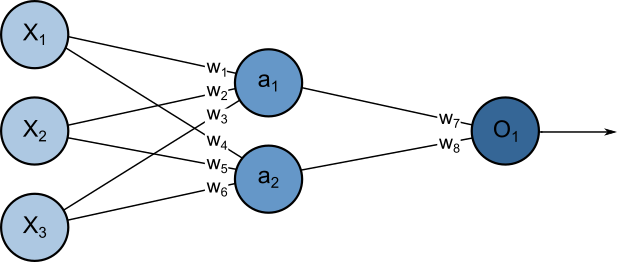
\includegraphics[scale=0.65]{images/backpropagation_ex.png}
    \caption{Simple neural network}
    \label{fig:exercise7}
\end{figure}

\item \noindent The Figure \ref{fig:exercise7} shows a simplified neural network architecture. Do the first backpropagation pass, whereas in the first forward pass, the following operations were made:

$$X \texttt{=}
\left[\begin{smallmatrix}
4 & 3 & 5
\end{smallmatrix}\right]
, 
\text{Desired output}
\texttt{=}
\left[\begin{smallmatrix}
1
\end{smallmatrix}\right]
, 
\left[\begin{smallmatrix}
\text{w}_1 & \text{w}_4\\
\text{w}_2 & \text{w}_5 \\
\text{w}_3 & \text{w}_6
\end{smallmatrix}\right]
\texttt{=}
\left[\begin{smallmatrix}
0.12 & 0.33\\
0.5 & 0.7 \\
0.15 & 0.45
\end{smallmatrix}\right]
\text{and}
\left[\begin{smallmatrix}
\text{w}_7 \\
\text{w}_8
\end{smallmatrix}\right]
\texttt{=}
\left[\begin{smallmatrix}
0.13 \\
0.6
\end{smallmatrix}\right]
$$

$$\left[\begin{smallmatrix}
4 & 3 & 5
\end{smallmatrix}\right]
\cdot 
\left[\begin{smallmatrix}
0.12 & 0.33\\
0.5 & 0.7 \\
0.15 & 0.45
\end{smallmatrix}\right]
=
\left[\begin{smallmatrix}
2.73 & 5.67 
\end{smallmatrix}\right]
\rightarrow
\text{sigmoid}(\left[\begin{smallmatrix}
2.73 & 5.67 
\end{smallmatrix}\right])
=
\text{a}
=
\left[\begin{smallmatrix}
0.94 & 0.99 
\end{smallmatrix}\right]
$$

$$\left[\begin{smallmatrix}
0.94 & 0.99 
\end{smallmatrix}\right]
\cdot 
\left[\begin{smallmatrix}
0.13\\
0.6 
\end{smallmatrix}\right]
=
\left[\begin{smallmatrix}
0.71
\end{smallmatrix}\right]
\rightarrow
\text{sigmoid}(\left[\begin{smallmatrix}
0.71
\end{smallmatrix}\right])
=
\text{O}_1
= 
\left[\begin{smallmatrix}
0.67
\end{smallmatrix}\right]
$$

$$
\text{Error}
=
\frac{1}{2}(0.67-1.0)^2=0.05445
$$


\item The MNIST dataset contains images of numbers from 0 to 9, with each of these images being $28$x$28$ in size. Implement a neural network to sort the digits, considering that the input will have a dimension of $28$x$28=784$, use $30$ nodes in the hidden layer and finally $10$ positions in the output. Once implemented, perform tests varying the number of epochs and the amount of data to evaluate the accuracy behavior using graphics.


\item There are different error functions that can be used during the training of a neural network, as an example we have the cross entropy, the mean square error, among others. Considering the network implemented in the previous exercise, choose another error function to change the algorithm and then compare the results of the two models.
\fi

\item \noindent Considering the focus on convolutional neural networks, we can highlight convolution as a basic operator. For a basic understanding of the application and effect of convolution, manually convolute the $\left[\begin{smallmatrix}
0 & 2 & 3\\
0 & 1 & 0\\
3 & 0 & 2
\end{smallmatrix}\right]$ onto the $\left[\begin{smallmatrix}
1 & 2 & 0\\
3 & 0 & 0\\
4 & 1 & 0
\end{smallmatrix}\right]$ and compare with the computationally calculated result. 


\item \noindent The combination of convolutions allows networks to learn at different levels of information about the object of study. In the context of applications with images, each convolution layer can identify a level of detail, for example, in the initial layers there are more general elements of the images, such as lines, edges and corners. Some filters, or convolutions, that have the edge detection property are Sobel and Prewitt. Apply each filter to an image and compare the results.


\begin{itemize}
\item Prewitt Operators. By applying each operator on the image and performing the sum of the modulus of each result, it is possible to determine the edges in the image.

$G_x= \left[\begin{smallmatrix}
-1 & 0 & 1\\
-1 & 0 & 1\\
-1 & 0 & 1
\end{smallmatrix}\right]$

$G_y = \left[\begin{smallmatrix}
-1 & -1 & -1\\
 0 &  0 &  0\\
 1 &  1 &  1
\end{smallmatrix}\right]$

\item Sobel Operators. By applying each operator on the image and performing the sum of the modulus of each result, it is possible to determine the edges in the image.

$G_x= \left[\begin{smallmatrix}
-1 & 0 & 1\\
-2 & 0 & 2\\
-1 & 0 & 1
\end{smallmatrix}\right]$

$G_y = \left[\begin{smallmatrix}
-1 & -2 & -1\\
 0 &  0 &  0\\
 1 &  2 &  1
\end{smallmatrix}\right]$

\end{itemize}

\item \noindent One of the techniques used in image applications using convolutional neural networks is to reduce the size of inputs across layers, which can reduce computational costs. To perform this reduction we can use strides in the application of convolution. Perform the convolution between kernel $\left[\begin{smallmatrix}
0 & 2 & 3 \\
0 & 1 & 0 \\
3 & 0 & 2 
\end{smallmatrix}\right]$ and matrix  $\left[\begin{smallmatrix}
1 & 2 & 0 & 3 & 0\\
3 & 0 & 0 & 1 & 0\\
4 & 1 & 0 & 2 & 1
\end{smallmatrix}\right]$, first using stride 1 and then with stride 2 to assess the effect of this technique. 


\item \noindent During image processing in convolutional neural networks, there are steps in which the inputs and outputs of the convolution layers need to keep the same size, and one way to have this control is to use padding in the application of the convolution. With the same kernel and matrix as in the previous exercise, determine a padding to ensure that the result remains the same size as the original matrix, and then apply the convolution using this padding.


\item \noindent The LeNeT network is one of the simplest convolutional networks, being possible to implement without the use of frameworks and still obtain good results in a short period of testing time. Using the MNIST dataset build a LeNet network for digit classification, with and without framework. Evaluate the implementation complexity in the two cases and the results considering the same input and training parameters.


\item The construction of a Convolutional Neural Network for classification of cats and dogs images is a very common exercise, usually performed to demonstrate the most important ideas in the functioning of CNNs. That said, use some dataset that contains images of dogs and cats (like the one available in the TensorFlow library\footnote{\url{https://www.tensorflow.org/datasets/catalog/cats_vs_dogs}}) and use it to compare the performance of the AlexNet, VGG and GoogleLeNet networks (remembering that these models are already available, fully pre-trained, in libraries such as Keras\footnote{\url{https://keras.io/api/applications/}} and Pytorch\footnote{\url{https://pytorch.org/vision/stable/models.html}}).


\item As explained in the Transfer Learning section \ref{transferlearning}, Convolutional Neural Networks with large and complex architectures can take a long time and consume large amounts of processing and memory in their training. Using pre-trained networks can help us, as we can use them directly or train them from that point on. Like in the previous exercise, use pre-trained models from some library, but this time using a dataset with a larger number of classes (for example, the cifar100 dataset\footnote{\url{https://www.tensorflow.org/datasets/catalog/cifar100}} that contains 100 classes). Also check the difference in performance of each model, taking into account its complexity and the number of classes.
%\end{list}
\end{enumerate}

\bibliographystyle{unsrt}
\bibliography{bibliography}

\end{document}
